% STEP 1: Choose oneside or twoside. Use the 'draft' option a lot when writing.
\documentclass[english, oneside]{HYgradu}

\usepackage[utf8]{inputenc} % For UTF8 support. Use UTF8 when saving your file.
\usepackage{lmodern} % Font package
\usepackage{textcomp}
\usepackage[pdftex]{color, graphicx} % For pdf output and jpg/png graphics
\usepackage[pdftex, plainpages=false]{hyperref} % For hyperlinks and pdf metadata
\usepackage{fancyhdr} % For nicer page headers
%\usepackage{tikz} % For making vector graphics (hard to learn but powerful)
%\usepackage{wrapfig} % For nice text-wrapping figures (use at own discretion)
\usepackage{amsmath, amssymb} % For better math
\usepackage[round]{natbib} % For bibliography
\usepackage[footnotesize,bf]{caption} % For more control over figure captions
\usepackage{subcaption}
\usepackage{arydshln}

\fussy % Probably not needed but you never know...


% OPTIONAL STEP: Set up properties and metadata for the pdf file that pdfLaTeX makes.
% But you don't really need to do this unless you want to.
\hypersetup{
    bookmarks=true,         % show bookmarks bar first?
    unicode=true,           % to show non-Latin characters in Acrobat’s bookmarks
    pdftoolbar=true,        % show Acrobat’s toolbar?
    pdfmenubar=true,        % show Acrobat’s menu?
    pdffitwindow=false,     % window fit to page when opened
    pdfstartview={FitH},    % fits the width of the page to the window
    pdftitle={},            % title
    pdfauthor={},           % author
    pdfsubject={},          % subject of the document
    pdfcreator={},          % creator of the document
    pdfproducer={pdfLaTeX}, % producer of the document
    pdfkeywords={something} {something else}, % list of keywords for
    pdfnewwindow=true,      % links in new window
    colorlinks=true,        % false: boxed links; true: colored links
    linkcolor=black,        % color of internal links
    citecolor=black,        % color of links to bibliography
    filecolor=magenta,      % color of file links
    urlcolor=cyan           % color of external links
}

% STEP 2:
% Set up all the information for the title page and the abstract form.
% Replace parameters with your information.
\title{Formation of cores by merging supermassive black holes}
\author{Joonas Suortti}
\date{\today}
\level{Master's thesis}
\faculty{Faculty of Whatever}
\department{Department of Something}
\address{PL 42 (Kuvitteellinen katu 1)\\00014 Helsingin yliopisto}
\subject{Your Field}
\prof{prof. Smith}
\censors{prof. Smith}{doc. Smythe}{}
\depositeplace{}
\additionalinformation{}
\numberofpagesinformation{\numberofpages\ pages}
\classification{}
\keywords{Your keywords here}
\quoting{``Bachelor's degrees make pretty good placemats if you get them laminated.'' \\---Jeph Jacques}

\begin{document}

% Generate title page.
\maketitle

%\onehalfspacing
\doublespacing

% STEP 3:
% Write your abstract (of course you really do this last).
% You can make several abstract pages (if you want it in different languages),
% but you should also then redefine some of the above parameters in the proper
% language as well, in between the abstract definitions.
\begin{abstract}
Abstract goes here.
\end{abstract}

% Place ToC
\mytableofcontents



% -----------------------------------------------------------------------------------
% STEP 4: Write the thesis.
% Your actual text starts here. You shouldn't mess with the code above the line except
% to change the parameters. Removing the abstract and ToC commands will mess up stuff.
\chapter{Introduction}

\chapter{Background Theory}

\section{Elliptical Galaxies} \label{section:elliptical}

\subsection{Basic Properties and Classification}

Elliptical galaxies (Es) are galaxies characterised by their ellipsoidal shape, lack of a rapidly rotating disk, tendency to be very massive, and their small or essentially almost non-existent content of cool gas and dust. Furthermore, due to the absence of star formation caused by the lack of dust and cool gas, the stellar population of elliptical galaxies is generally quite old, with a mean age of $\gtrsim{10} \; \mathrm{Gyr}$ \citep{GalaxyFormationAndEvo2010}. This correlates well with their observed red colours \citep{Cappellari2016}, as stellar spectra tend to become redder with age.

Elliptical galaxies are included in the Hubble classification of galaxies \citep{Hubble1926}. In the Hubble "tuning-fork diagram" (figure \ref{figure:tuning_fork}), they are located left of the point where the sequence diverges into the two spiral galaxy paths. This means that alongside lenticular galaxies, which are transitional objects between elliptical and spiral galaxies, elliptical galaxies are so-called "early-type galaxies" (ETGs). ETGs are, in fact, often defined simply as galaxies that do not contain spiral arms.

\begin{figure}
	\centering
	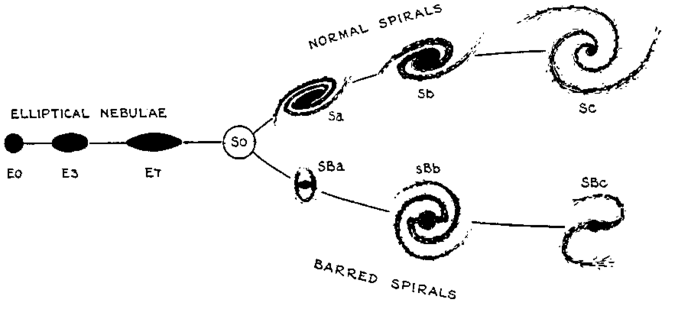
\includegraphics[width=\textwidth]{TuningForkHubble.png}
	\caption{The Hubble tuning-fork diagram. The image is originally is from \cite{Hubble1936}.}
	\label{figure:tuning_fork}
\end{figure}

In the Hubble classification, elliptical galaxies are further divided into seven different subcategories according to their observed apparent ellipticity. These categories range from E0 to E7, where the number denotes the ellipticity of the galaxy multiplied by ten and rounded to the nearest integer. The ellipticity of a galaxy is simply the measure of how flattened an observed 2D-projection of a ellipsoidal stellar system is. It can be calculated using the equation:
\begin{equation}
\epsilon = 1 - \frac{b}{a},
\end{equation}
where $a$ and $b$ are the semi-major and semi-minor axes of a luminosity isophote (i.e. constant luminosity or surface brightness contour), respectively. The larger the ellipticity, the flatter the system ($\epsilon = 0$ denotes a completely spherical galaxy). It is important to note, however, that the ellipticity of a system can depend on the specific isophote from which it is calculated. Since the isophotes of elliptical galaxies generally become flatter the farther they are located from the galactic centre \citep{BinneyTremaine}, this could result in a single galaxy having multiple ellipticities. To remedy this, the Hubble classification uses the ellipticity at the effective radius ($R_e$) to determine the subcategory of an elliptical galaxy. The effective radius is the radius of a sphere that encloses half of the total luminosity of the galaxy. Since galaxies do not have clearly defined boundaries, $R_e$ is also often used as their measure of size. 

\subsection{Photometry} \label{section:ellip_photo}

The photometric properties of elliptical galaxies are often described in terms of the surface brightness, which describes the amount of observed luminosity from a unit area. Thus, an important property for studying the general spatial distribution of stellar material in the observed elliptical galaxies, is the one-dimensional radial surface brightness profile $I(R)$, where $R$ is the projected distance from the centre of the galaxy. In practice, these profiles can be constructed by calculating the azimuthal averages of observed surface brightness at every projected radius $R$ \citep{MerrittBook}.

The observed surface brightness profiles of elliptical galaxies are typically smooth and featureless, declining smoothly as the projected radius grows, until the galaxy is indistinguishable from the background \citep{BinneyTremaine}. The observed "power-law"-like profiles are quite similar in shape across all elliptical galaxies, which has led to the formulation of a multitude of models that attempt to describe this general shape. An early example of such a model is the "de Vaucouleurs" power-law profile: $I \propto R^{1/4}$ \citep{deVaucouleurs1948}. This profile, however, is quite simple, and only represents well the profiles of some elliptical galaxies, namely the bright ellipticals \citep{MerrittBook}. 

Compared to the de Vaucoulers-profile, a more robust and more commonly used model is the Sérsic-profile \citep{Sersic1968}:
\begin{equation}
I (R) = I_e \exp \{ -b_n \left[ (R / R_e)^{1/n} \right] \},
\end{equation}
where $R$ is the projected distance from the galactic centre, $I_e$ is the surface brightness at the effective radius, $n$ is the so-called Sérsic index ($n=4$ gives a Sérsic profile which is identical to the de Vaucouleurs profile), and $b_n$ is a shape factor, which is defined so that a circular area with a radius of $R_e$ contains half of the total luminosity of the galaxy. The value for the shape factor can be approximated as $b_n \approx 2n - 0.324$, when $1 \lesssim n \lesssim 10$ \citep{BinneyTremaine}. 

The prominent use of the Sérsic-profile is due to the fact, that it describes the observed surface brightness profiles of many different elliptical galaxies very well for a large range of radii \citep{MerrittBook}. However, when extrapolated to the central regions of galaxies, the profile often deviates from the observations. \cite{Kormendy2009} find that there are two kinds of deviations. The galactic cores either contain "missing" or "extra" light, corresponding to, what are often called, "cored" or "cuspy" central surface brightness profiles, respectively.

Whether the central surface brightness profile of an elliptical galaxy is a shallow "cored" profile or a steep "cuspy" profile is seemingly tied to the absolute magnitude of the galaxy. Typically, bright ellipticals ($\mathcal{M_V} \lesssim -22$) have central profiles with missing light, while fainter galaxies ($-22 \lesssim \mathcal{M_V} \lesssim -16$) contain extra light at their centres \citep{Kormendy2009}. 

This supposed dichotomy between the brighter and fainter ellipticals also extends to the isophotal shapes of the galaxies. Usually the shapes of the isophotes of elliptical galaxies deviate from exact ellipses, and the brighter ellipticals contain so-called "boxy" isophotes, while the isophotes of the fainter galaxies are typically more "disky" (an illustration of the two isophotal shapes can be seen in figure \ref{figure:isophotes}) \citep{GalaxyFormationAndEvo2010}. Whether the shapes of the isophotes are "boxy" or "disky", can be determined from the Fourier-series of the deviations of the observed isophotes from their respective best-fit ellipses, which is described by the following formula:
\begin{equation}
\Delta (\phi) = R_\mathrm{iso}(\phi) - R_\mathrm{ell}(\phi) = a_0 + \displaystyle\sum^\infty_{n=1} (a_n \cos(n\phi) + b_n \sin(n\phi)), \label{eq:isophote_deviations}
\end{equation}
where $R_\mathrm{iso}(\phi)$ is the radius of the isophote at the angle $\phi$, $R_\mathrm{ell}(\phi)$ is the radius of the corresponding perfect ellipse at the same angle, and where $a_n$ and $b_n$ are the Fourier coefficients. If $a_4 < 0$ holds true the isophote is "boxy", and if $a_4 > 0$ holds true the shape of the isophote is deemed "disky".

\begin{figure}
	\centering
	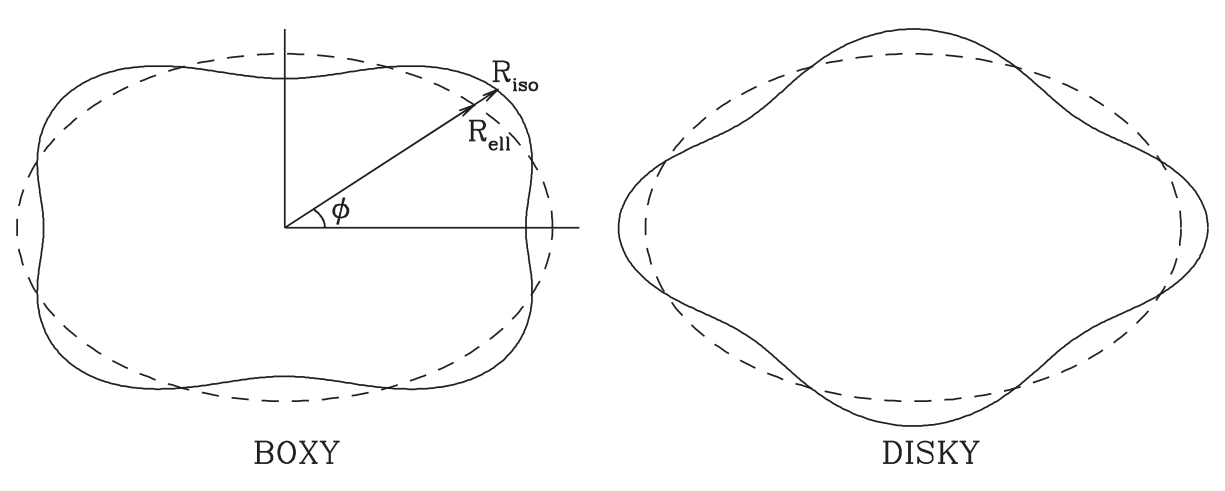
\includegraphics[width=\textwidth]{boxy_and_disky_GFE.png}
	\caption{A comparison between the isophotal shapes of "boxy" and "disky" galaxies. The solid curves denote the respective isophotal shape, while the dashed lines denote their best-fit ellipses. The markings on top of the picture of the "boxy" isophote illustrate the procedure described by equation \ref{eq:isophote_deviations}. This picture is originally from \cite{GalaxyFormationAndEvo2010}.}
	\label{figure:isophotes}
\end{figure}

\subsection{Kinematics} \label{section:ellip_kinematics}

The divide between bright and faint elliptical galaxies, specified in the previous section, seems to also include the kinematics of the galaxies \citep[discussed in e.g.][]{GalaxyFormationAndEvo2010}. The brighter galaxies rotate slowly ($V/\sigma \lesssim 0.1$; where $V$ and $\sigma$ are the line-of-sight maximum velocity and the velocity dispersion at the centre of the galaxy, respectively), while the rotation of the faint galaxies is faster ($V/\sigma \sim 1$) \citep{Davies1983, Cappellari2007}. Furthermore, the velocity distributions of the bright "boxy" galaxies are relatively anisotropic, with a large amount of random stellar motion compared to the amount of ordered motion (i.e. small $V/\sigma$ values); which contrasts with the more isotropic and ordered velocity distributions (thus larger $V/\sigma$ values) of the fainter and more disk-like galaxies \citep{Kormendy2009, Krajnovic2008}. 

\begin{figure}[h]
	\centering
	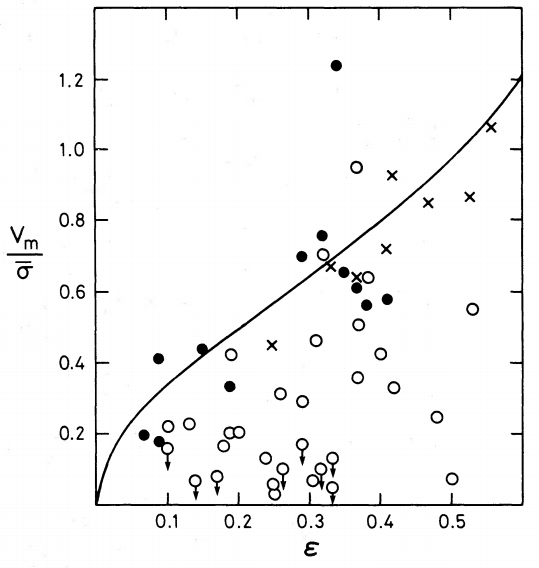
\includegraphics[width=0.60\textwidth]{davies_v-sigma.png}
	\caption{Plot of the relation between $V/\sigma$ and $\epsilon$ in observed galaxies. The solid curve is defined by equation \ref{eq:v-sigma-epsilon} and shows the expected relation for galaxies with isotropic rotation. The filled circles denote elliptical galaxies with a $B$-band magnitude of $M_B > -20.5$, while the open circles are for galaxies with $M_B < -20.5$. The crosses stand for bulges of disk galaxies. The figure is originally from \cite{Davies1983}.}
	\label{figure:v-sigma}
\end{figure}

The more ordered and faster rotation of the fainter galaxies seems to be, at least in part, consistent with rotational flattening. For isotropic rotators, the value of $V/\sigma$ parameter is expected to approximately follow the equation:
\begin{equation}
\frac{V}{\overline{\sigma}} \approx \sqrt{\frac{\epsilon}{1-\epsilon}}, \label{eq:v-sigma-epsilon}
\end{equation}
where $\overline{\sigma}$ is the mean velocity dispersion inside half of the effective radius and $\epsilon$ is the ellipticity of the galaxy. This gives a relation between the rotation and the expected ellipticity noted as the $V/\sigma$ – $\epsilon$-relation. Figure \ref{figure:v-sigma} shows the expected $V/\sigma$ – $\epsilon$ relation described by equation \ref{eq:v-sigma-epsilon} as a curve, alongside the observed apparent ellipticities and $V/\sigma$ parameters for elliptical galaxies with a $B$-band magnitude of either $M_B > -20.5$ (filled circles) or $M_B < -20.5$ (open circles) \citep{Davies1983}. By looking at the figure, it is clear that, when compared to the brighter galaxies, the fainter galaxies are, in general, situated closer to the curve describing the expected relation. This implies that, unlike the boxy bright ellipticals, the fainter disky ellipticals are flattened by rotation. The flattening of the brighter galaxies is then usually attributed to stresses caused by their anisotropic velocity distributions \citep{Davies1983}.

A further distinction between the bright and relatively faint ellipticals can be drawn from their gravitational potentials. While the "disky" galaxies are assumed to be axisymmetric, with an ellipsoidal shape containing two identical-length semi-principal axes ($A = B \neq C$); the "boxy" galaxies seem to be triaxial, with all of their semi-principal axes having different lengths ($A \neq B \neq C$) \citep{GalaxyFormationAndEvo2010}. 

The triaxial potential of the bright ellipticals can be identified from the fact, that unlike the fainter galaxies, bright Es often contain kinematic misalignments, meaning that the position angle of their projected kinematic axis differs from their photometric minor axis. According to \cite{GalaxyFormationAndEvo2010}, these misalignments can arise as a result of two different effects. A kinematic misalignment might be caused by, a misalignment between the projected and the apparent observed minor axes of the galaxy, which is common for triaxial galaxies due to their asymmetric shape. On the other hand, the deviation in the position angles might also be the result of the observed galaxy having intrinsically misaligned angular momentum, which would be a natural consequence of triaxial potentials supporting rotation around all three axes. Both of these effects require the host galaxy to be triaxial.

\begin{figure}
	\centering
	\begin{subfigure}[b]{0.49\textwidth}
		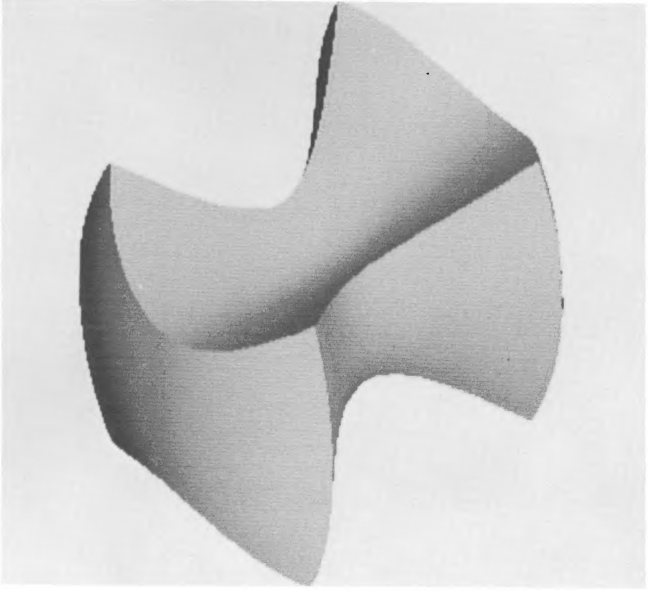
\includegraphics[width=\textwidth]{statler_box.png}
		\caption{Box-orbit}
	\end{subfigure}
	\begin{subfigure}[b]{0.49\textwidth}
		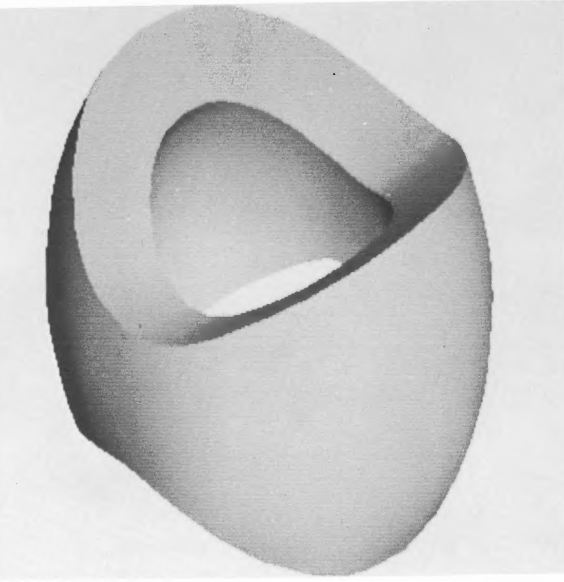
\includegraphics[width=\textwidth]{statler_short_tube.png}
		\caption{Short-axis tube-orbit}
	\end{subfigure}
	\begin{subfigure}[b]{0.49\textwidth}
		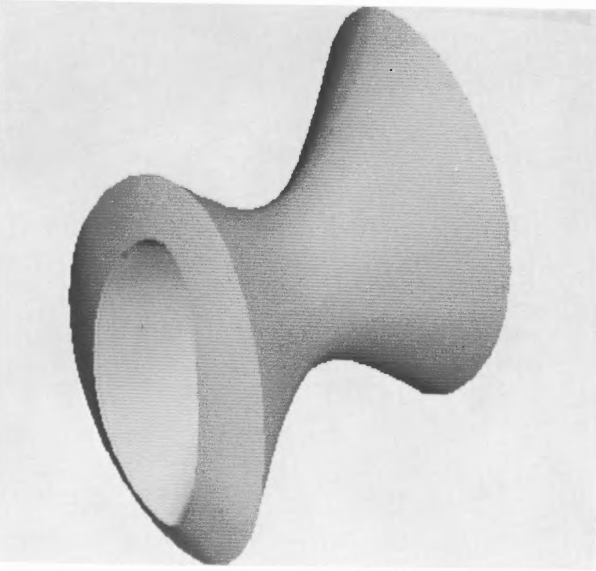
\includegraphics[width=\textwidth]{statler_long_inner.png}
		\caption{Inner long-axis tube-orbit}
	\end{subfigure}
	\begin{subfigure}[b]{0.49\textwidth}
		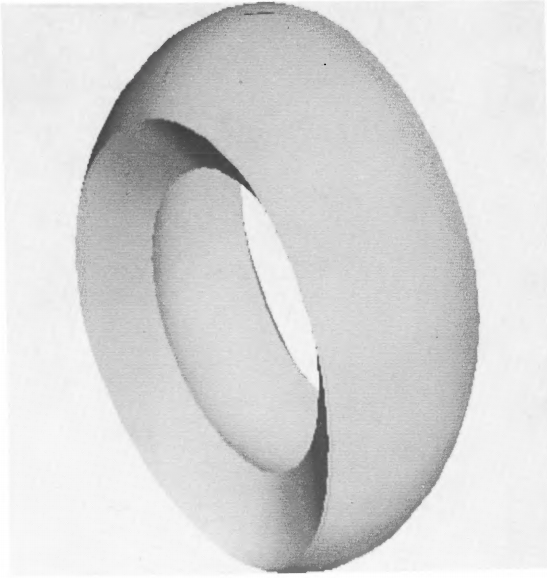
\includegraphics[width=\textwidth]{statler_long_outer.png}
		\caption{Outer long-axis tube-orbit}
	\end{subfigure}
	\caption{Models of the different types of orbits in triaxial potential. The figures are from \cite{Statler1987}.}
	\label{figure:triaxial_orbits}
\end{figure}

Depending on the shape of its gravitational potential, galaxies support different kinds of orbits. Axisymmetric potentials support both so-called tube-orbits, which are orbits that trace a ring-like volume around the axis-of-symmetry; and the cone-shaped saucer-orbits \citep{MerrittBook}. Triaxial galaxies support four different types of orbits, models of which can be seen in figure \ref{figure:triaxial_orbits}. Similarly to axisymmetric potentials these include tube orbits, though in the case of a triaxial potential, they can trace a volume around either the short axis, inner long axis or outer long axis. The fourth orbital type is the box-orbit, which is an orbit that fills a rectangular volume. Stars on box-orbits can move through the centre of the galaxy, and are often the dominant stellar component in triaxial potential models, giving the "boxy" galaxies their characteristic shape \citep{BinneyTremaine}.

%Slowly rotating bright ellipticals often exhibit so-called \textit{Kinematically Distinct Cores} (KDCs). KDCs are central regions of galaxies with an angular momentum that has a different or even opposite direction when compared to the rest of the galaxy. Once again, the existence of a KDC in a galaxy might point to the host being triaxial, as they could simply be projections of major families of circulating orbits in a triaxial potential \citep{Statler1991, GalaxyFormationAndEvo2010}.% It is also possible, however, that the KDCs have formed from the accretion of other galaxies onto the host galaxy, meaning that they might not be able to be used as markers of triaxial potentials.

\subsection{Formation Models}

There are two main models for the formation of elliptical galaxies: the monolithic collapse scenario and the merger scenario \citep{GalaxyFormationAndEvo2010}. In the monolithic collapse scenario, elliptical galaxies are formed through the collapse and stabilization of some initial condition, which results in the simultaneous formation of the stellar material and the assembly of the galaxy. This collapse can either be "dissipative" or "dissipationless". In a dissipative process, the system loses some of its total energy through radiation; which, in the case of galaxy formation through monolithic collapse, often means that the initial condition contains some gaseous component, which turns into stars as it collapses. On the other hand, if a process is dissipationless, the total energy is conserved. For the formation of galaxies, this usually necessitates a lack of gaseous components in the initial conditions. 

Assuming that the collapse in the monolithic collapse scenario is dissipative, the model in question is able to reproduce several features observed in actual ellipticals, such as the observed lack of dark matter in the central regions of galaxies \citep{GalaxyFormationAndEvo2010}. However, main problem of the monolithic collapse scenario is that it is not compatible with the current paradigm that expects a $\Lambda CDM$ cosmology for the universe. 

The cold dark matter (CDM) cosmology assumes a hierarchical formation for the observed structures, where star formation and the merging of dark matter halos are still on-going processes. This is in stark contrast to the monolithic collapse scenario, where after the initial collapse, the resulting stellar system evolves mostly passively, without experiencing either major galaxy mergers or star-formation.

The merger scenario, on the other hand, suggests that elliptical galaxies are formed through mergers of two or more pre-existing fully formed galaxies \citep{GalaxyFormationAndEvo2010}. Thus, the formation of stars and the assembly of the final galaxy are independent of each other. Since the star formation and the assembly of the galaxy are once again largely independent from each other, even this formation scenario can not be reconciled completely with the $\Lambda CDM$ cosmology.

It has also been suggested that elliptical galaxies are formed through a two-phased mechanism that is a combination of both the monolithic collapse and the merging scenarios \citep[e.g.][]{Oser2010}. According to this model, the stellar material in elliptical galaxies is initially (redshift $2 \lesssim z \lesssim 6$) accumulated through dissipative 'in-situ' formation of stars caused by cold gas flows, a process similar to the 'monolithic collapse' scenario. Afterwards ($z \lesssim 3$), the elliptical galaxies are expected to grow as a result of both minor and major galaxy mergers (i.e. the accumulated stars are formed 'ex-situ'). 

Since the formation models which include galaxy mergers seem to be more representative of the actual formation mechanism of elliptical galaxies, as they fit the current cosmological model more neatly than the monolithic collapse scenario, the existence of the observed photometric and kinematic dichotomy between the "core" and "cusp" galaxies has been interpreted as differences in their respective merger progenitor galaxies. Though there are multiple properties that can affect the rotational velocity of the merger remnant, such as the ratio between galaxy the masses of galaxy progenitors in a merger \citep{Naab2003}, the dichotomy is usually attributed to the existence of dissipative components in the merging galaxies \citep{GalaxyFormationAndEvo2010}.

The fainter Es with "cuspy" central surface brightness profiles are generally thought to have been formed through dissipative mergers of gas-rich progenitor galaxies. In a gas-rich galaxy merger, the gas is expected to accumulate in the centre of the merger remnant galaxy, driven by tidal perturbations during the merger, and resulting in a starburst event \citep{Barnes1991}. This would account for the extra-light seen in the surface brightness profiles of the faint galaxies \citep{Hopkins2008}, and would deepen the central gravitational potential well,  causing the remnant galaxy's velocity dispersion to rise in the core regions \citep{Barnes1996}. The central accumulation of gas and the subsequent starburst event would also cause the gravitational potential of the galaxy to become more axisymmetric. As box-orbits can only occur in triaxial-potentials, this would cause these fainter elliptical galaxies to have their characteristic disk-like shapes \citep{Naab2006}.

In contrast, the formation mechanism for the "core" galaxies is that of dissipationless "dry" mergers. The formation of massive slowly rotating galaxies is assumed to be a two-stage process, similar to the model proposed by \cite{Oser2010}. Initially, the accumulation of stellar mass in "core" galaxies is driven by rapid "in-situ" star formation caused by inflows of cold gas; and afterwards, during redshift $3 > z > 0$, their growth in mass is dominated by major gas-poor ETG mergers \citep{Naab2009}. Since the massive galaxies in major galaxy mergers are expected to contain central supermassive black holes (SMBHs), it is often proposed that the "cores" in the bright ellipticals are a result of a scouring process, where the central binary black hole coalesces and ejects stellar material from the centre of the merger remnant in complex three-body interactions.

\section{Core Galaxies}

While the basic principle of core galaxies being galaxies with "missing" light at their centre is easy to grasp, giving an explicit definition for what exactly constitutes a core galaxy is somewhat more challenging. Core galaxies have been defined as both, galaxies that contain an observed surface brightness profile, defined similarly to the one described in equation \ref{eq:nuker}, with an inner logarithmic slope of $\gamma < 0.3$ \citep{Lauer1995, Lauer2007}; and as galaxies that have surface brightness profiles that are a combination of a shallow inner profile and a steep outer profile \citep{Kormendy1999}. However, the problem with the definition proposed by \cite{Lauer1995} is that Sérsic galaxies with low values for the Sérsic index $n$ can have shallow inner profiles even when their cores do not contain a light deficit \citep{Graham2003}. Meanwhile, \cite{Dullo2012} argue that the other definition results in a "disconnect with the curved outer Sérsic profile". \cite{Graham2003} suggest that core galaxies should simply be defined by a deficit in the central surface brightness profile, when compared to the inward extrapolation of the outer Sérsic profile.

The size of the core is an important property of core galaxies, as its relation to the other properties of the observed galaxy can be used to derive information about the formation history of both the galaxy and the core itself. Usually the core size is determined by fitting observed one-dimensional surface brightness profiles with some model profile that is a combination of a shallow inner power-law and a steep outer power-law. The radius at which the outer power-law changes into the the inner power-law is called the break radius ($r_b$), and is commonly equated to the radius of the core.

There are two commonly used options for modelling the surface brightness profiles. The first one is the core-Sérsic profile \citep{Graham2003}, which can be expressed using the following equation:
\begin{equation}
\mu(r) = \mu' \left[ 1 + \left( \frac{r_b}{r} \right)^\alpha \right]^{\gamma / \alpha} \exp \left\lbrace -b_n \left[ \left( r^\alpha + r_b^\alpha \right) / r_e^\alpha \right]^{1/(\alpha n)} \right\rbrace, \label{eq:core-sersic}
\end{equation}
where $r_b$ is the break radius, $\gamma$ is the logarithmic slope of the inner power-law, $\alpha$ controls the sharpness of the transition between the two power-laws, $b_n$, $r_e$ and $n$ are the shape factor, effective half-mass radius and the Sérsic index of the outer Sérsic profile respectively, and the normalization factor $\mu'$ is defined by:
\begin{equation}
\mu' = \mu_b 2^{-\gamma/\alpha} \exp \left[ b_n \left( 2^{(1/\alpha)} r_b/r_e \right)^{1/n} \right], 
\label{eq:mu_dot}
\end{equation}
where $\mu_b$ is the surface brightness at the break radius. 

The second option is to use the so called Nuker profile \citep{Lauer1995}:
\begin{equation}
\mu(r) = 2^{(\beta - \gamma) / \alpha} \mu_b \left( \frac{r_b}{r} \right)^\gamma \left[ 1 + \left( \frac{r}{r_b} \right)^\alpha \right]^{(\gamma - \beta)/\alpha},
\label{eq:nuker}
\end{equation}
where $r_b$ is once again the break radius, $\mu_b$ is the surface brightness at the break radius, $\beta$ and $\gamma$ are the logarithmic slopes of the power-laws inside and outside of the break radius respectively, and $\alpha$ once again describes the sharpness of the transition between the two slopes.

In addition to the model fitting methods, one could also estimate the size of the core by calculating the so-called "cusp radius" $r_\gamma$. The cusp radius is the distance from the centre of the galaxy, at which the logarithmic slope of the surface brightness profile equals $\gamma' = -1/2$ \citep{Carollo1997, Lauer2007Cusp}. This distance provides an estimate for the location where the inner power-law of the profile changes into the outer power-law, and thus $r_\gamma$ can be equated to the core radius. 

\subsection{Core Formation Through Black Hole Mergers}

As stated before, currently the leading mechanism for the formation of the cores seen in massive ETGs is the ejection of stellar material due to three-body interactions between stars and merging supermassive black holes \citep[e.g.][]{Faber1997, Milosavljevic2002, GalaxyFormationAndEvo2010}. These SMBH merger events are expected to occur during "dry" ETG mergers without merger induced star-formation, which, as discussed earlier, is the expected formation mechanism for bright cored ellipticals.

\subsubsection{Merger Event}

When two galaxies containing central supermassive black holes merge, the SMBHs are expected to form a coalescing binary. There are three different, and potentially overlapping, phases in SMBH mergers: the dynamical friction phase, the three-body interaction phase, and the gravitational wave radiation phase \citep{MerrittBook}. In each of the three phases, a different process removes kinetic energy and shrinks the separation between the coalescing SMBHs.

During the first phase (i.e. the dynamical friction phase), the relative orbits of the central SMBHs of the merging galaxies, shrink due to the alteration of their kinetic energies by so-called dynamical friction. Originally proposed by \cite{Chandrasekhar1943}, it is argued that stars experience a net decelerating gravitational force when moving through a population of field-stars with isotropic random velocities. This decelerating force is called dynamical friction, and it also applies to the central SMBHs in galaxy mergers, as they move through the stellar population of the galaxy merging with their host galaxy. Dynamical friction is then initially the main mechanism which shrinks the orbits of the SMBHs, causing them to sink into the centre of the galaxy merger. The strength of the dynamical friction force induced onto the SMBHs can be described by the following equation \citep{GalaxyFormationAndEvo2010}:
\begin{equation}
\mathbf{F}_\mathrm{df} \approx -4\pi \left( \frac{GM}{v} \right)^2 \ln \Lambda \rho \left( < v \right) \frac{\mathbf{v}}{v}, \label{eq:dynamical_friction}
\end{equation}
where $M$, $v$ and $\mathbf{v}$ are the mass, scalar velocity and vector velocity of the SMBH, respectively; $\rho \left( < v \right)$ is the density of field-stars with a velocity smaller than $v$; and $\ln \Lambda$ is described by the equation $\ln \Lambda \simeq \ln \left( \frac{b_\mathrm{max}}{b_{90}} \right)$, with $b_\mathrm{max}$ and $b_{90}$ being the maximum length and the $90^\circ$ reflection impact parameters, respectively. As can be seen from equation \ref{eq:dynamical_friction}, the strength of the dynamical friction force scales with the mass of the SMBH as $F_\mathrm{df} \propto M^2$, which shows that only really massive objects such as SMBHs are able form the observed cores. The efficiency at which the dynamical friction force would cause the decay of the orbits of less massive particles, would likely not be enough to drive them into the centre of the galaxy merger in a short enough time scale.

The effects of dynamical friction continue until the black holes form a so-called "hard binary", which is defined as a binary system with a binding energy that is larger than the kinetic energy of the field stars \citep{BinneyTremaine}. The formation of a "hard binary" happens when the relative velocities of the binary black holes become much larger than the velocity dispersion of the surrounding stars, which in turn occurs when the coalescing black holes reach a separation of:
\begin{equation}
a = \frac{G\mu}{4\sigma},
\end{equation}
where $\mu$ is the reduced mass defined as: $\mu = M_1M_2 / M_1 + M_2$, where $M_1$ and $M_2$ are the masses of the SMBHs; and $\sigma$ is the velocity dispersion of the surrounding stars \citep{MerrittBook}.

The three-body interaction phase of the SMBH merger is the phase that is assumed to cause the actual formation of the core. It starts once the smaller SMBH falls inside the gravitational sphere-of-influence (SOI) of the more massive black hole, resulting in an SMBH binary \citep{MerrittBook}. The SOI of an SMBH is the spherical region in space, where the gravitational force of the SMBH dominates over the force of the surrounding stars, and which encompasses an amount of stellar mass equivalent to the mass of the black hole.

During the phase in question, the orbital energy of the binary is removed in interactions between the binary and field-stars. Stars that are able to interact strongly with the SMBH binary, can be ejected at high speeds in a "gravitational slingshot" event. The growth in the kinetic energy of the ejected stars happens at the expense of the orbital energy of the SMBH binary, causing the orbit of the binary to shrink. Which stars have a strong enough interaction with the SMBH binary is determined by the loss-cone, a region in phase space (see the \textit{Galactic Dynamics} section for the explanation of phase space) where the angular momentum of a star fulfils the following condition:
\begin{equation}
L \lesssim \left[ G(M_1 + M_2) a \right]^{1/2}, \label{eq:loss-cone}
\end{equation}
where $M_1$ and $M_2$ are the masses of the binary SMBHs, and $a$ is the semi-major axis of their orbit \citep{BinneyTremaine}. 

Once the three-body interactions with field-stars have shrunk the orbit of the binary enough, and the separation of the SMBHs has become less than:
\begin{equation}
a = \left\lbrace \frac{64}{5} \frac{G^3M_1M_2(M_1+M_2)F(e)}{c^5} \right\rbrace^{1/4},
\end{equation}
where $G$ is the gravitational constant, $M_1$ and $M_2$ are the masses of the black holes, $c$ is the speed of light, and $F(e)$ is an eccentricity-dependence factor; gravitational radiation in the form of gravitational waves becomes a significant factor in the evolution of the binary. This marks the start of the gravitational wave radiation phase of the SMBH merger evolution. The orbital energy of the binary is radiated in the form gravitational waves, causing the semi-major axis and eccentricity of the binary orbit to become smaller at the rates of \citep{Peters1964}:
\begin{equation}
\left\langle \frac{da}{dt} \right\rangle = -\frac{64}{5}\frac{G^3M_1M_2(M_1+M_2)}{c^5a^3(1-e^2)^{7/2}} \left( 1+\frac{73}{24}e^2+\frac{37}{96}e^4 \right),
\end{equation}
and:
\begin{equation}
\left\langle \frac{de}{dt} \right\rangle = -\frac{304}{15}e\frac{G^3M_1M_2(M_1+M_2)}{c^5a^4(1-e^2)^{5/2}} \left( 1+\frac{121}{304}e^2 \right),
\end{equation}
respectively, when averaged over the orbital period. 

Once enough gravitational energy has been radiated, and the orbit of the black holes has shrunk sufficiently, the SMBHs merge, forming a singular black hole. The time-scale for the gravitational radiation driven coalescence for circular binary orbits, can be calculated using the following equation \citep{BinneyTremaine}:
\begin{equation}
t_\mathrm{gr} = 5.81 \; \mathrm{Myr} \; \left( \frac{a}{0.01 \; \mathrm{pc}} \right)^4 \left( \frac{10^8 M_\odot}{M_1 + M_2} \right)^3 \frac{(M_1 + M_2)^2}{M_1M_2}, \label{eq:t_gr}
\end{equation}
which shows that the efficiency of the final SMBH merger phase depends heavily on the separation between the black holes in the binary ($t_\mathrm{gr} \propto a^4$).

The fact that the gravitational radiation driven coalescence is effective only at very small binary SMBH separations, could provide a problem for the existence of actual SMBH mergers. When the SMBH binaries form at the centres of the galaxies their separation is usually $\sim 1 \; \mathrm{pc}$. As equation \ref{eq:t_gr} shows, assuming that the SMBH masses are $\sim 10^8 M_\odot$, the black holes would coalesce in a time-scale far longer than the age of the Universe (the age of the Universe is $\sim 13.4 \; \mathrm{Gyr}$). Whether three-body interactions can sufficiently decrease this initial binary separation in order for the gravitational radiation driven coalescence to become efficient, is not certain. As seen in equation \ref{eq:loss-cone}, the size of the loss-cone shrinks as the orbit of the binary becomes smaller. This leads to the problem where, both due to its shrinking size and the ejection of mass from the loss-cone, the number of stars that can interact strongly with the binary becomes so small, that the three-body interaction driven coalescence of the SMBHs effectively ceases. This is called "the final parsec problem" \citep{Milosavljevic2003}.

Several mechanisms, which attempt to reconcile the "final parsec problem" by "repopulating" the loss-cone, have been proposed. These work by replacing the ejected stellar material by new stars, which can then in turn be ejected themselves, further shrinking the orbit of the binary. One such mechanism is the repopulation of the loss-cone due to two-body relaxation. However, this has been found to be too inefficient, as the relaxation time scales inside the SOI of the central SMBHs seem to be $\sim 10^{11} \; \mathrm{yr}$ in almost all galaxies, which is larger than the Hubble time ($\sim 14 \; \mathrm{Gyr}$; \citealt{Faber1997, Milosavljevic2001}). Another proposed repopulation mechanism is the secondary slingshot; where the initial interaction between the binary and an orbiting star only moves the star into another bound orbit, from which it may interact with the binary once more \citep{MerrittBook}. It is also possible that the triaxial geometry of the massive elliptical galaxies, where the SMBH coalescence is expected to occur, could be the answer to the problem. The torques, resulting from the non-spherical gravitational potential in triaxial galaxies, can change the angular momentum of stars, potentially causing some stars outside of the loss-cone to be included in the loss-cone regime \citep{MerrittBook, Gualandris2017}. Through simulations, \cite{Gualandris2017} have shown that this "collisionless orbit diffusion" can account for the repopulation of the loss-cone, and they even conclude that: "there is no 'final parsec problem'".

\subsubsection{Evidence for Core Formation Through SMBH Mergers}

Whether the cores of the galaxies actually form through black hole mergers, depends on how probable the occurrence of these kind of events is. The observed empirical relation between the mass of a central SMBH and the velocity dispersion of its host galaxy (see equation \ref{eq:m-sigma}), has shown that most galaxies have supermassive black holes in their center. Thus, the idea that a galaxy merger would contain two SMBHs is not far-fetched. 

There have also been some observational evidence for SMBH binaries occurring in the centre of galaxies. For example, \cite{Rodriguez2006} observed two active galactic nuclei (AGN) with a projected separation of $\sim 7.3 \; \mathrm{pc}$ in the galaxy NGC 6240. Since AGN are powered by accretion of material onto supermassive black holes, and since the total mass of these supposed BHs in NGC 6240 is $\sim 1.5 \times 10^8 M_\odot$, both of the AGN are inside their gravitational influence radius, and the SMBHs would thus be considered a binary. The presence of an SMBH binary has also been observed in the active galaxy OJ 287, where the periodical optical variety of the AGN has been attributed to a smaller SMBH passing through the accretion disk of the larger active black hole \citep{MerrittBook}.

As for the existence of black hole mergers, recent gravitational wave observations performed using the \textit{Laser Interferometer Gravitational-Wave Observatory} (LIGO, \citealt{Abbott2016, Abbott2019}), provide unequivocal evidence that at least stellar-mass black hole mergers can occur. Though SMBH mergers have yet to be observed, the fact that black hole mergers have been shown to exist, alongside the aforementioned binary SMBH observations, greatly supports the idea that merging supermassive black holes could play a part in the evolution of some galaxies. Furthermore, taking account the fact that our current cosmological paradigm expects galaxies to have been formed through hierarchical mergers of galaxies, and that all merger progenitor galaxies most likely already contain a central SMBH, it stands to reason that binary SMBHs should exist at some point in most galaxies. Thus, the rarity of binary SMBH observations implies that SMBH mergers are required to occur.

\begin{figure}
	\centering
	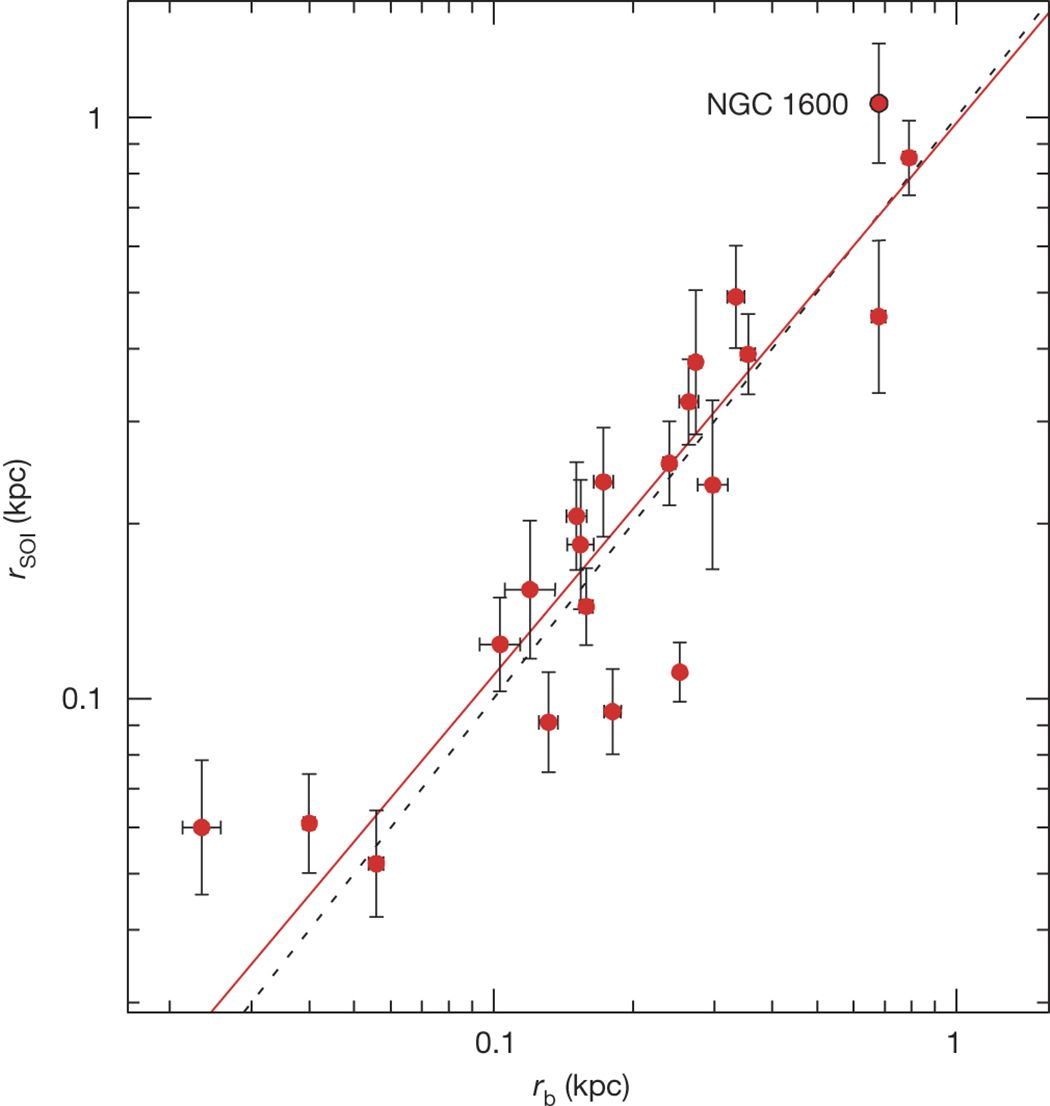
\includegraphics[width=0.7\textwidth]{thomas_mbh-rb.png}
	\caption{Plots of the $M_\bullet$ – $r_b$ relation from equation \ref{eq:m-rb}, alongside the observed values from which the relation has been deduced. The original figure is from \cite{Thomas2016}.}
	\label{figure:m-rb}
\end{figure}

The size of the observed core has also been observed to relate to the mass of the central SMBH of the galaxy. Both simulations and observations have shown that a relation between the central SMBH mass ($M_\bullet$) and the quantity of the observed mass deficit ($M_\mathrm{def}$) exists \citep{Graham2004, Merritt2006, Dullo2014}. Furthermore, there seems to be a relation between the mass of the SMBH and the radius of the depleted core. \cite{Thomas2016}, for example, derive the following scaling relation from observed core sizes and central black hole mass measurements:
\begin{equation}
\log_{10} \left( \frac{M_\bullet}{M_\odot} \right) = (1.17 \pm 0.14) \log_{10} \left( \frac{r_b}{\mathrm{kpc}} \right) + (10.27 \pm 0.51). \label{eq:m-rb}
\end{equation}
Figure \ref{figure:m-rb} shows the above relation alongside observed values for the core radius and the corresponding central black hole mass. While there seems to be quite a bit of scatter between the modelled relation and the observed values, the mass of the central SMBH seems to be connected to the properties of the core. Furthermore, similar relations have been observed by, for example, \cite{Dullo2012}.

\begin{figure}
	\centering
	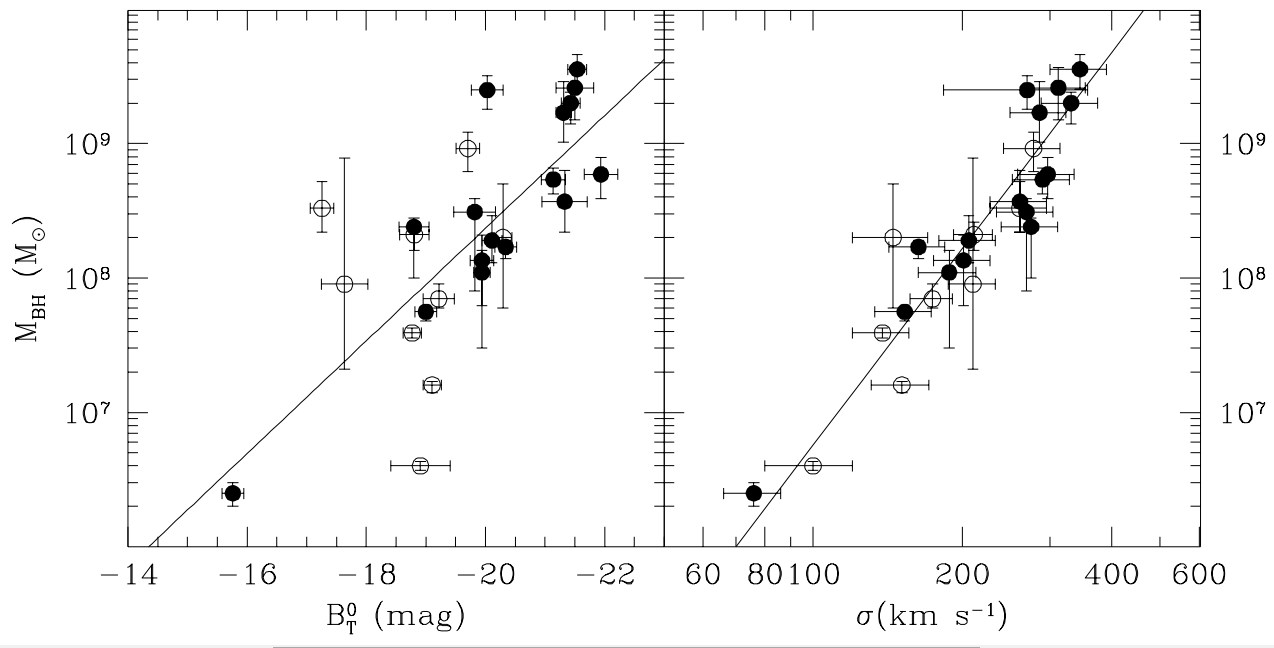
\includegraphics[width=\textwidth]{ferrarese_m-sigma.png}
	\caption{Plots of both the $M_\bullet$ – $L_\mathrm{B,bulge}$ (left) and $M_\bullet$ – $\sigma$ (right) relations, as given by \cite{Ferrarese2005}. The luminosity is given in magnitudes in the plot of the $M_\bullet$ – $L_\mathrm{B,bulge}$ relation, and the relation itself differs somewhat from the one described in equation \ref{eq:m-l_bulge}. The open circles denote observations from the bulges of spiral galaxies, and the filled circles denote observations from elliptical galaxies. The figures are originally from \cite{Ferrarese2005}.}
	\label{figure:m-sigma}
\end{figure}

Though not necessarily proving that the formation of the central SMBH is connected to the development of the core, further evidence that the central black hole is inherently linked to the properties of its host galaxy can be seen in the three main scaling relations of the SMBH mass. These relations include the $M_\bullet - \sigma$ relation \citep{Ferrarese2005}:
\begin{equation}
\frac{M_\bullet}{10^8 \; M_\odot} = (1.66 \pm 0.24) \left( \frac{\sigma}{200 \; \mathrm{km \, s^{-1}}} \right)^{(4.86\pm0.43)}, \label{eq:m-sigma}
\end{equation}
where $\sigma$ is the velocity dispersion; the $M_\bullet - L_\mathrm{bulge}$ relation \citep{Marconi2003}:
\begin{equation}
\log_{10} \left( \frac{M_\bullet}{M_\odot} \right) = (1.13 \pm 0.12) \log_{10} \left( \frac{L_\mathrm{K,bulge}}{L_\mathrm{K,\odot}} \right) + (8.21 \pm 0.07), \label{eq:m-l_bulge}
\end{equation}
where $L_\mathrm{K,bulge}$ is the luminosity of the galactic bulge in $K$-band magnitudes; and the $M_\bullet - M_\mathrm{bulge}$ relation \citep{Marconi2003}:
\begin{equation}
\log_{10} \left( \frac{M_\bullet}{M_\odot} \right) = (0.96 \pm 0.07) \log_{10} \left( \frac{M_\mathrm{bulge}}{M_\odot} \right) + (8.28 \pm 0.06), \label{eq:m-m_bulge}
\end{equation}
where $M_\mathrm{bulge}$ is the mass of the central bulge. Plots for these three relations can be seen in figures \ref{figure:m-sigma} and \ref{figure:m-bulge}. 

The above relations have often been used as evidence for the coevolution of the central black holes and their host galaxies. For example, the $M_\bullet$ – $\sigma$ relation could be \textit{add stuff about BH feedback} However, it is debatable whether this coevolution actually exists \citep{Kormendy2013}.

\begin{figure}
	\centering
	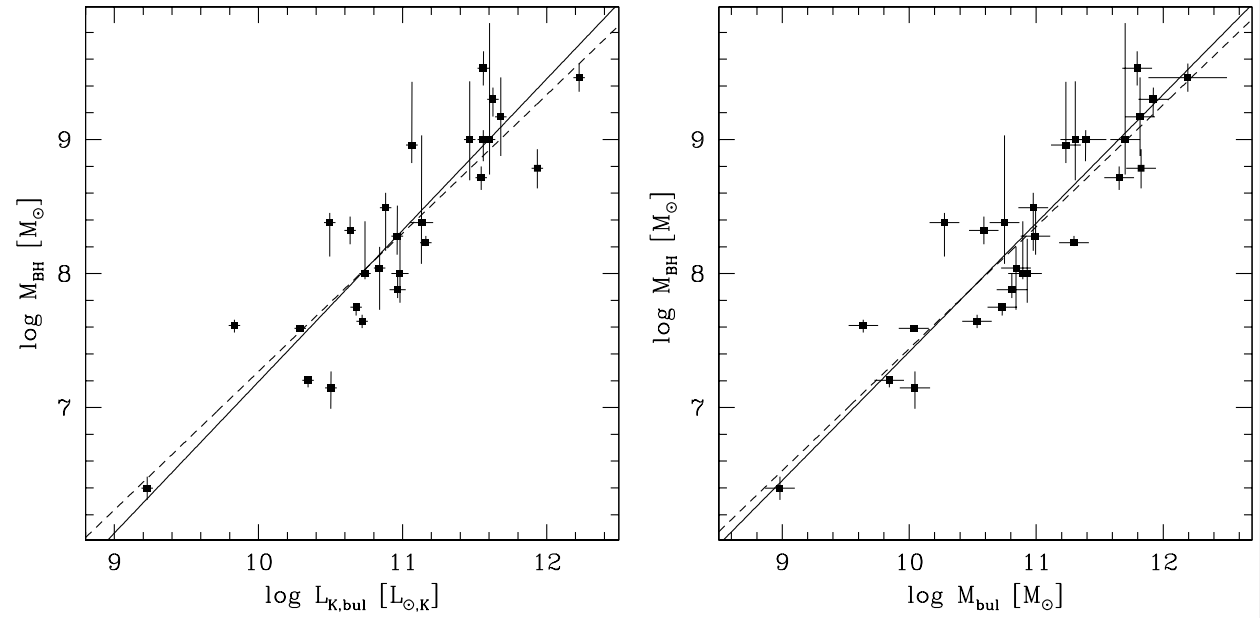
\includegraphics[width=\textwidth]{marconi_m-bul.png}
	\caption{Plots of both the $M_\bullet$ – $L_\mathrm{K,bulge}$ (left) and $M_\bullet$ – $M_\mathrm{bulge}$ (right) relations, with the observed values from which these relations are derived. The solid lines describe the relations given by equations \ref{eq:m-l_bulge} and \ref{eq:m-m_bulge}. The dashed lines are simple "least-squares" fits. The figures are originally from \cite{Marconi2003}.}
	\label{figure:m-bulge}
\end{figure}

\section{Integral-Field Spectroscopy}

Integral-field spectroscopy (IFS) has become an essential part of studying the kinematic properties of ETGs, as it allows for the spatial analysis of galactic spectra. IFS is done using instruments called "integral-field units", which, in principle, calculate the spectrum of the observed light for each pixel. However, often the signal-to-noise ratio ($S/N$) of singular pixels is quite poor. To improve the $S/N$, the pixel measurements are usually combined into so-called "spaxels" (i.e. spatial pixels) using an algorithm, such as the Voronoi-tessellation algorithm \citep{Cappellari2003}. This results in IFU-maps similar to figure \ref{figure:krajnovic_ifus}.

\begin{figure}
	\centering
	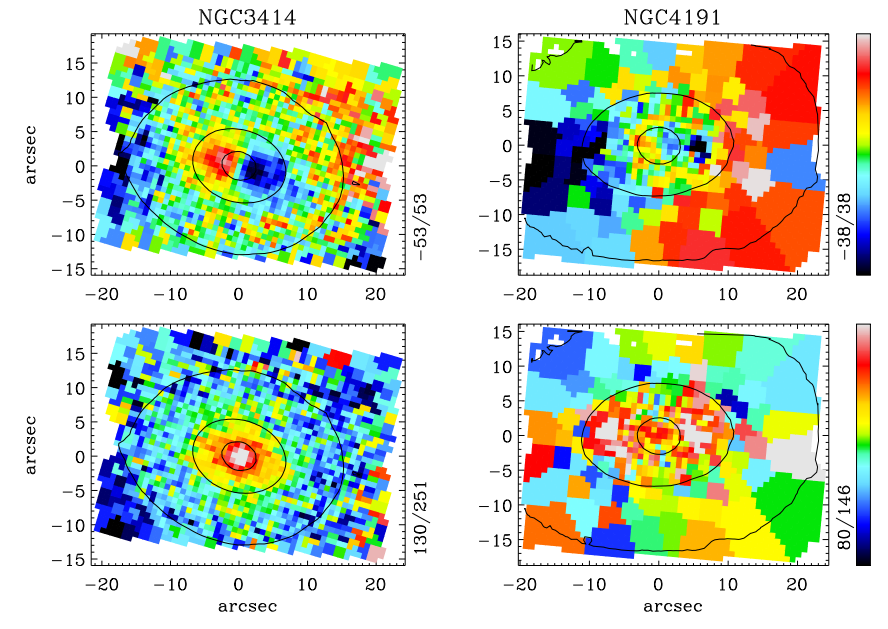
\includegraphics[width=0.9\textwidth]{krajnovic_ifus.png}
	\caption{IFU-maps of the mean line-of-sight velocities (top figures) and line-of-sight velocity dispersions (bottom figures) from the galaxies NGC 3414 and NGC 4191. The figures are originally from \cite{Krajnovic2011}.}
	\label{figure:krajnovic_ifus}
\end{figure}

By creating a histogram out of the observed velocities in the pixels forming a spaxel, the spaxels can show the line-of-sight velocity distribution (LOSVD) of the regions in the observed galaxy that they encompass. The analysis of the LOSVDs is done by fitting the velocity histogram with some theoretical distribution function. Since the LOSVDs are similar to a Gaussian distribution function but rarely purely Gaussian \citep{GalaxyFormationAndEvo2010}, quite often  (e.g. the $\mathrm{SAURON}$ and $\mathrm{ATLAS^{3D}}$ projects, as well as the MASSIVE survey; \citealt{Bacon2001, Cappellari2011, Ma2014MASSIVE}) the fitted distribution function is the following form of the modified Gaussian function \citep{VanDerMarel1993, Bender1994}:
\begin{equation}
f(v) = I_0 e^{-\gamma^2/2}(1 + h_3 H_3(y) + h_4 H_4(y)), \label{eq:mod_gaussian}
\end{equation} 
where $I_0$ is a normalization constant, $\gamma$ is the central slope of the particle density profile, $y = (v - V_\mathrm{avg})/\sigma$, and $H_3$ and $H_4$ are the third and fourth order Hermite polynomials respectively:
\begin{eqnarray}
H_3(y) = \left(2\sqrt{2}y^3 - 3\sqrt{2}y\right) / \sqrt{6}, \\
H_4(y) = \left(4y^4 - 12y^2 + 3 \right) / \sqrt{24}.
\end{eqnarray}
The four remaining parameters: the average LOS velocity $V_\mathrm{avg}$, the LOS velocity dispersion $\sigma$, and the third and fourth order Gauss-Hermite moments $h_3$ and $h_4$, which represent skewness and kurtosis respectively, are usually the parameters that are of interest.

By using IFS, a number of different kinematic features have been observed in ETGs. These features include: areas with low-level velocities or disk-like rotation, as well as regions where the kinematic axis of the galaxy is misaligned with its photometric axis \citep{Emsellem2007}. IFS has also helped identify so-called \textit{Kinematically Distinct Cores} (KDCs), which are central regions of galaxies with angular momentum that has a different direction compared to the rest of its host. There has also been evidence of \textit{Counter Rotating Cores} (CRCs), which are galactic cores that have a difference of around $180^\circ$ in the position angle of their angular momentum vector, when compared to their immediate surroundings \citep{Krajnovic2011}.

\subsubsection{Slow and Fast Rotators}

Using LOSVD measurements done with IFS, \cite{Emsellem2007} have defined an explicit way to classify galaxies as either slow or fast rotators. The basis for this classification is the $\lambda_R$ parameter, which describes the angular momentum of a galaxy, and is defined as:  
\begin{equation}
\lambda_R \equiv \frac{\langle R |V| \rangle}{\langle R \sqrt{V^2 + \sigma^2} \rangle}, \label{eq:general_lambdar}
\end{equation}
where $R$ is the projected distance from the galactic centre, $V$ is the line-of-sight velocity, $\sigma$ is the velocity dispersion and $\langle \; \rangle$ denote that the nominator and denominator in the equation are luminosity weighted means. From binned 2D kinematic maps, such as the ones given by IFS observations, this property can be calculated using the following formula:
\begin{equation}
\lambda_R = \frac{\sum^{N_p}_{i=1} F_i R_i |V_i|}{\sum^{N_p}_{i=1} F_i R_i \sqrt{V_i^2 + \sigma^2_i}}, \label{eq:binned_lambdar}
\end{equation}
where $F_i$, $R_i$, $V_i$ and $\sigma_i$ are the flux, projected distance from the galaxy centre, velocity and velocity dispersion of the $i$th bin, and $N_p$ is the number of bins.

Determining whether a galaxy is a fast or a slow rotator using $\lambda_R$, is done by comparing the value that the parameter gets at the galaxy's effective radius, to some pre-defined threshold. The originally used threshold is: $\lambda_{Re} < 0.1$, where $\lambda_{Re}$ is the aforementioned $\lambda_R$ at the effective radius, and where galaxies fulfilling this condition are classified as slow rotators \citep{Emsellem2007}. A revision of the threshold by \cite{Emsellem2011} takes the ellipticity ($\epsilon$) of the galaxy into account, and defines slow rotators as having $\lambda_{R_e} < 0.31 \sqrt{\epsilon}$, which accounts for the increased anisotropy in the kinematics of flatter galaxies. An even further refinement of the slow rotator definition has been proposed by \cite{Cappellari2016}, where slow rotator galaxies are determined using the following two criteria: $\lambda_{R_e} < 0.08 + \epsilon/4$ and $\epsilon < 0.4$. The former criterion of the threshold reduces the risk of misidentifying very round non-regular slow rotators as fast rotators, while the latter makes sure that only sufficiently round galaxies are classified as slow rotators (\citealt{Cappellari2016} argues that "genuine" disk-less slow rotators are all rounder than $\epsilon = 0.4$).

Slow rotator galaxies, when defined using the above methods, often contain a KDC, and usually exhibit: anisotropic velocity distributions, little to no large-scale rotation, kinematic misalignments and twists \citep{Emsellem2007, Cappellari2007}. In contrast, the velocity distributions of fast rotators are isotropic and their kinematic axis is aligned closely with their photometric axis \citep{Emsellem2007}. They also have disk-like kinematics and nearly oblate shapes \citep{Cappellari2007}. 

As expected, the dichotomy between slow and fast rotators clearly mirrors the kinematic differences between "boxy" and "disky" ellipticals. This implies that the cored and coreless galaxies should follow the slow and fast rotator divide as well. \cite{Krajnovic2013} find that this indeed does seem to be the case, however there are a few exceptions. Nevertheless, even when accounting for these exceptions, \cite{Cappellari2016} for example, consider the agreement to be good enough, that it is possible to adequately draw conclusions about the photometry or kinematics of these galaxies.

\section{Galactic Dynamics}

\subsection{Collisional And Collisionless Systems}

The movement of stars in stellar systems is caused by gravitational forces. However, when modelling the motion of stars in systems with a large stellar population, it is often appropriate to ignore the changes to their orbits caused by specific stellar encounters, and simply approximate their motion as being caused by a smooth continuous gravitational potential. Systems where this approximation is applicable are called "collisionless systems", where as systems where the modelling of the stellar motion requires knowledge about the gravitational effects caused by distinct massive particles, are called "collisional systems".

Whether a stellar system can be approximated as collisionless is determined by its age, but it is also affected by the number of particles it contains. There are two conditions that must be met for the approximation to be valid: the stars must be uniformly distributed in the system, so the age of the system must be older than the orbital period of a star; and the system must be younger than its relaxation time (explained below) \citep{MerrittBook}. Usually, it is the latter of these conditions that is of interest.

Relaxation time is the time it takes, for the cumulative effect of encounters between a subject star and multiple field stars, to change the orbit of the subject star in such a significant way, that its initial conditions can not be inferred from its current motion. This process is often called "two-body relaxation". The relaxation time itself can be calculated using the following formula \citep{BinneyTremaine}:
\begin{equation}
t_\mathrm{relax} \simeq \frac{0.1N}{\ln N} t_\mathrm{cross},
\end{equation}
where $N$ is the number of particles in the system, and $t_\mathrm{cross}$ is the crossing time, which is defined as the time it takes for a typical field-star to cross the system once, and the value of which can be estimated using the radius of the system $R$ and the typical field-star velocity $v$ as $t_\mathrm{cross} = R/v$. 

Of specific interest to collisionless systems is the concept of "phase space", as it allows one to model the general motion in stellar systems while neglecting the calculation of the motion of distinct stars. Phase space itself is simply an expansion of the basic three-dimensional position space, which enables one to describe each specific state of a system as a point in a higher-dimensional space. In the case of galactic dynamics, it is useful to describe the states of stars as being points in the six-dimensional position-velocity phase space, which contains three physical position coordinates ($x, y, z$) and three velocity coordinates ($v_x, v_y, v_z$). If all stars in the system have identical masses, these six dimensions can describe every dynamical state that a star can have, and thus the state of the whole stellar system at a certain time $t$ can be described using the stellar distribution function $f(\mathbf{x}, \mathbf{v}, t)$, which is also known as the phase space density. The time-dependent behaviour of the system can then be modelled using the "collisionless Boltzmann equation":
\begin{equation}
\frac{\partial f}{\partial t} + \mathbf{v} \cdot \nabla f - \nabla \phi \cdot \frac{\partial f}{\partial \mathbf{v}} = 0,
\end{equation}
where $\phi$ is the gravitational potential of the system, and which states that the phase space density is conserved around a particle moving in the phase space.

\subsection{Potential-Density Models}

In order to use the "collisionless system"-approximation to model stellar motion in galaxies, knowledge about their gravitational potential is fundamental. If the mass-density distribution of the galaxy is known, the corresponding potential can be calculated from the Poisson's equation \citep{BinneyTremaine}:
\begin{equation}
\nabla^2 \phi = 4 \pi G \rho, \label{eq:poisson}
\end{equation}
where $\phi$ is the gravitational potential, $G$ is the gravitational constant, and $\rho$ is the aforementioned mass-density distribution. Different types of galaxies can, of course, have different mass distributions, which leads us to the so-called "potential-density models". These models describe galaxies using different density distributions, and then calculate their corresponding gravitational potential using the Poisson's equation. The initial mass-density distribution in the models is often derived in such a way that it is able to account for properties observed in actual galaxies (e.g. the Dehnen model described below). 


One of the most popular potential-density models used when approximating elliptical galaxies, is the spherically symmetric Dehnen-model \citep{Dehnen1993}, which is defined as:
\begin{equation}
\rho(r) = \frac{(3-\gamma)M}{4\pi} \frac{a}{r^\gamma (r+a)^{4-\gamma}}, \label{eq:dehnen_density}
\end{equation}
\begin{equation}
\phi(r) = \frac{GM}{a} \times 
\begin{cases}
	-\frac{1}{2-\gamma} \left[ 1 - \left( \frac{r}{r+a} \right)^{2-\gamma} \right] & \; \gamma \neq 2 \\
	\ln \frac{r}{r+a}	 & \; \gamma = 2
\end{cases},
\label{eq:dehnen_potential}
\end{equation}
where $M$ is the total mass, $a$ is the scaling radius, and $\gamma$ is the central slope of the profile. There are a few reasons why this model in particular is used often. Firstly, the density profile is a combination of two power-laws. This is similar to many observed luminosity and surface brightness profiles in Es (see section \ref{section:ellip_photo}), and also many simulated dark-matter profiles \citep{BinneyTremaine}. Furthermore, when projected, the outer parts of the density profile resembles the empirical "de Vaucouleurs" surface brightness profile. The model is also a generalization of two other commonly used potential-density models, namely the Jaffe-model and the Hernquist-model \citep[for these models $\gamma = 2$ and $\gamma = 1$ respectively][]{Jaffe1983, Hernquist1990}. 

\section{Regularization}

The nature of elliptical galaxy mergers and the formation of merger remnants with cores deficient in light, is such, that simulations of the process must take into account strong interactions between stars and black holes. This leads to a common issue encountered in simulations of collisional systems, namely the singularity at $r=0$ in the equation of motion \citep{BinneyTremaine}:
\begin{equation}
\ddot{r} = -GM/r^2, \label{eq:equation_of_motion}
\end{equation}
where $G$ is the gravitational constant, $M$ is the total mass of the two interacting particles, and $r$ is the distance between the particles. Often, when calculating the orbits of stars, these simulations maintain accuracy by shortening the integration time-step when the accelerations of the objects become large. On extremely close encounters, the singularity in equation \ref{eq:equation_of_motion} causes the accelerations of the objects to rise sharply, resulting in smaller and smaller time steps, effectively stopping the simulation time from progressing. 

The solution to the above issue is so-called regularization, where the singularity in the equation of motion (equation \ref{eq:equation_of_motion}) is removed through a coordinate transformation. Two examples of such transformations are given by \cite{BinneyTremaine}. The first is the "Burdet-Heggie regularization", which adds the gravitational field of the other particles to the two-body problem, and changes the simulation time to the fictitious time: $\mathrm{d}t = r \; \mathrm{d}\tau$. 

\begin{figure}
	\centering
	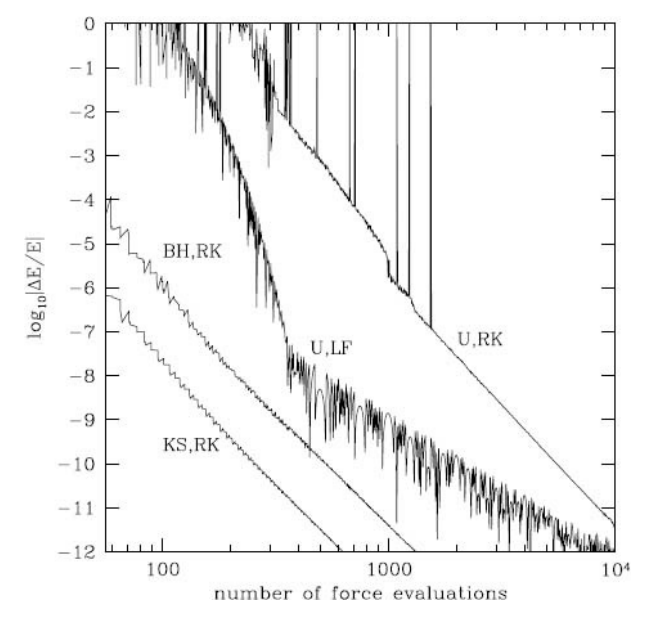
\includegraphics[width=0.7\textwidth]{binneytremaine_pic.png}
	\caption{Fractional error of the energy of an orbit with an eccentricity of $e=0.99$, as a function of the number of force calculations per orbit. The errors were calculated after a single pericentre passage of the orbiting object. The multiple graphs denote errors produced by different integrators and regularization procedures. \textit{U}, \textit{BH} and \textit{KS} denote unregularized, "Burdet-Heggie" and "Kustaaheimo-Stiefel" regularizations, respectively. \textit{RK} and \textit{LF} denote "Runge-Kutta" and "Leapfrog" integrators (both defined in the next-section), respectively. The figure is originally from \cite{BinneyTremaine}.}
	\label{figure:regularized}
\end{figure}

The second one is the "Kustaaheimo-Stiefel" (KS) regularization, which converts the equation of motion of the two-body problem, into an equation of motion similar to that of a harmonic oscillator, by transforming the three-dimensional spatial coordinates into four-dimensional coordinates. Like the Burdet-Heggie regularization, KS-regularization defines a new fictitious time $\mathrm{d}t = r \; \mathrm{d}\tau$ and adds the gravitational field of the other particles to the equation of motion. The spatial coordinate transformation is done by changing the position vector $\mathbf{r} = (x, y, z)$ into a corresponding four-vector $\mathbf{u} = (u_1, u_2, u_3, u_4)$, where:
\begin{align}
\begin{split}
u_1^2& = \frac{1}{2}(x+r)\cos^2\psi \\
u_2^2& = \frac{yu_1+zu_4}{x+r} \\
u_3^2& = \frac{zu_1+yu_4}{x+r} \\
u_4^2& = \frac{1}{2}(x+r)\sin^2\psi,
\end{split}
\end{align}
and where $\psi$ is some arbitrary parameter \citep{BinneyTremaine}. If $\phi_e$ is the gravitational potential induced outside the particles outside the two-body problem, the equation of motion becomes as follows:
\begin{equation}
\mathbf{u}'' - \frac{1}{2} E \mathbf{u} = -\frac{1}{4} \frac{\partial}{\partial\mathbf{u}} \left( |\mathbf{u}|^2 \phi_e \right), \label{eq:ks_motion}
\end{equation} 
where $\mathbf{u}''$ denotes the second fictional time derivative of the four-vector, and $E$ is the energy of the two-body orbit when $\phi_e$ is taken into account:
\begin{equation}
E = \frac{1}{2}v^2 - \frac{GM}{r} + \phi_e = 2 \frac{|\mathbf{u'}|^2}{|\mathbf{u}|} - \frac{GM}{|\mathbf{u}|^2} + \phi_e.
\end{equation}
Equation \ref{eq:ks_motion} is now the equation of motion of a four-dimensional harmonic oscillator with an added external force \citep{BinneyTremaine}. Furthermore, as the equation in question clearly shows, the regularized form of the equation of motion is well defined even when the new position vector gets the value $\mathbf{u} = 0$, and thus does not contain the same singularity as the basic Cartesian version in equation \ref{eq:equation_of_motion}.

Figure \ref{figure:regularized} by \cite{BinneyTremaine} compares the fractional errors in the energies of highly eccentric simulated orbits ($e = 0.99$), integrated in differently regularized (or non-regularized) coordinates, after one pericenter passage. The figure clearly shows how important the removal of the singularity is for the accuracy of the integration of the orbit. In regularized coordinates, the integrators require around an order of magnitude less force evaluations to achieve the same accuracy than in unregularized coordinates. Furthermore, the efficiency of the integration seems to also be affected by the type of regularization, as the more robust KS-regularization results in a smaller fractional energy error as the Burdet-Heggie regularization.

\section{Post-Newtonian Dynamics}

When simulating mergers of galaxies that contain central SMBHs, general relativity has to be taken into account, as relativistic effects not only affect the orbits of stars that pass close to the black holes significantly, but are also required for the formation of the gravitational waves that drive the coalescence of the SMBH binary during the final stage of its merger. However, since the equations that describe these effects are difficult to solve, and thus inefficient to use in simulations; they are often approximated using so-called "Post-Newtonian" (PN) dynamics.

PN dynamics are an extension of the basic Newtonian dynamics that approximates the effects that Einstein's general theory of relativity has in two-body encounters, by adding so-called PN-terms to the Newtonian equation of motion. This results in an equation of motion similar to:
\begin{equation}
\mathbf{a} = \mathbf{a}_\mathrm{Newtonian} + \mathbf{a}_\mathrm{1PN} + \mathbf{a}_\mathrm{2PN} + \mathbf{a}_\mathrm{2.5PN} + \ldots, \label{eq:PN_eom}
\end{equation}
where $\mathbf{a}_\mathrm{Newtonian}$ is the acceleration from the basic Newtonian equation motion, and $\mathbf{a}_\mathrm{xPN}$ are added PN corrections with values of the degree of $\mathbf{a}_\mathrm{xPN} \propto (v^2/c^2)^x$. 

The formulae for the PN-terms are quite long, and are thus not given here. However, they are derived from the expansion of Einstein's equations based on the two approximations that: the objects are assumed to be point masses, and that the equation \citep{MerrittBook}:
\begin{equation}
\left( \frac{v}{c} \right)^2 \approx \frac{Gm}{c^2r} \ll 1,
\end{equation}
where $G$ is the gravitational constant, $c$ is the speed of light, $m$ is the total mass of the two interacting particles, and $v$ and $r$ are the relative velocity and distance between the particles respectively, holds true. In words, the above equation means that the velocities of the moving objects are assumed to be of the order that is expected for gravitaionally bound systems, and thus significantly slower than the speed of light, and that the objects are never brought near the gravitational radius of one another \citep{MerrittBook}. 

An important caveat to note is that, the point mass assumption of the PN approximation ignores the relativistic effects that the spin of the black hole, alongside its non-spherical shape, has on closely orbiting objects. The effects caused by the spin of the black hole include orbital precession (i.e. changes in the rotational axis of the orbit), as well as precession of the spin itself \citep{Kidder1995}. The lack of spherical symmetry in the shape of the BH, on the other hand, results in additional non-radial acceleration for the orbiting object \citep{MerrittBook}. These effects can, however, be taken into account by including an additional spin PN-term in the equation of motion (equation \ref{eq:PN_eom}).

Depending on the degree, a PN-term either describes an effect that conserves the energy of the system, or an effect where energy is dissipated through gravitational radiation in the form of gravitational waves \citep{Mora2004}. Terms that have a degree that is an integer are conservative, while the half-degree terms are radiative and cause the orbit of a two-body system to shrink. For this reason, when simulating black hole mergers, it is imperative to include terms upto at least 2.5PN in the equation of motion.

\chapter{KETJU}

\textit{Description of basic functionality: what KETJU does, why it's created, basic description of the multiple integration region system.} 

\section{AR-CHAIN / Chain Integrator}

\textit{Chain forming, force calculations, integration}

\section{GADGET-3 / Tree Integrator}

\textit{Softening, tree-codes, calculations}

\section{Combined Functionality}

\textit{How the AR-CHAIN and GADGET-3 integrators work together: time-step problem, tidal-perturbations, particles moving from one region to another, chain macro-particle}

\subsection{Particle Types}

\textit{Chain particles, tree particles, perturber particles}

\section{Merging of Black Hole Particles}

Since we are trying to determine if merging SMBH binaries form cores in merger remnants, we must make sure that the progenitors' central black holes actually merge in our simulations. This is done by looking at the "Run" simulations, as they contain the locations of the black holes from multiple time steps, and as the "Snapshots" still show both of the SMBHs.

Plotting the positions of the black holes from "Run 3" in coordinates centred on the binary's centre-of-mass during the initial time step gives us figure \ref{figure:run3_traj}. Even by eye, one can clearly see that the orbit of the black hole with a smaller mass becomes smaller and smaller as the binary moves further away from its initial position. While this doesn't explicitly tell us that the black holes merge into each other, it does indicate the existence of a hardening process in the binary. Similar figures to figure \ref{figure:run3_traj} from all four "Runs" can be found in the appendix (figure \ref{figure:all_traj}).

\begin{figure}[h]
	\centering	
	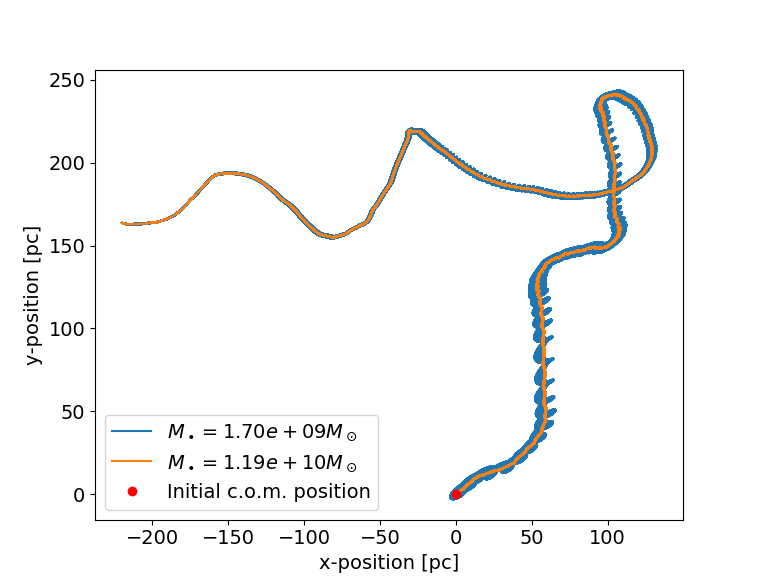
\includegraphics[width=0.7\textwidth]{Run3_Trajectory.png}	
	\caption{The trajectories of the black holes during "Run 3". The coordinates are centred on the initial location of the centre-of-mass of the binary black hole. The orange and blue lines show the paths taken by the smaller and larger black holes respectively. Both paths show clear spiral patterns which become smaller and smaller as the simulation proceeds. The paths end at the location where the black holes merge, i.e. where the distance between them is $\lesssim 100 R_s$ ($R_s$ is the Schwarzschild radius).}
	\label{figure:run3_traj}
\end{figure}

\begin{figure}[h]
	\centering
	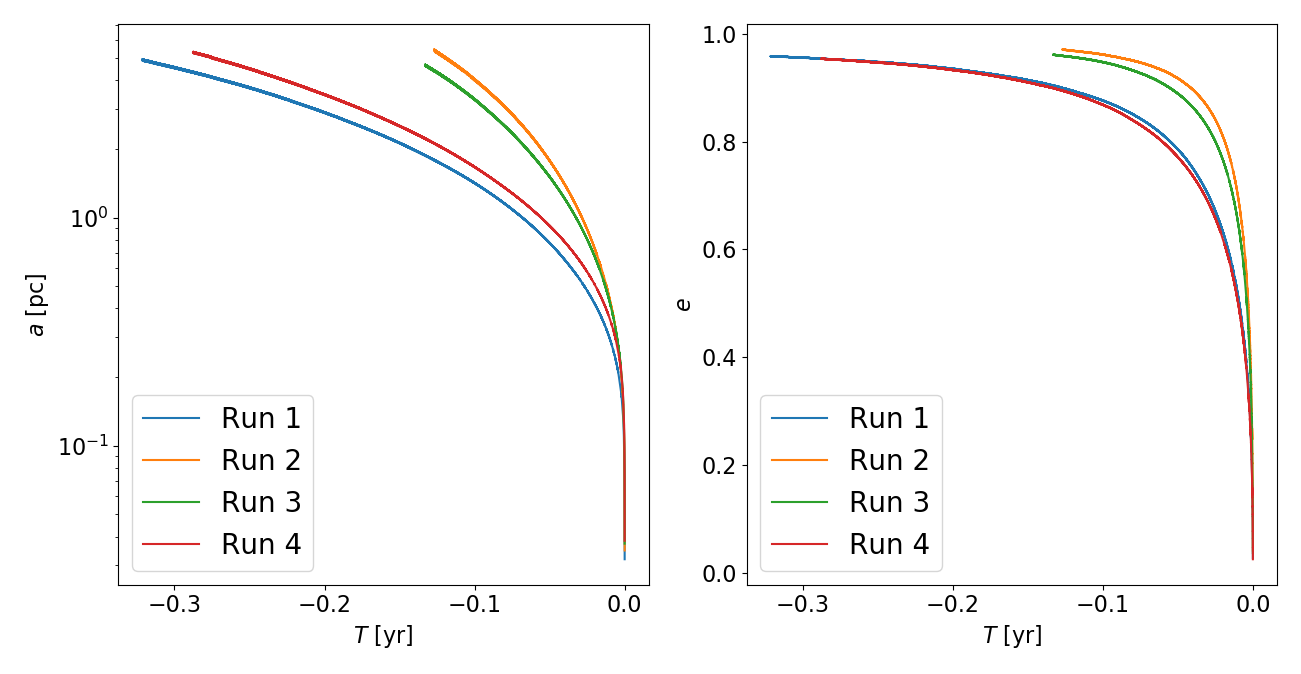
\includegraphics[width=\textwidth]{semi_major_and_ecc.png}
	\caption{The semi-major axes (left) and eccentricities (right) of the black hole systems in the simulations "Runs 1"-"Run-4" as a function of time. The zero position on the x-axis corresponds to the point in simulation time, where the black hole merging event occurs.}
	\label{figure:semi_and_ecc}
\end{figure}

The most likely obstacle for the complete merging of the binary black holes is the so-called final-parsec problem; where, due to the lack of stellar material that can be ejected during the three-body scattering phase, the hardening of the binary stops when the separation between the two black holes is $\sim 1 \mathrm{pc}$. This is assumed to happen since, not only is the binary constantly ejecting the finite amount of stars inside the loss-cone (defined in section 2), but the loss cone itself is becoming smaller due to the contracting binary orbit.

Figure \ref{figure:semi_and_ecc} shows the time evolution of both the semi-major axis and the eccentricity of the binary orbits from all of the simulation runs. Interestingly enough the semi-major axes of all of the binaries go far below single parsec scales, meaning that the final-parsec problem doesn't seem to play a part in the simulations. This implies that, there exists some loss-cone refill mechanism which allows the binary to eject more stellar material than what initially exists inside the loss cone.



\chapter{Merger Simulations Using KETJU}

In this chapter I study the formation of cored galaxies in galaxy mergers. The analysis focuses on the results from galaxy merger simulations run by \cite{Rantala2018} using the KETJU code. In all but one simulation, the merger progenitor galaxies contain central supermassive black holes. During the merger event the SMBHs form a hard binary. These binaries are a likely source for the observed low-luminosity cores, as they can eject stars from the galactic centre through complex three-body interactions. Here I determine if there is a connection between the central binary SMBH and the existence of a core deficient in light, and if the simulated KETJU results agree with observations of cored galaxies.


\section{Simulation Details}

The simulation sample run by \cite{Rantala2018} includes seven different equal-mass mergers of two identical galaxies. The merger progenitor galaxies (named BH-0 - BH-6) used in the different simulations consist of equal mass stellar particles and equal mass dark matter particles, where the mass of the stellar particles differ from the mass of the dark matter particles. The progenitors are gas free (i.e. the simulations describe so-called "dry" mergers), and all of them but one contains an SMBH at their centre.

The initial conditions (ICs) of the merger progenitor galaxies are modelled as multicomponent, spherically symmetrical stellar systems. They consist of the three aforementioned components: stellar particles, dark matter particles and a central SMBH. The central SMBH is simply modelled as a single point mass, and is located at the origin of the host galaxy's internal coordinate systems. The stellar and dark matter component, on the other hand, consist of multiple particles which are distributed according to the spherically symmetric Dehnen density-potential model defined as \citep{Dehnen1993}:
\begin{equation}
\rho(r) = \frac{(3-\gamma)M}{4\pi} \frac{a}{r^\gamma (r+a)^{4-\gamma}}, 
\end{equation}
\begin{equation}
\phi(r) = \frac{GM}{a} \times 
\begin{cases}
	-\frac{1}{2-\gamma} \left[ 1 - \left( \frac{r}{r+a} \right)^{2-\gamma} \right] & \; \gamma \neq 2 \\
	\ln \frac{r}{r+a}	 & \; \gamma = 2
\end{cases},
\end{equation}
where $M$ is the total mass, $a$ is the scaling radius, and $\gamma$ is the central slope of the profile. For stellar particles we set $\gamma = 3/2$, while for the dark matter particles the value of $\gamma = 1$ is used ($\gamma = 1$ corresponds to the so-called Hernquist profile, \citealt{Hernquist1990}). The Dehnen density-potential model uses a density profile, which is a generalization of stellar density models that, when projected, resemble the de Vaucouleurs - profile \citep[$\log(\mu) \propto R^{1/4}$;][]{deVaucouleurs1948} in the outer parts. The model's gravitational potential profile is derived from the density profile using the Poisson equation \textit{(refer to equation from chapter 2)}. 

When constructing the multicomponent ICs for the progenitor galaxies, the positions of the stellar and dark matter particles are determined through their respective cumulative mass profiles. These mass profiles are derived using the aforementioned Dehnen density-potential model, and can be written as:
\begin{equation}
M(r) = 4\pi \int^r_0 \rho(r)r^2 \;dr = M \left( \frac{r}{r+a} \right)^{3-\gamma}, \label{eq:cumulative_mass}
\end{equation}
where $\rho(r)$ is the density profile from equation \ref{eq:dehnen_density}.

In equation \ref{eq:cumulative_mass}, the value of the scaling radius ($a$) is determined quite differently for the stellar and dark matter particle distributions. One way of calculating $a$ is to derive the formula for the half-mass radius from the cumulative mass profile. This gives us the equation:
\begin{equation}
r_{1/2} = a \left( 2^{1/(3-\gamma)}-1 \right)^{-1}, \label{eq:half-mass-radius}
\end{equation}
from which $a$ can be solved easily. However, in order to get a value for $a$, one now needs to know the half-mass radius of the particle distribution. Fortunately, the half-mass radius of the stellar population can be determined through drawing an equivalence between it and the effective radius of the galaxy. If the galaxy for which we are trying to determine the scaling radius has a constant mass-to-light ratio, its mass and light profiles are proportional to each other. In this case, both profiles describe the same property, which means that the half-mass radius and the effective radius are equivalent to each other. In cases, such as our simulations, where only the 2D projection of the effective radius is known, the three dimensional half-mass radius can be approximated using the following formula:
\begin{equation}
R_e \approx \frac{3}{4} r_{1/2}, \label{eq:projection_approximation}
\end{equation} 
where $R_e$ is the aforementioned 2D projected effective radius. Thus, knowing the effective radius of the galaxy allows one to determine the stellar scaling radius $a_\star$, by using both equation \ref{eq:half-mass-radius} and \ref{eq:projection_approximation}.

The scaling radius of the dark matter particle distribution can be derived using the dark matter fraction ($f_{\mathrm{DM}}$) inside the stellar half-mass radius. The dark matter fraction describes the fraction of the total mass inside radius $r$ that is contributed by dark matter, and is defined by the following equation:
\begin{equation}
f_\mathrm{DM}(r) = \frac{M_\mathrm{DM}(r)}{M_\star(r) + M_\mathrm{DM}(r)}. \label{eq:dm_fraction}
\end{equation}
With the above equation, one can get the dark matter scaling radius by substituting the cumulative mass profiles in the equation with the one from equation \ref{eq:cumulative_mass} when $r=r_{1/2}$, and using equation \ref{eq:half-mass-radius} to define the stellar half-mass radius. This gives us the following formula for calculating the dark matter scaling radius:
\begin{equation}
a_\mathrm{DM} =  r_\mathrm{1/2} \left[ \sqrt{\frac{2M_\mathrm{DM}}{M_\star} \left( \frac{1}{f_\mathrm{DM}(r_{1/2})} - 1 \right)} -1 \right].
\end{equation}
Finally, applying the half-mass radius approximation from equation \ref{eq:projection_approximation} allows us to calculate the dark matter scaling radius as follows:
\begin{equation}
a_\mathrm{DM} \approx \frac{4}{3} \left[ \sqrt{\frac{2M_\mathrm{DM}}{M_\star} \left( \frac{1}{f_\mathrm{DM}(r_{1/2})} - 1 \right)} -1 \right] R_e.
\end{equation}

If the positions of the particles in the simulated progenitor galaxies are known, their velocities can be determined using Eddington's formula \citep{BinneyTremaine}. The different particles thus have the following distribution function in the position-velocity phase-space:
\begin{equation}
f_i(\varepsilon) = \frac{1}{\sqrt{8}\pi^2} \int^{\Phi_T = \varepsilon}_{\Phi_T = 0} \frac{d^2\rho_i}{d\Phi^2_T}
\frac{d\Phi_T}{\sqrt{\varepsilon - \Phi_T}}, \label{eq:eddington_form}
\end{equation}
where $\rho_i$ is the density profile from equation \ref{eq:dehnen_density} for the particle in question, and $\Phi_T$ is the total gravitational potential ($\Phi_T = \Phi_\star + \Phi_\mathrm{DM} + \Phi_\bullet$). The variable $\varepsilon$ is the relative energy:
\begin{equation}
\varepsilon = -\Phi_T + \Phi_0 - \frac{1}{2} v^2,
\end{equation}
where $v$ is the velocity of the particle, and $\Phi_0$ is a chosen zero point for the potential. This zero point is usually chosen so that, $f > 0$ for $\varepsilon > 0$, and that $f = 0$ for $\varepsilon \leq 0$. In the case of our simulations the zero point is set as $\Phi_0 = 0$, since the galaxies are modelled in isolation, and extend in principle to infinity.

The general procedure for generating the multicomponent ICs of the progenitor galaxies is as follows. The positions of the stellar and dark matter particles are generated using the inverse of their respective cumulative mass function described in equation \ref{eq:cumulative_mass}. Afterwards, using equation \ref{eq:eddington_form}, values of the two particle types' distribution functions are calculated into a lookup table. The velocities of the particles are then sampled by interpolating these tabulated distribution function values. Finally, the central SMBH is placed in the centre of the progenitor galaxy.

The physical parameters needed for generating the progenitor galaxies using the aforementioned procedure are given in table \ref{table:properties} under "Common physical properties". As the name implies, they are identical across every progenitor galaxy used in the simulations; meaning that, as far as their stellar and dark matter particle populations go, the progenitors are identical. 

The values for these common properties are motivated by observations and dynamical simulations of NGC 1600 \citep{Rantala2018}. NGC 1600 is a massive ($M_\star \approx 8.3 \times 10^{11} M_\odot$) early-type cored galaxy with a large observed core radius ($r_b \approx 2.15 \; \mathrm{arcsec}$, which corresponds to a physical length of $\sim 0.667 \; \mathrm{kpc}$ at the distance of $64 \; \mathrm{Mpc}$) and a central supermassive black hole with a mass of $\sim 1.7 \times 10^{10} M_\odot$ \citep{Thomas2016}. Using the values given in table \ref{table:properties} for the physical properties of the simulated merger progenitors, the resulting merger remnant should in principle be as similar as possible to NGC 1600.

Figure \ref{figure:IC_density_profile} shows an example of what the stellar mass density profiles of the merger progenitors used in the simulation look like. The profile is calculated from a stellar particle distribution produced using the multicomponent IC generation procedure described previously in this section. The physical properties used in the generation of the distribution are mostly the same as the ones seen in table \ref{table:properties}. The only difference being that the number of stellar and dark matter particles is only $10 \%$  of the values seen in the table. The density profile itself is calculated by moving the stellar particles of the progenitor galaxy into their centre-of-mass coordinates, dividing them into logarithmic bins, and calculating the mass density inside the respective bins.

\begin{table}
	\begin{center}
		\begin{tabular}{| c c c c c c c |}
		\hline
		\multicolumn{7}{|c|}{Common physical properties} \\
		\hline
		$M_\star$ & $R_e$ & $M_\mathrm{DM}$ & $f_\mathrm{DM}(r_{1/2})$ & $N_\star$ & $N_\mathrm{DM}$ & \\
		$[\times 10^{10} M_\odot]$ & $\mathrm{[kpc]}$ & $[\times 10^{10} M_\odot]$ & & & & \\
		$41.5$ & $7$ & $7500$ & $0.25$ & $4.15 \times 10^6$ & $1.0 \times 10^7$ & \\
		\hline
		\hline
		\multicolumn{7}{|c|}{$M_\bullet$ $[\times10^{9} M_\odot]$} \\
		\hline
		BH-0 & BH-1 & BH-2 & BH-3 & BH-4 & BH-5 & BH-6 \\
		- & $0.85$ & $1.7$ & $3.4$ & $5.1$ & $6.8$ & $7.5$ \\
		\hline
		\end{tabular}
	\end{center}
	\caption{Physical properties of the different progenitors used in the simulations by \cite{Rantala2018}. \\
	$M_\star$: Stellar mass \\
	$R_e$: 2D projected Effective radius \\
	$M_\mathrm{DM}$: Dark matter halo mass \\
	$f_\mathrm{DM}(r_{1/2})$: The fraction of dark matter mass from the total mass inside the half-mass radius \\
	$N_\star$: Number of stellar particles \\
	$N_\mathrm{DM}$: Number of dark matter particles \\
	$M_\bullet$: Central SMBH Mass}
	\label{table:properties}
\end{table}

Table \ref{table:properties} also shows the masses of the central SMBHs in each of the seven progenitor galaxies. The mass of the central SMBH is the only physical property that changes from one progenitor to another. Six of the progenitor galaxies (BH-1 - BH-6) contain central supermassive black holes, with the SMBH masses varying from $8.5 \times 10^8 M_\odot$ to $8.5 \times 10^9 M_\odot$. A merged binary of two of the largest SMBHs in the table, is equivalent in mass to the observed central SMBH in NGC 1600. The seventh progenitor (BH-0) does not contain an SMBH in its centre, and is included simply for the sake of comparison.

\begin{figure}
	\centering
	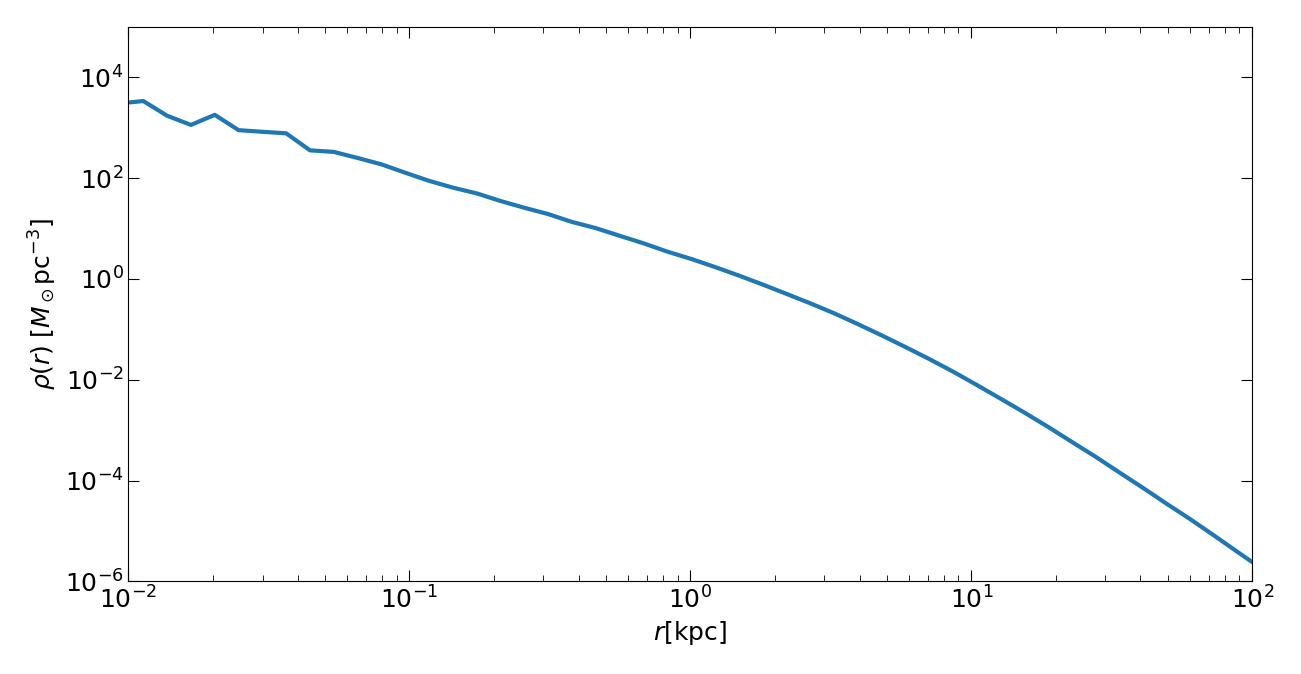
\includegraphics[width=\textwidth]{IC.png}
	\caption{Example mass density profile of the progenitor galaxies. The initial conditions for the profile in question were the same as in table \ref{table:properties}; with the exception of the number of dark matter and stellar particles, which were only $10\%$ of their respective values. The noise in the left-side of the profile is caused by this low particle sample.}
	\label{figure:IC_density_profile}
\end{figure}

The simulations themselves thus comprise of seven mergers of two identical progenitor galaxies from table \ref{table:properties}. The galaxies are merged on a nearly parabolic orbit with an initial separation of $d = 30 \; \mathrm{kpc}$. This kind of orbit makes the approach of the galaxies swift, and causes the stellar cusps to merge before $t \sim 300 \; \mathrm{Myr}$.

The simulation data that I will be analysing, comes in the form of snapshots of the merger remnants. These snapshots are taken at the simulation time of $\sim 2 \mathrm{Gyr}$. At this point the progenitor galaxies have merged into a single merger remnant, however, the progenitors' central SMBHs have not yet merged and still exist in the form of a central binary. The snapshots contain the positions, velocities and masses of every particle.

\section{Core Size Measurements}

In order to test if a galaxy is cored, I calculate its surface brightness profile and check if the centre of the galaxy is deficient in light.

The surface brightness profiles are calculated from the merger remnant snapshots using the following procedure. First, the coordinate system is changed to centre-of-mass coordinates, and the stellar particles are projected onto a 2D plane. Next, we calculate the mass inside logarithmically spaced radial bins, and get a radial surface mass density profile. This is repeated 100 times from random viewing angles, which naturally results in 100 slightly different density profile projections. These profiles are then averaged azimuthally, which results in a smooth surface mass density profile. Finally, by assuming a mass-to-light ratio for the stellar particles, the surface mass density profile can be turned into a surface brightness profile \citep{Rantala2018}. 

Determining the mass-to-light ratios of the stellar particles in the simulated merger remnants is problematic, as the simulations do not contain information about their ages and metallicities. The only properties that the stellar particles have are their position, velocity, and a mass that is identical for all of them; which are not enough to make valid, physically accurate, assumptions on their specific mass-to-light ratios. For this reason, a constant mass-to-light ratio of $M/L = 4$ is used. This is equivalent to the ratio derived from dynamical modelling of NGC 1600 by \cite{Thomas2016}. Thus, the use of this particular $M/L$ in the analysis of the simulation results, fits in well with the already established desire of similarity between the physical properties of the simulated merger remnants and NGC 1600.

Figure \ref{figure:surface_brightness} shows the surface brightness profiles of every simulated merger remnant. Studying the curves, one can already see that, the presence of central SMBHs in the merger progenitors causes a clear brightness deficiency near the centre of the merger remnant. In addition, there is a systematic effect which shows that the larger the mass of the central black hole binary, the larger the amount of missing light in the core.

\begin{figure}[h]
	\centering
	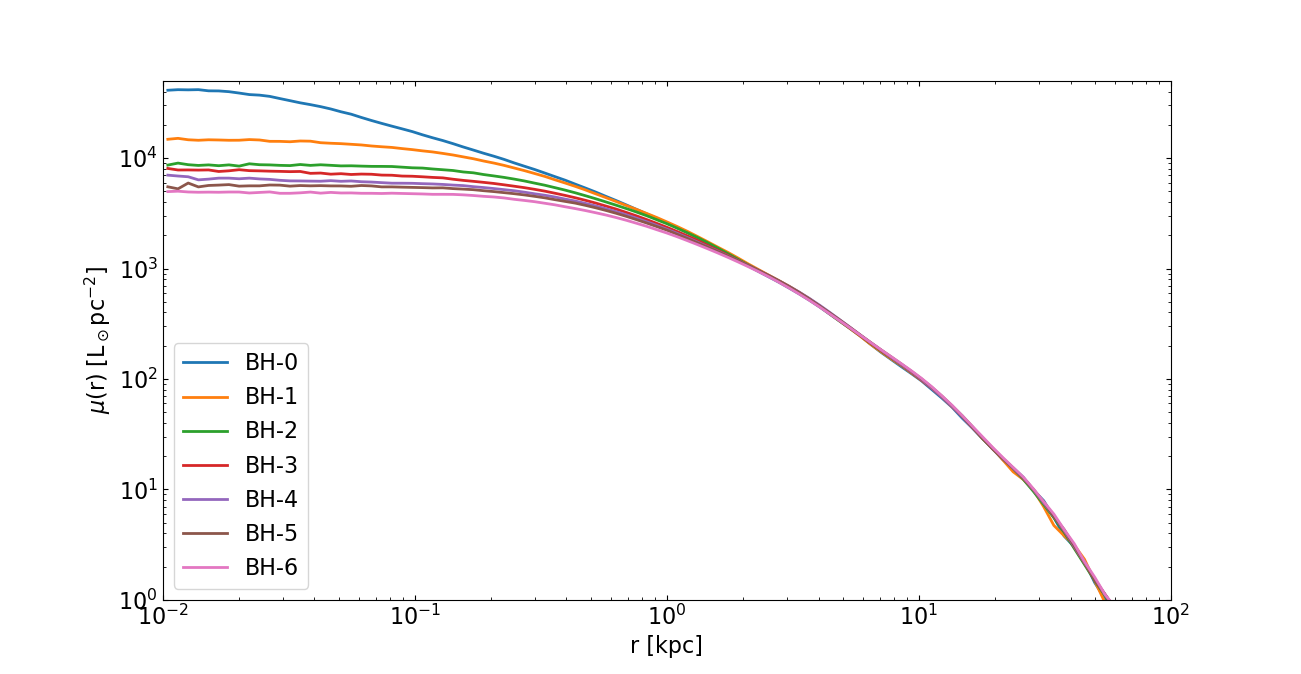
\includegraphics[width=\textwidth]{SurfaceBrightnessProfiles.png}
	\caption{Surface brightness profiles from every simulated merger remnant. These were calculated by dividing the stellar particles in the simulated galaxy remnants into 100 radial logarithmic bins, and averaging the surface brightnesses inside these bins through 100 random viewing angles. The luminosity of the particles was estimated by assuming a constant mass-to-light ratio of $M/L = 4$.}
	\label{figure:surface_brightness}
\end{figure}

The lack of light in the surface brightness profiles reveals the presence of cores; however, determining the precise sizes of the cores requires us to find the exact locations where the deviations from the Sérsic fit begin. This can be done by fitting the derived brightness profile with a model that is a combination of two power laws: a shallow inner power-law, and a steeper outer power-law. The radius at which the outer power-law changes into the inner power-law (and vice-versa) is called the break radius ($r_b$), and can be defined as the radius of the core. 

There are two commonly used options for modelling the surface brightness profiles. The first one is the core-Sérsic profile \citep{Graham2003}, which can be expressed using the following equation:
\begin{equation}
\mu(r) = \mu' \left[ 1 + \left( \frac{r_b}{r} \right)^\alpha \right]^{\gamma / \alpha} \exp \left\lbrace -b_n \left[ \left( r^\alpha + r_b^\alpha \right) / r_e^\alpha \right]^{1/(\alpha n)} \right\rbrace, \label{eq:core-sersic}
\end{equation}
where $r_b$ is the break radius, $\gamma$ is the logarithmic slope of the inner power-law, $\alpha$ controls the sharpness of the transition between the two power-laws, $r_e$ and $n$ are the effective half-mass radius and the Sérsic index of the outer power-law respectively, and the normalization factor $\mu'$ is defined by:
\begin{equation}
\mu' = \mu_b 2^{-\gamma/\alpha} \exp \left[ b_n \left( 2^{(1/\alpha)} r_b/r_e \right)^{1/n} \right], 
\label{eq:mu_dot}
\end{equation}
where $\mu_b$ is the surface brightness at the break radius. 

The second option is to use the so called Nuker profile \citep{Lauer1995}:
\begin{equation}
\mu(r) = 2^{(\beta - \gamma) / \alpha} \mu_b \left( \frac{r_b}{r} \right)^\gamma \left[ 1 + \left( \frac{r}{r_b} \right)^\alpha \right]^{(\gamma - \beta)/\alpha},
\label{eq:nuker}
\end{equation}
where $r_b$ is once again the break radius, $\mu_b$ is the surface brightness at the break radius, $\beta$ and $\gamma$ are the logarithmic slopes of the power-laws inside and outside of the break radius respectively, and $\alpha$ once again describes the sharpness of the transition between the two slopes.

\begin{figure}[h]
	\centering
	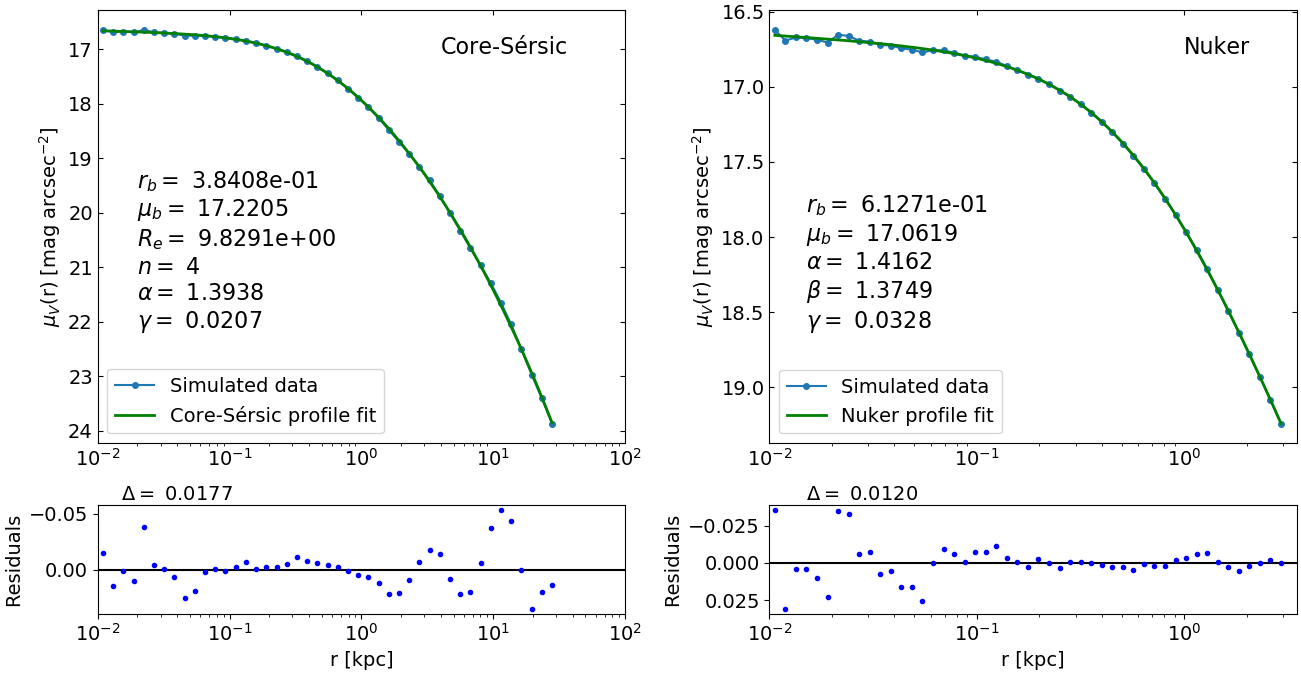
\includegraphics[width=\textwidth]{core_nuker_fits.png}
	\caption{Core-Sérsic and Nuker profile fits of surface brightness profiles calculated from the BH-3 merger remnant (left and right figures respectively). The best fit parameters are shown on the figures and are in the same units as the axes (i.e. $r_b$ and $R_e$ in kilo-parsecs, and $\mu_b$ in V-band magnitudes per arc-second squared). The relative residuals of the fits are plotted under their respective figures. The delta describes the root-mean-square of the residuals.}
	\label{figure:core_nuker}
\end{figure}

We calculate the core radii of the merger remnants by using the "Levenberg-Marquardt" fitting algorithm to fit both the core-Sérsic model and the Nuker model to the remnants' surface brightness profiles. For the most part, the initial guesses for the fitting parameters' values in the fitting algorithm, were determined through trial-and-error, as well as knowledge of their likely order of magnitude. This was not the case for the Sérsic-index ($n$) of the core-Sérsic profile however. In order to reduce degeneracy between the fitting parameters, $n$ was fixed to $n=4$ for all core-Sérsic profile fits.

Figure \ref{figure:core_nuker} shows a comparison between the core-Sérsic and Nuker profile fits for the BH-3 merger (refer to table \ref{table:properties}), while figures \ref{figure:all_core} and \ref{figure:all_nuker} show these fits for every simulated remnant containing an SMBH binary. The values of the best-fit parameters are shown on the figures. The units of the surface brightness are changed from $L_\odot \; \mathrm{pc^{-2}}$ to $\mathrm{mag \; arcsec^{-2}}$ (where $\mathrm{mag}$ is the magnitude in the V-band) using the common conversion formula:
\begin{equation}
\mu = M_\odot + 21.572 - 2.5 \log(I), 
\end{equation}
where $M_\odot$ is the absolute magnitude of the Sun in a specific spectral band (in our case the V-band magnitude of $4.83$ is used), and $I$ is the surface brightness in $L_\odot \mathrm{pc^{-2}}$.

The root-mean-square of the fits' residuals are comparable to the values seen in profile fits of observed surface brightness profiles: $\Delta \approx 0.02 \; \mathrm{mag \; arcsec^{-2}}$ \citep{Dullo2012}. Although, while the RMS of the residuals show that the fits describe the surface brightness profiles rather well, most of the fits have large residual scatter near the centre of the merger remnant. This is especially noticeable in the Nuker fits, since in order to get sensible values for the fitting parameters, the fitting range needs to be concentrated in the galactic centre (in our analysis, the fitting range used for the Nuker profile was: $\sim 0.04 - 3 \; \mathrm{kpc}$, which is an order of magnitude lower compared to the range used for the core-Sérsic fit: $\sim 0.04 - 60 \; \mathrm{kpc}$). 

The larger central residual scatter is most likely not indicative of any kind of physical structure in the merger remnant cores; but simply a result of the logarithmic spacing of the bins in the surface brightness profiles. The bins near the centre inherently contain less particles than the outer bins. When calculating the 100 projected surface brightness profiles from random viewing angles, this causes the variations in binned luminosities to be larger in the central bins, resulting in a final averaged profile that contains small jumps as well as small dips in its central luminosity. These arbitrary inconsistencies naturally cause the residuals of the fits to be scattered in a random way near the centre of the simulated galaxy. Unfortunately, remedying this problem by using bins that have a constant number of particles did not yield satisfactory results, due to the total number of particles being extremely small near the centre.

Interestingly, all of the core-Sérsic fits show a peak in the size of the residuals at around $\sim 10 \; \mathrm{kpc}$. Once again, this residual property is probably just a small anomaly in the simulations and not indicative of any physical structure that could be found in actual merger remnants. However, the fact that this residual anomaly appears in the surface brightness profile of every simulation, indicates that; even though the masses of the SMBHs in the merger progenitors have a large effect on the central regions of the merger remnant, the outer regions are left relatively unaffected. In fact, the central SMBH binary only affects the outer regions of the merger remnant through stellar particles that have been ejected from the galactic centre. 

All of the significant residual variations between the profile fits of the simulated merger remnant galaxies are concentrated near their respective centres. This implies that the results of the different simulations vary significantly from each other only due to the formation of a central SMBH binary, since the similar shapes of the outer regions of the residual plots can be explained through the limited range of the binaries' gravitational spheres-of-influence (SOI). The sizes of the SMBH binaries' SOI can be seen in table \ref{table:s-o-i}. They were calculated by: finding the radius of a sphere (centred at the c.o.m. of the host galaxy) that contains the amount of stellar mass equivalent to the mass of the SMBH binary. The sizes of the projected radii were determined through a similar relation to the one described in equation \ref{eq:projection_approximation}.


\begin{table}
	\begin{center}
		\begin{tabular}{| c | c |}
		\hline
		Simulation & $r_\mathrm{SOI}$ $\mathrm{[kpc]}$ \\
		\hline
		BH-1 merger & 0.143 \\
		BH-2 merger & 0.256 \\
		BH-3 merger & 0.394 \\
		BH-4 merger & 0.515 \\
		BH-5 merger & 0.620 \\
		BH-6 merger & 0.757 \\
		\hline
		\end{tabular}
	\end{center}
	\caption{Estimations of the projected radii of the spheres-of-influence ($r_\mathrm{SOI}$) for every SMBH binary. They were calculated by finding the radius of, a sphere that contains the amount of stellar mass equivalent to the mass of the binary, inside the binary's host merger remnant. The 2D projections of the radii were determined by using a relation similar to the one described in equation \ref{eq:projection_approximation}.}
	\label{table:s-o-i}
\end{table}

\begin{figure}
	\centering
	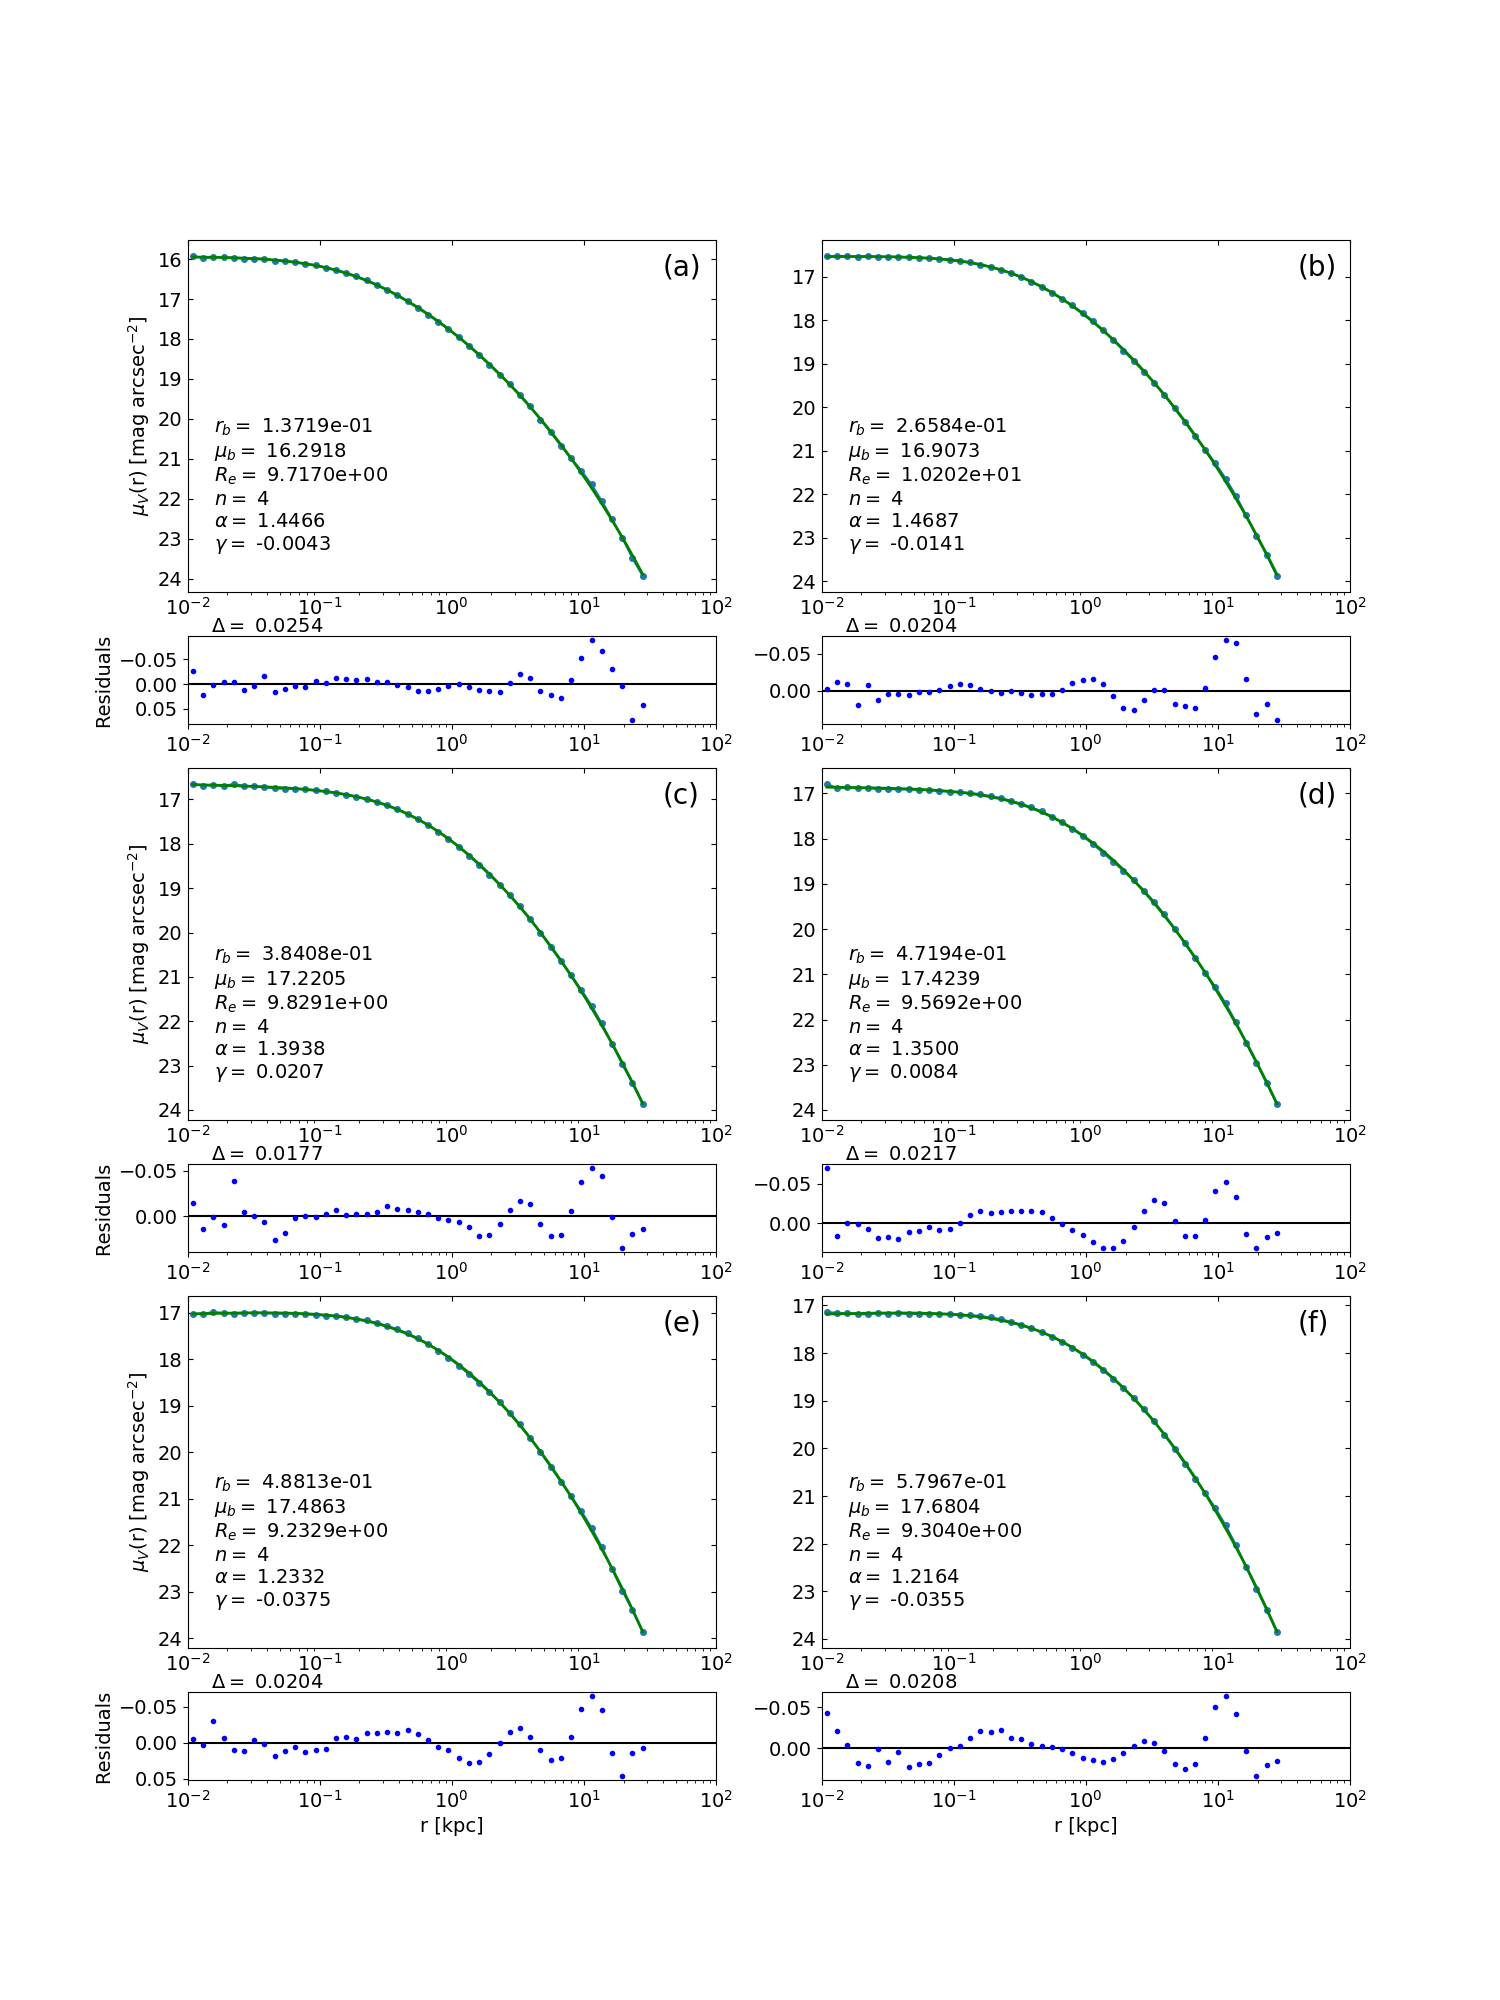
\includegraphics[width=\textwidth]{all_core_profiles.png}
	\caption{Core-Sérsic profile fits of the surface brightness data calculated from all of the individual simulated merger remnants with progenitors containing central supermassive black holes. The letters (a)-(f) denote the different snapshots ((a): BH-1 merger, (b): BH-2 merger, (c): BH-3 merger, (d): BH-4 merger, (e): BH-5 merger, (f): BH-6 merger).}
	\label{figure:all_core}
\end{figure}

\begin{figure}
	\centering
	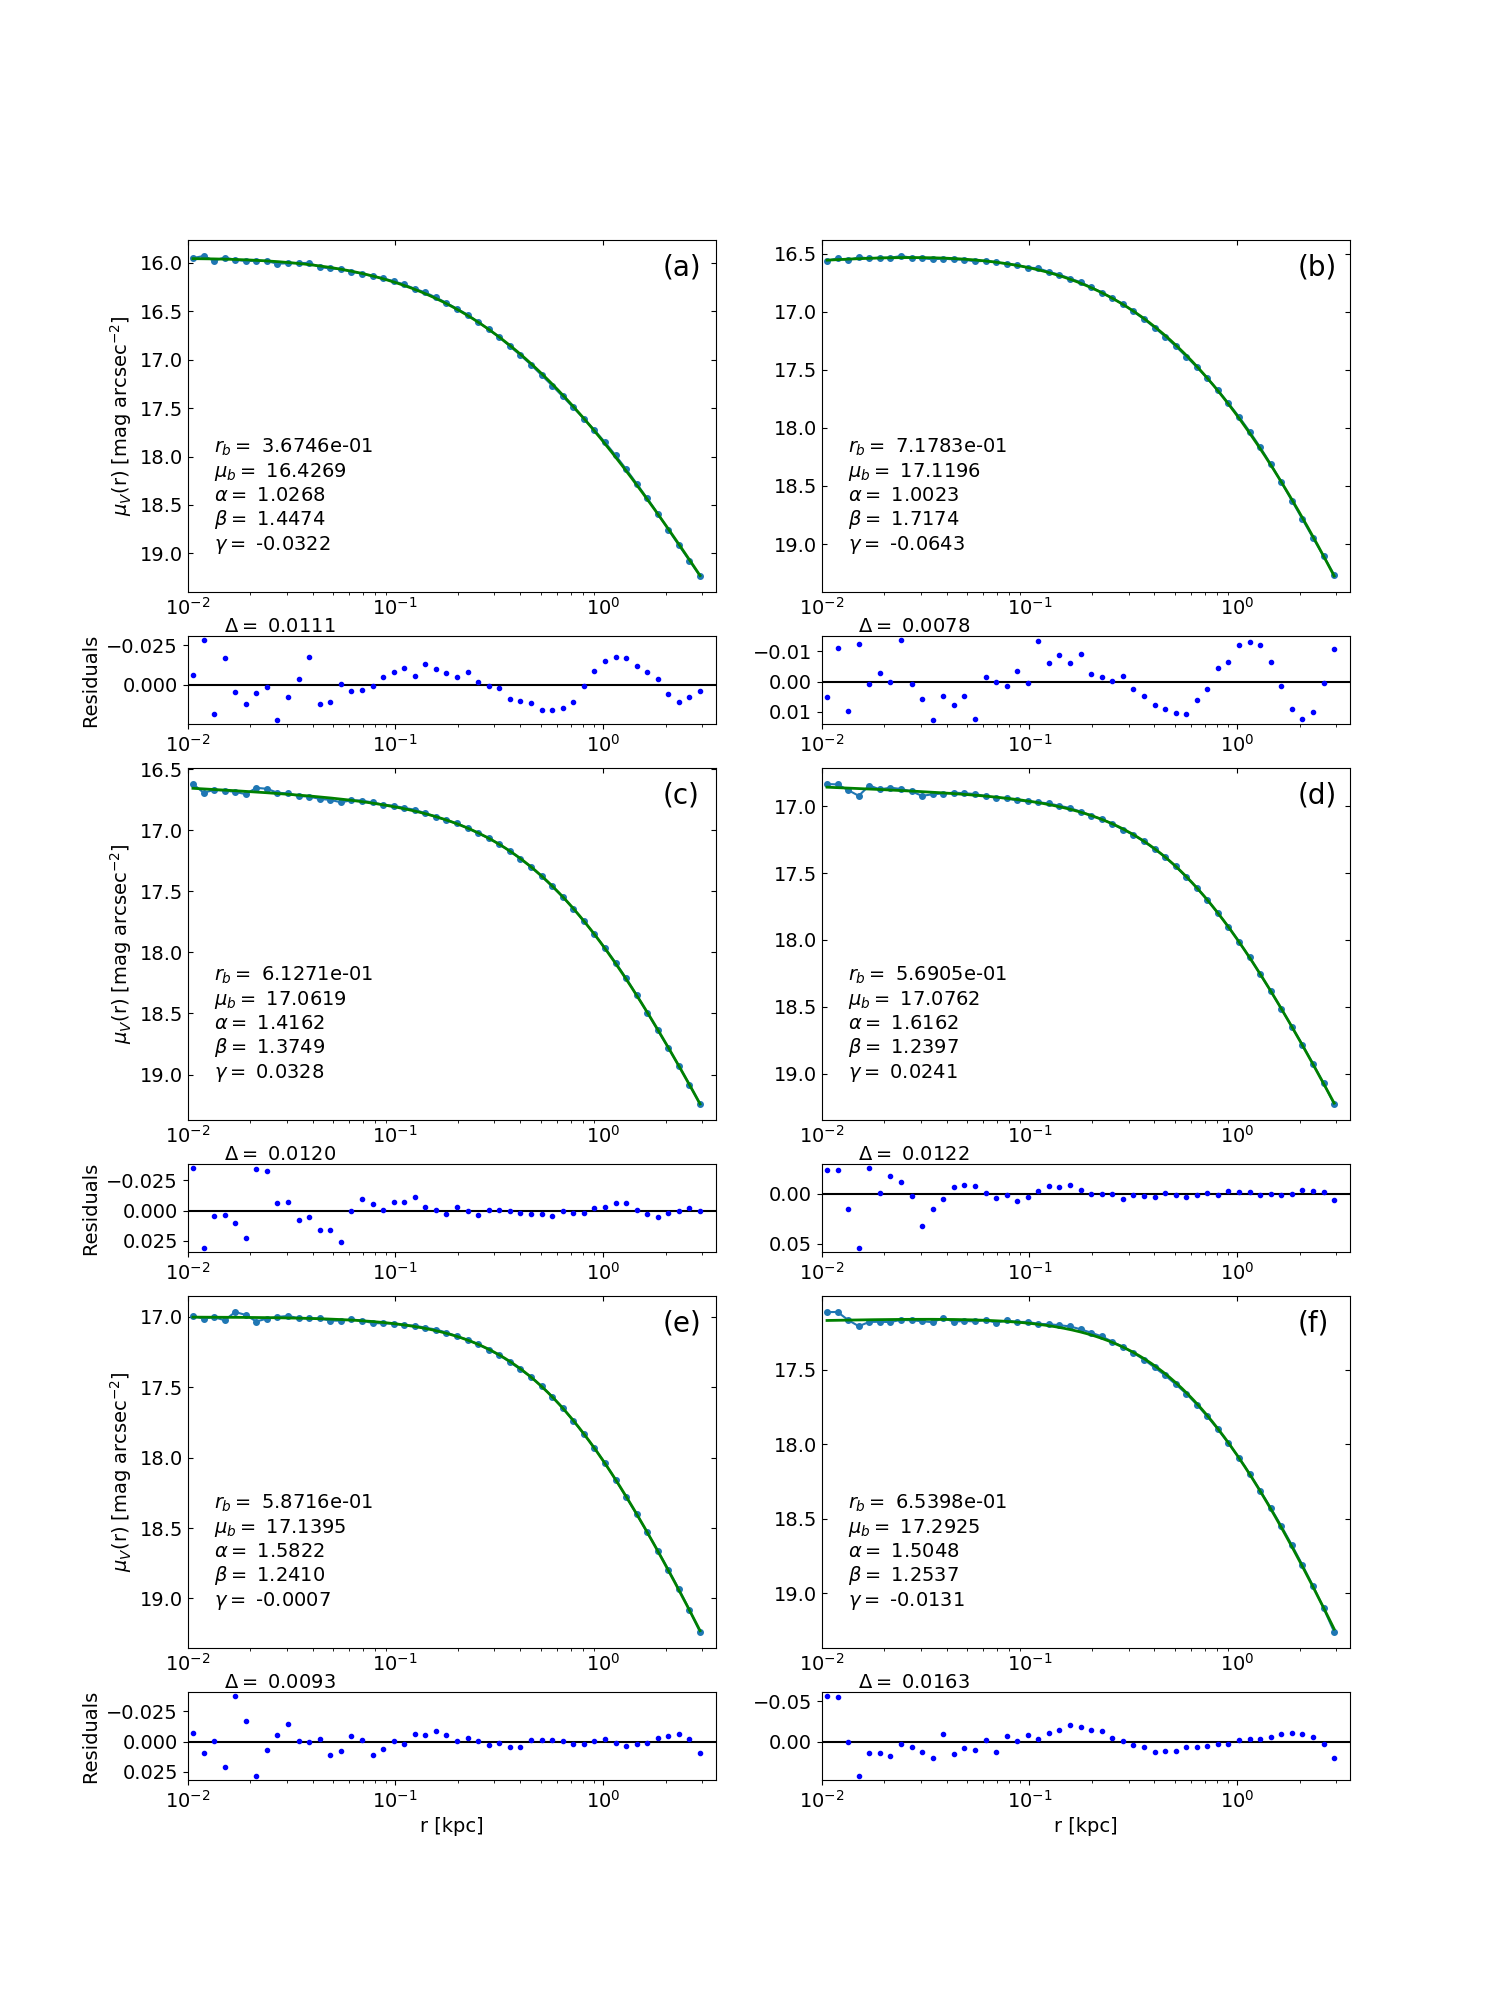
\includegraphics[width=\textwidth]{all_nuker_profiles.png}
	\caption{Nuker profile fits of the surface brightness data calculated from all of the individual simulated merger remnants with progenitors containing central supermassive black holes. The letters (a)-(f) denote the different merger remnants ((a): BH-1 merger, (b): BH-2 merger, (c): BH-3 merger, (d): BH-4 merger, (e): BH-5 merger, (f): BH-6 merger).}
	\label{figure:all_nuker}
\end{figure}

Figures \ref{figure:all_core} and \ref{figure:all_nuker} show that the core radius estimate depends quite strongly on the used fitting model. However, which of the two models is better for estimating the size of the core is still a matter of debate \citep{Lauer2007, Dullo2012}. While the RMS of the relative residuals seems to be consistently (although just marginally) smaller for the Nuker model (compare figures \ref{figure:all_core} and \ref{figure:all_nuker}), one also has to take into account that, in the Nuker model, the best-fit value for $r_b$ is strongly dependent on the fitting range \citep{Graham2003}. Furthermore, as stated by \cite{Rantala2018}, in order to get sensible values for all of the model parameters (e.g. $\alpha$, for which $\alpha \lesssim 1$ might even prevent the model from describing the profile as a combination of two power-laws), the fitting range of the Nuker model has to be narrowed down closer to the galactic centre. This, when combined with the parameters' high dependence on the fitting range, shows that the core radius estimations of the Nuker model can be inconsistent.

In addition to the model fitting methods, one could also estimate the size of the core by calculating the so-called "cusp radius" $r_\gamma$. The cusp radius is the distance from the centre of the galaxy, at which the logarithmic slope of the surface brightness profile equals $\gamma' = -1/2$ \citep{Carollo1997, Lauer2007Cusp}. This distance provides an estimate for the location where the inner power-law of the profile changes into the outer power-law, and thus $r_\gamma$ can be equated to the core radius. 

We calculate $r_\gamma$ for all of the merger remnants with central SMBH binaries (BH-1 - BH-6 mergers) by calculating the gradient of the surface brightness profiles, and then using a function minimization algorithm \citep{NelderMead} to minimize the difference $\big| \frac{d\mu(r)}{dr} - \left( - \frac{1}{2} \right) \big|$. This allows us to find the radius, at which the gradient gets the value $-1/2$. 

\begin{figure}[h]
	\centering
	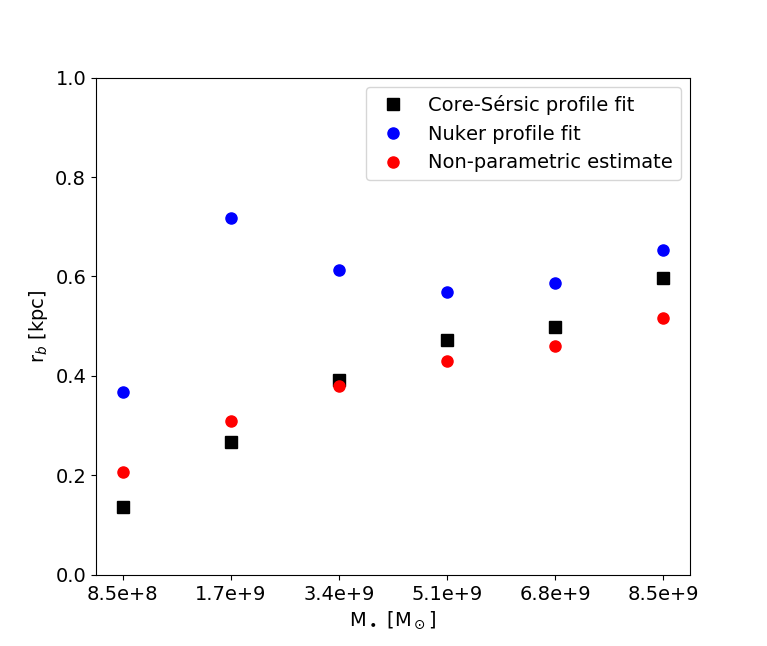
\includegraphics[width=\textwidth]{rb_mass_relation.png}
	\caption{Comparison of the different core radius estimates of the merger remnants. These estimates were derived through three different methods: Core-Sérsic profile fitting (black squares), Nuker profile fitting (blue circles) and  finding the "cusp radius" (red circles). The x-axis shows the masses of the central SMBH binaries in the merger remnants.}
	\label{figure:radii_comparison}
\end{figure}

Figure \ref{figure:radii_comparison} compares the core radius estimates from each of the three methods for every simulated merger remnant. The break radii from the Nuker fits are consistently larger than the other core radius estimates. They also have, in general, the largest deviations from the other core radii, and even contain two values that seem to break the trend of the core radius growing with the central SMBH binary mass (these being the break radii for the BH-2 and BH-3 mergers). Similar larger than expected Nuker core radii can be seen in the analysis of the simulations by \cite{Rantala2018}. Similarly to figure \ref{figure:radii_comparison}, the difference in their Nuker break radii and the other core radius estimates for the two mergers with the smallest and third smallest central SMBH binaries, are significantly larger than for the other mergers. The fact that these large deviations are present in both our analysis and the analysis by \cite{Rantala2018}, further implies that, due to its high dependence on the fitting range, the Nuker model can provide inconsistent values for the break radius. However, when excluding these few Nuker break radii, a clear trend of the size of the core growing with the merger progenitors' central SMBH masses can be seen.

The fact that the size of the core is dependent on the mass of the central SMBH binary is clear evidence towards the cores being formed through a scouring process by the binary black holes. Binaries with larger masses have larger gravitational spheres-of-influence (table \ref{table:s-o-i}), which naturally leads to the ejection of stellar particles that orbit farther away from the galactic centre (the larger SMBH binary mass also causes the stellar material to be ejected at a larger velocity). 

This positive correlation between the core size and the SMBH binary mass has also been identified in independent measurements of the break radius and the central SMBH mass in cored galaxies \citep[e.g.][]{deRuiter2005, Lauer2007Cusp, Thomas2016}. The fact that this effect can be seen, not only in the simulations but also in the observations, makes it clear that merging SMBH binaries are a likely source for the observed cores.

Alongside the size of the core, the surface brightness deficit also becomes larger as the central SMBH binary mass grows, as can clearly be seen in figure \ref{figure:surface_brightness}. This can be explained trough the concept of the loss-cone. \cite{BinneyTremaine} show that only stars with the angular momentum:
\begin{equation}
L \lesssim [G(M_1 + M_2)a]^{1/2},
\end{equation}
where $M_1$ and $M_2$ are the masses of the binary black holes, interact strongly enough with the binary to be ejected from the system (i.e. are inside the loss-cone). As the above equation implies, the upper limit of this condition grows alongside the binary mass. This causes more of the orbiting stellar particles to be located in the strong interaction range; as not only does the loss-cone widen, allowing for the ejection of particles with orbits more parallel to the plane of the binary; but the maximum velocities, at which a stellar particle can interact strongly with the binary, also become larger. Thus, a larger SMBH binary mass naturally results in the ejection of a larger number of stellar particles, which then leads to the growth of the central surface brightness deficit.  

\section{Velocity Anisotropy}

%\begin{figure}[h]
%	\centering
%	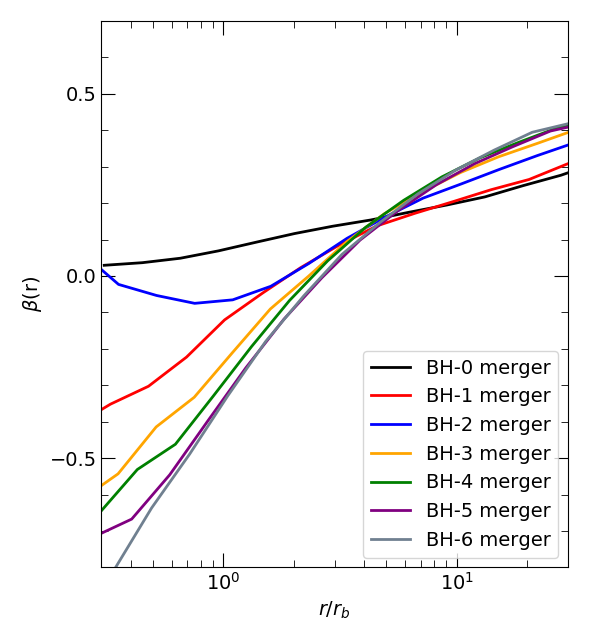
\includegraphics[width=0.9\textwidth]{beta.png}
%	\caption{Velocity anisotropy (beta) profiles of the simulated merger remnants with central black holes.}
%\end{figure}

Another method of studying whether a galaxy has formed a core through core scouring by binary black holes, is to study the velocity anisotropy profile defined in \cite{BinneyTremaine} as:
\begin{equation}
\beta(r) = 1 - \frac{\sigma_\theta^2 + \sigma_\phi^2}{2\sigma_r^2} = 1 - \frac{\sigma_t^2}{\sigma_r^2}, \label{eq:beta}
\end{equation}
where $\sigma_\theta$, $\sigma_\phi$ and $\sigma_r$ are one-dimensional velocity dispersions in the spherical coordinates, and $\sigma_t = \sqrt{(\sigma_\theta^2 + \sigma_\phi^2) / 2}$ is the tangential velocity dispersion. This $\beta$-parameter describes the ratio of tangential velocity dispersion in the stellar system to the radial velocity dispersion and, as such, provides information about the nature of the stellar orbits around the black hole binary. A negative value for $\beta$ shows an abundance of tangential orbits, whereas a positive $\beta$ corresponds to an abundance of radial orbits. 

Figure \ref{figure:beta_no_rb} shows $\beta$-profiles calculated from all of the final merger remnant snapshots using equation \ref{eq:beta}. In order to get the velocity dispersions, the stellar particles of the remnants were first divided into logarithmic bins, and their velocities were changed from a Cartesian to a spherical coordinate system. Next, the root-mean-squares, which correspond to the velocity dispersions, of the different spherical velocity components were calculated for each bin separately, resulting in a $\beta$-value for every bin. Plotting these values gives us the aforementioned profiles in figure \ref{figure:beta_no_rb}. 

\begin{figure}[h]
	\centering
	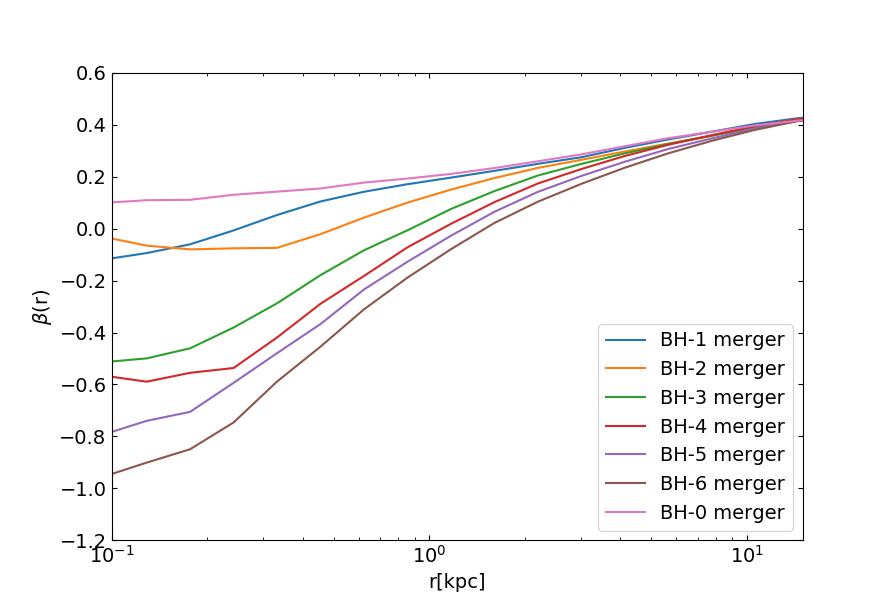
\includegraphics[width=0.9\textwidth]{beta_no_rb.png}
	\caption{Velocity anisotropy (beta) profiles for every simulated merger remnant. The profiles are calculated from the velocity dispersions in radial logarithmic bins, using equation \ref{eq:beta}. Going from the outer regions to the central regions of the merger remnants, the profiles of the remnants with SMBH binaries go from being radially dominated to being tangentially dominated.}
	\label{figure:beta_no_rb}
\end{figure}

According to the $\beta$-profiles, the outer areas of the remnants are dominated by radial orbits (positive $\beta$), while the majority of orbits near the centre are tangential (negative $\beta$). As the initial merger progenitors used in the simulations contained isotropic $\beta$-profiles ($\beta = 0$), an area with negative $\beta$ in the merger remnant would imply that the stars on radial orbits have been lost from the system. It has been shown that hardening black hole binaries can eject stars on highly radial orbits from the galactic core, which results in the central region becoming dominated by mostly tangential orbits (and thus a negative $\beta$). The ejected stars can then, in turn, cause the outer orbits to become more radial \citep{Quinlan1997, Milosavljevic2001, Thomas2014}. 

Figure \ref{figure:beta_no_rb} clearly shows that the presence of an SMBH binary has an effect on the shape of the $\beta$-profiles. Not only is the slope of the profile steeper for merger remnants which contain a more massive central SMBH binary, but the only merger with a profile that is completely dominated by radial velocity dispersion, is the one without a central SMBH binary (the BH-0 merger). 

The shapes of the profiles also make sense in the context of ejection of stellar particles by hardening black hole binaries. The larger the mass of the SMBH binary is, the larger its gravitational sphere-of-influence, which results in more of the radially orbiting stellar particles being ejected.

\begin{figure}
	\centering
	\begin{subfigure}[b]{0.39\textwidth}
		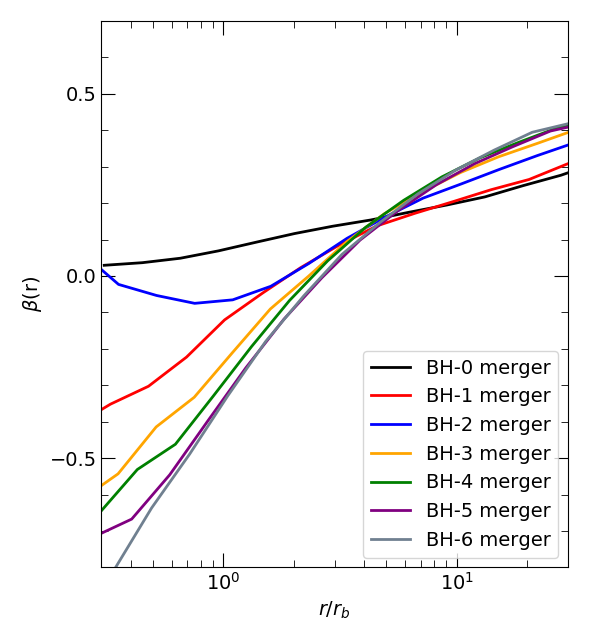
\includegraphics[width=\textwidth]{beta.png}	
		\caption{Simulated merger remnants}
	\end{subfigure}
	\begin{subfigure}[b]{0.60\textwidth}
		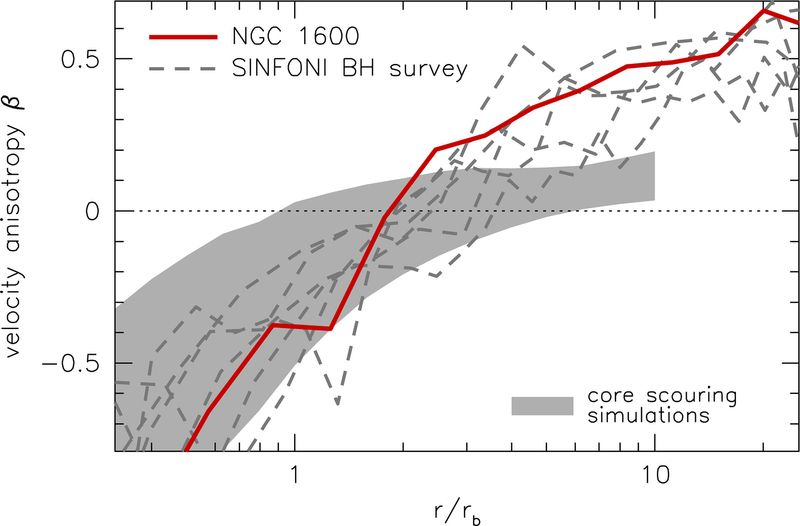
\includegraphics[width=\textwidth]{thomas2016.jpg}
		\caption{NGC 1600}
	\end{subfigure}
	\caption{(a): The $\beta$-profiles of the simulated merger remnants as a function of distance from the centre, scaled by their respective break radius. For the merger remnant without a core (BH-0), the value used for the break radius is $r_b = 1 \; \mathrm{kpc}$. The profile for the BH-2 merger shows an increase in the value of $\beta$ near the centre of the merger remnant, which is simply the same increase seen in figure \ref{figure:beta_no_rb} amplified by the break radius scaling. (b): $\beta$-profile of NGC 1600, alongside profiles of galaxies from the SINFONI black hole survey \citep{Saglia2016} and the range of possible anisotropies found in N-body simulations of the core scouring mechanism \citep{Thomas2016}.}
	\label{figure:beta_NGC1600_Simul}
\end{figure}

Figure \ref{figure:beta_NGC1600_Simul} shows, both the observed $\beta$-profile of NGC 1600 and the profiles from our simulated merger remnants. The profiles in the figure are scaled by the core radius of the respective galaxy. Even by eye, it can clearly be seen that the $\beta$-profiles from both the simulations and the observations of NGC 1600 are similar to each other (not counting the anomalous profile for the BH-2 merger). However, looking closely at the values on the axes of the plots, the observed profile of NGC 1600 seems to be somewhat steeper when compared to any of the simulated ones.

%According to \cite{Rantala2018} it is likely that, the larger steepness of the profile seen in NGC 1600 is due the simulations only comprising a single generation of completely isotropic ($\beta = 0$) mergers. Most observed cored galaxies, including NGC 1600, are most likely the result of multiple generations of mergers. The progenitors of the observed major merger remnant galaxy would thus have already had tangentially biased $\beta$-profiles, leading to a remnant with an even steeper profile.

According to \cite{Rantala2018}, the kinematics being more tangential close to the core in NGC 1600 than in the simulations, could be caused by further adiabatic growth of the merged central SMBH's mass. \cite{Young1980} shows that black holes that grow adiabatically through, for example accretion of gas, can cause the surrounding stellar orbits to become more tangential. If the time scale of the mass growth is smaller than the relaxation time scale of the galaxy while also being larger than the dynamical time scale of the stellar system, the growth can be considered adiabatic. This results in the conservation of the angular momentum and the radial action of the stellar orbits (radial action being one of the momenta in the canonical Hamiltonian coordinates called \textit{angle-action variables} \citep[e.g.][]{BinneyTremaine}, which, due to the now higher gravitational potential induced by the central black hole, causes the orbits to become more circular. Although this effect is not strong enough to account for the entire shape of the $\beta$-profile \citep{Thomas2016}, it could certainly be a reason for the more tangentially dominated core regions seen in the observations.

As for the outer region of the $\beta$-profile of NGC 1600, it is possible, that the reason why it is more radially dominated than any of the outer parts in the simulated merger remnants, is due to the lack of minor-mergers in the simulations \citep{Rantala2018}. These minor-mergers would deposit all of their mass in the outer regions of the galaxy, and would thus disrupt only the outer stellar orbits, making some of the more tangential of these orbits more radial. Furthermore, they would not contribute to the destruction of radial orbits near the centre of the galaxy, as the smaller progenitor galaxy would not contain a central SMBH.

\section{Line-of-Sight Kinematics}

\subsection{2D Kinematic Maps}

In order to make sure that the KETJU simulations produce results which are in agreement with observations, I  also analyse the line-of-sight (LOS) kinematics of the simulated merger remnants. The analysis is focused on four different LOS velocity distribution parameters: the average LOS velocity $V_\mathrm{avg}$, the velocity dispersion $\sigma$, and the $h_3$ and $h_4$ parameters which correspond to the skewness and the kurtosis of the distribution respectively. The distribution from which these properties are calculated is defined as the following modified Gaussian function \citep{VanDerMarel1993, Bender1994}:
\begin{equation}
f(v) = I_0 e^{-\gamma^2/2}(1 + h_3 H_3(y) + h_4 H_4(y)), 
\end{equation} 
where $I_0$ is a normalization constant, $\gamma$ is the central slope of the particle density profile, $y = (v - V_\mathrm{avg})/\sigma$, and $H_3$ and $H_4$ are the third and fourth order Hermite polynomials respectively:
\begin{eqnarray}
H_3(y) = \left(2\sqrt{2}y^3 - 3\sqrt{2}y\right) / \sqrt{6}, \\
H_4(y) = \left(4y^4 - 12y^2 + 3 \right) / \sqrt{24}.
\end{eqnarray}

The above properties are calculated using a Python-script (Matteo Frigo, internal communication), which makes use of the Voronoi tessellation algorithm by \citep{Cappellari2003} in order to provide binned statistics of the LOS velocities. First, when using the script, the "line-of-sight" is defined as the intermediate axis of the merger remnant, after which the remnant is oriented accordingly using the inertia tensor. The 2D line-of-sight projection of the remnant is then divided into "spaxels" (or simply bins) using the aforementioned Voronoi tessellation algorithm. The shape and size of the spaxels are determined so that each one contains the same signal-to-noise ratio, which in our simulated case is defined as the number of stellar particles. The LOS-velocities inside the spaxels are then made into a histogram, into which the modified Gaussian function described in equation \ref{eq:mod_gaussian} is fitted. This gives the values of the LOS-velocity distribution parameters: $V_\mathrm{avg}$, $\sigma$, $h_3$ and $h_4$ for the spaxel in question. Finally, the values of the spaxels can be plotted, resulting in 2D voronoi binned maps of all of the four parameters.

Figure \ref{figure:IFU-maps} shows the voronoi binned 2D maps of the four LOS velocity distribution parameters for the simulated BH-0 merger (no central SMBH) and the BH-6 merger (largest central SMBH), as well as for two observed galaxies NGC 3414 and NGC 4111. The contours, which are added to help visualise the shape of the galaxy, denote flux isophotes of the merger remnants, and have a spacing of one magnitude. Similar maps for the rest of the simulated merger remnants can be seen in figure \ref{figure:rest_of_voronoi}. Figure \ref{figure:rest_of_voronoi} shows the IFU-maps of the four LOS-velocity parameters for the rest of the simulated merger remnants.

The IFU maps in figures \ref{figure:IFU-maps} and \ref{figure:rest_of_voronoi} show that the average LOS velocities of the simulated merger remnants are far from isotropic, with most of the remnants containing central binary SMBHs showcasing counter-rotating central regions also known as "kinematically decoupled cores" (KDC). Some of the simulated remnants (BH-4 - BH-6 mergers) even contain another counter rotating structure inside the KDC \citep{Rantala2019}. These features, alongside the relatively low average LOS-velocities, are often found in galaxies called "slow rotators" \citep{Emsellem2007}. Slow rotator galaxies are early-type galaxies which are assumed to have been formed through gas-poor "dry" mergers \citep{Emsellem2007, Cappellari2007}; processes not unlike the ones simulated in our simulations. As such, the merger remnants being slow rotators is a somewhat expected result.

\begin{figure}
	\centering
	\begin{subfigure}[b]{0.49\textwidth}
		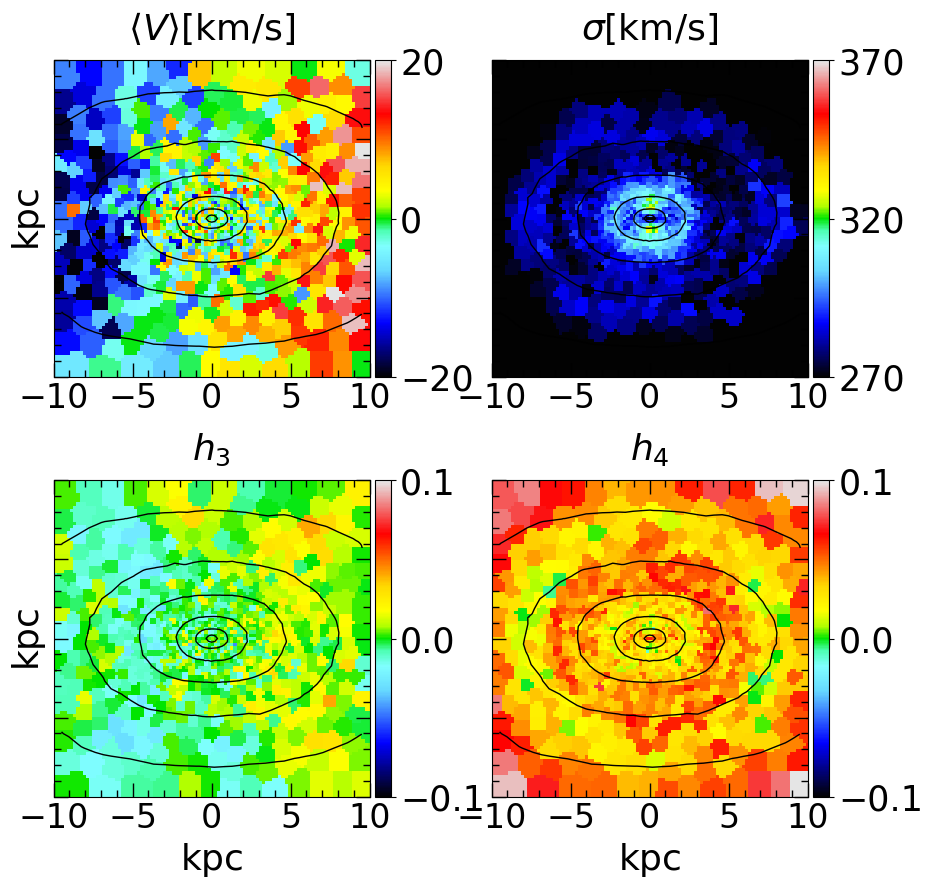
\includegraphics[width=\textwidth]{BH_0.png}
		\caption{BH-0 merger remnant}
	\end{subfigure}
	\begin{subfigure}[b]{0.49\textwidth}
		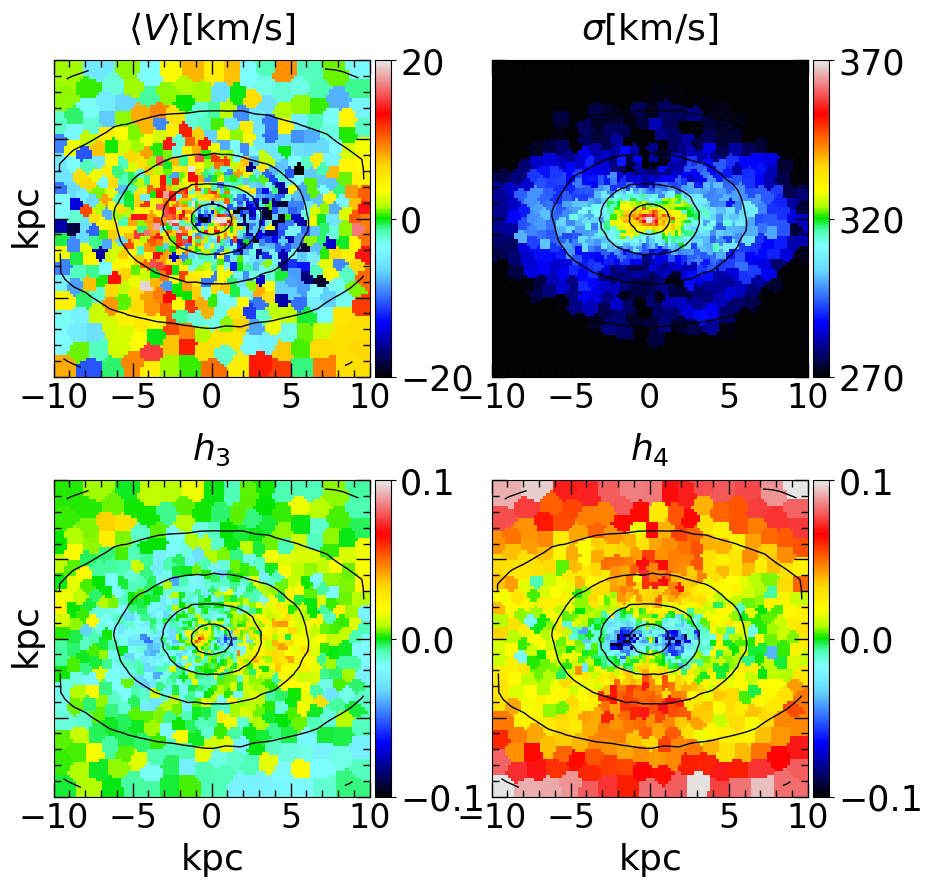
\includegraphics[width=\textwidth]{BH_6.png}
		\caption{BH-6 merger remnant}
	\end{subfigure}
	\begin{subfigure}[b]{0.49\textwidth}
		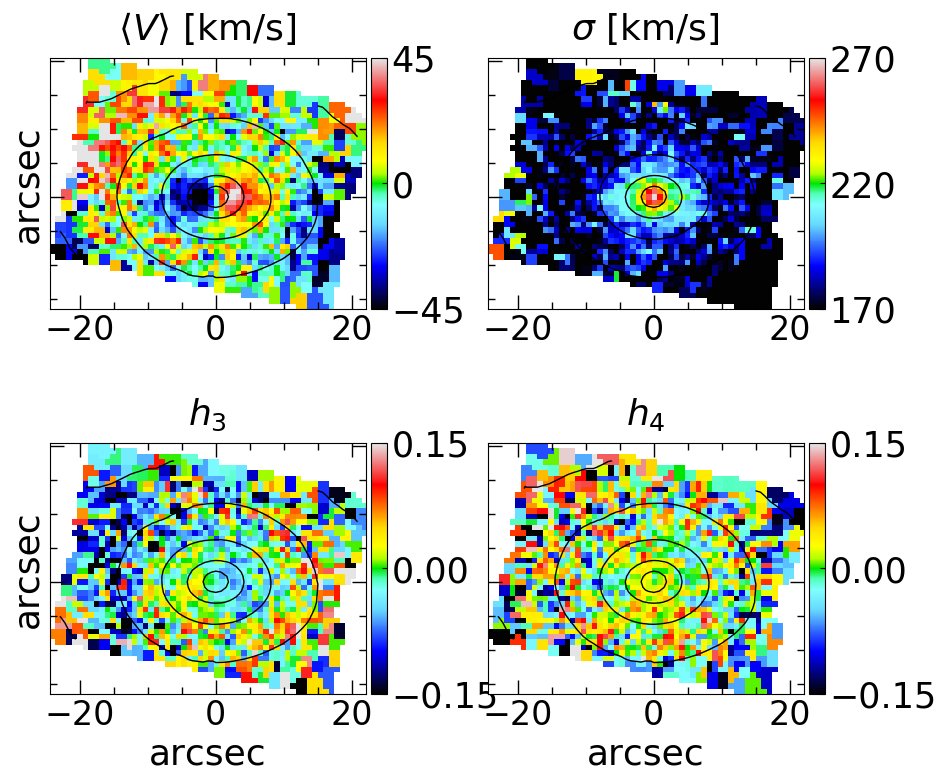
\includegraphics[width=\textwidth]{NGC3414_r6_voronoi.png}
		\caption{NGC 3414}
	\end{subfigure}
	\begin{subfigure}[b]{0.49\textwidth}
		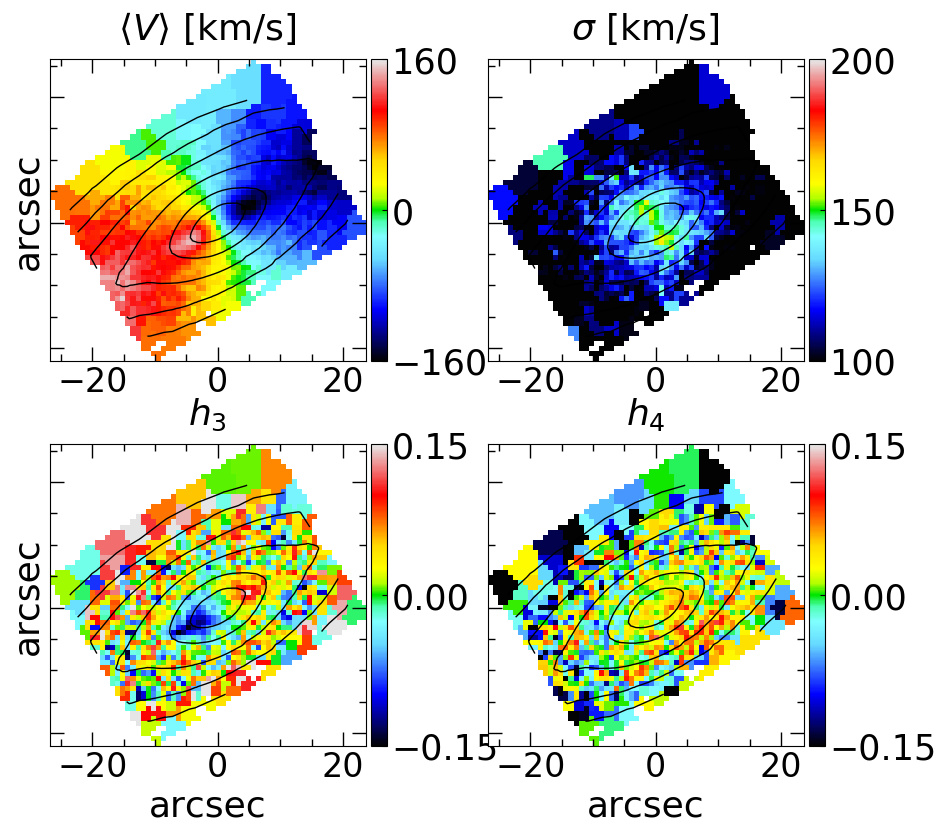
\includegraphics[width=\textwidth]{NGC4111_r1_voronoi.png}
		\caption{NGC 4111}
	\end{subfigure}
	\caption{IFU-maps of average LOS-velocities, velocity dispersion, $h_3$ parameters and $h_4$ parameters from two simulated merger remnants and two observed galaxies. The four maps in figure (a) are from the BH-0 merger, and the four in figure (b) are the BH-6 merger. Figures (c) and (d) show IFU-maps of known slow (NGC 3414) and fast rotator (NGC 4111) galaxies from the $\mathrm{ATLAS^{3D}}$ survey \citep{Emsellem2004, Cappellari2011, Krajnovic2011}.}
	\label{figure:IFU-maps}
\end{figure}

Figures \ref{figure:IFU-maps} and \ref{figure:rest_of_voronoi} also contain IFU-maps of the velocity dispersion in the simulated merger remnants. These maps show a clear connection between the mass of the central SMBH binary and the velocity dispersion at the centre of the galaxy. The presence of an SMBH binary causes the formation of a central velocity dispersion peak in the $\sigma$-distribution, the strength of which correlates positively with the mass of the binary. Furthermore, as the mass of the SMBH binary grows, the size of the area with the highest velocity dispersion in the galaxy also grows. Additionally, the growing binary mass seems to cause the high-$\sigma$ area to get more and more aligned with the major-axis of the galaxy. Most of these effects can easily be identified when comparing the IFU-maps of the different simulated merger remnants from figure \ref{figure:rest_of_voronoi}. The formation of the velocity dispersion peak, which is simply caused by the presence of the SMBH binary, is demonstrated in the IFU-maps of the BH-0 and BH-6 merger remnants in figure \ref{figure:IFU-maps}. The positive correlation between the mass of the central SMBH (or in the case of the simulations: central SMBH binary) and the velocity dispersion of its host galaxy has been observed in a multitude of galaxies with central SMBHs, both cored and non-cored \citep{Ferrarese2000}.

\begin{figure}
	\centering
	\begin{subfigure}[b]{0.49\textwidth}
		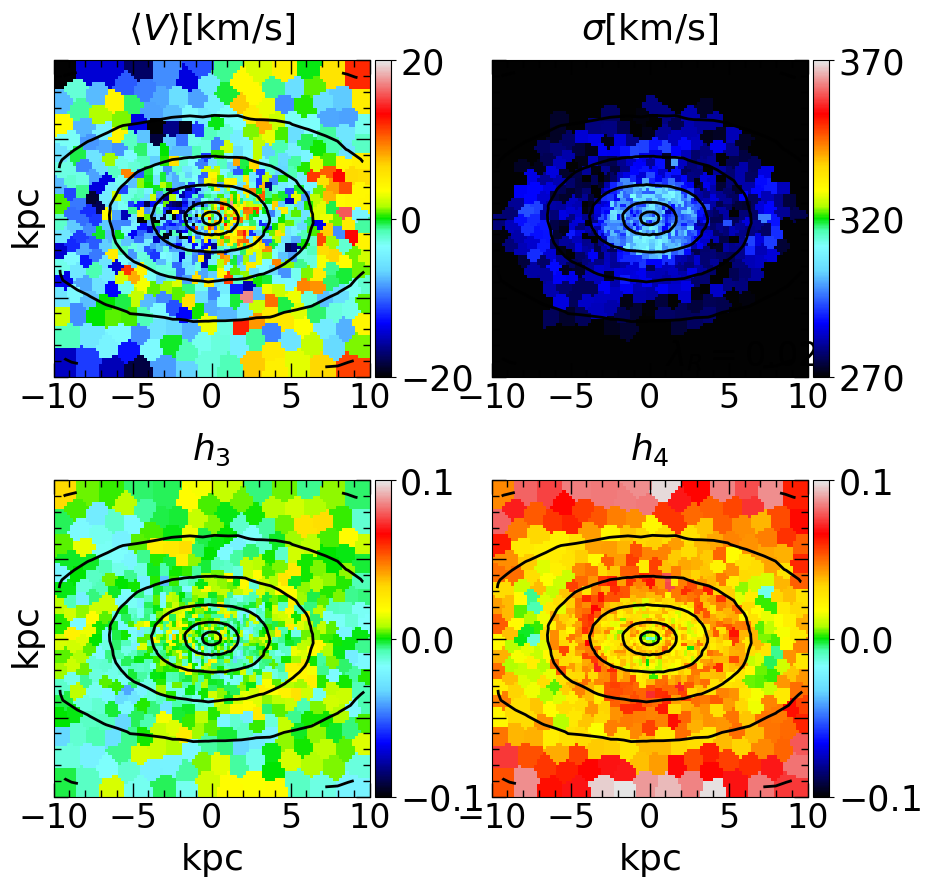
\includegraphics[width=\textwidth]{BH_1.png}
		\caption{BH-1 merger}
	\end{subfigure}
	\begin{subfigure}[b]{0.49\textwidth}
		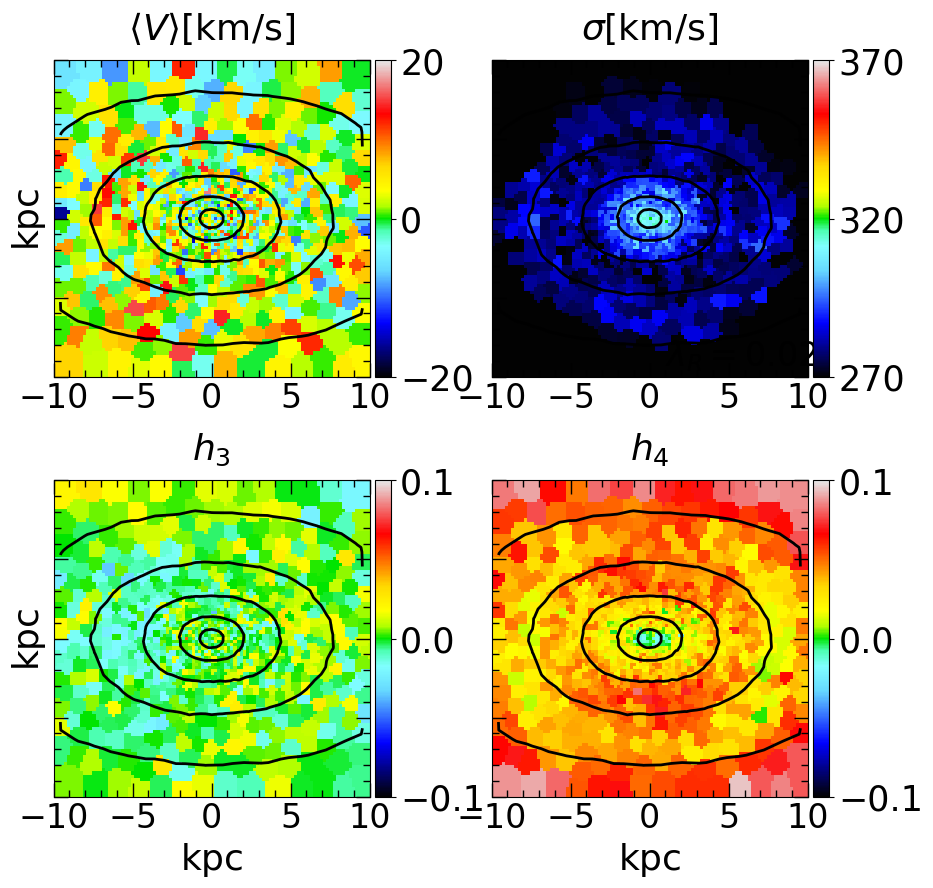
\includegraphics[width=\textwidth]{BH_2.png}
		\caption{BH-2 merger}
	\end{subfigure}
	\begin{subfigure}[b]{0.49\textwidth}
		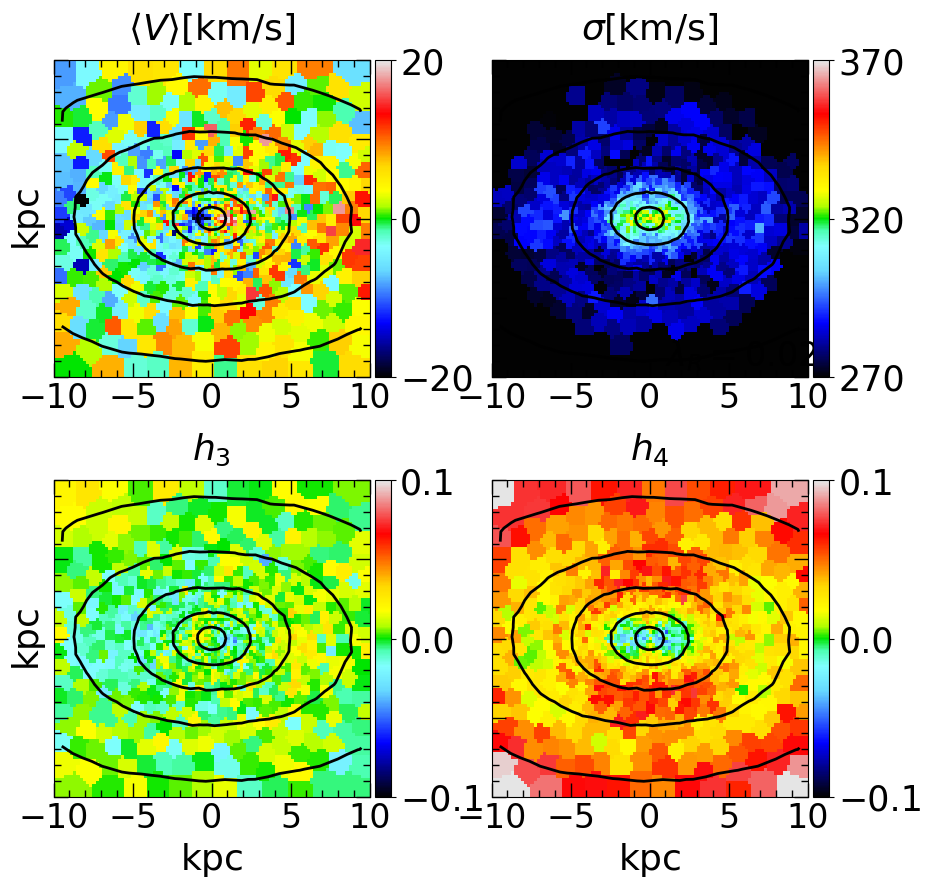
\includegraphics[width=\textwidth]{BH_3.png}
		\caption{BH-3 merger}
	\end{subfigure}
	\begin{subfigure}[b]{0.49\textwidth}
		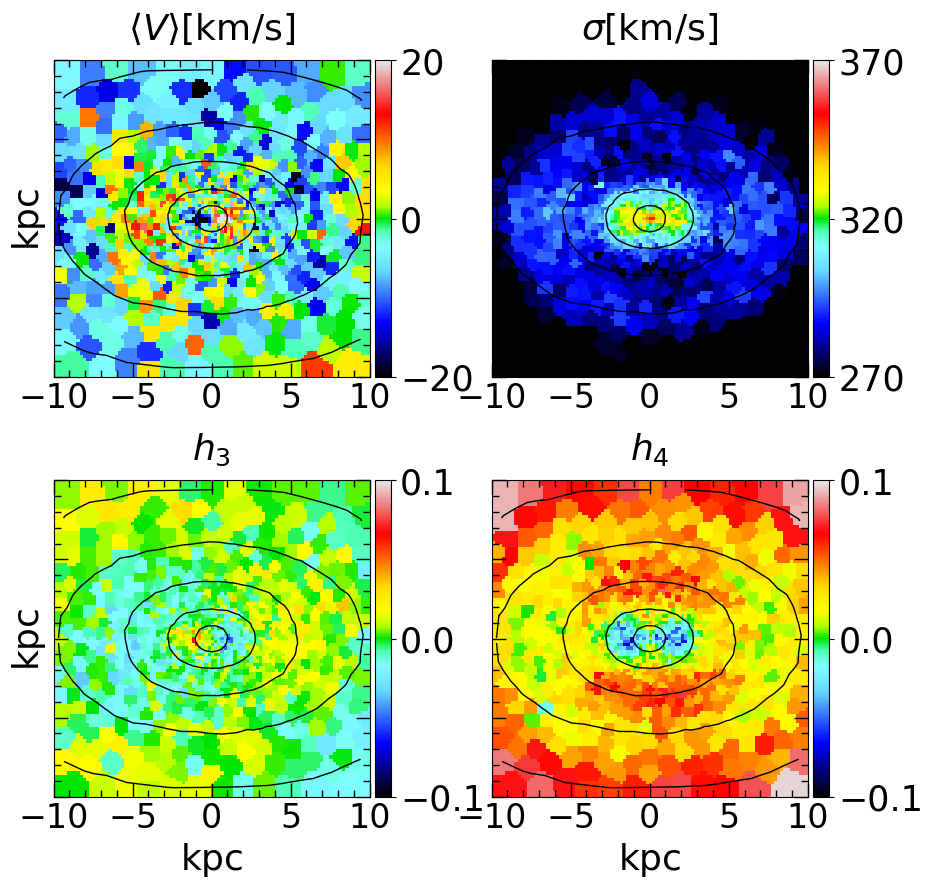
\includegraphics[width=\textwidth]{BH_4.png}
		\caption{BH-4 merger}
	\end{subfigure}
	\begin{subfigure}[b]{0.49\textwidth}
		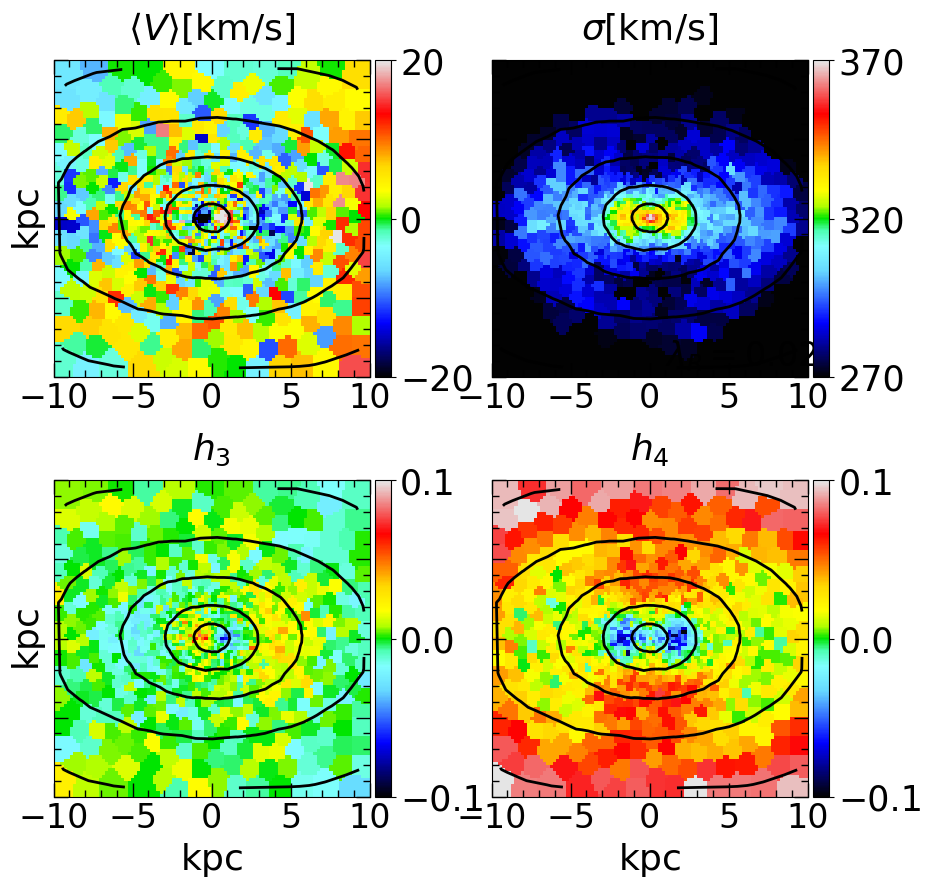
\includegraphics[width=\textwidth]{BH_5.png}
		\caption{BH-5 merger}
	\end{subfigure}
	\caption{IFU-maps of average LOS-velocities, velocity dispersion, $h_3$ parameters and $h_4$ parameters from four simulated merger remnants: BH-1, BH-2, BH-3, BH-4 and BH-5 mergers.}
	\label{figure:rest_of_voronoi}
\end{figure}


 %Furthermore, the velocity dispersion maps also show features found in observed galaxies (figure \ref{figure:IFU-maps}). \textit{Stuff about the features?}

Apart from the BH-0 merger remnant, the $h_3$-parameter values in the IFU-maps of the simulated merger remnants show an anti-correlation with the average LOS-velocity. Indeed, \cite{Krajnovic2011} have found that, while the anti-correlation between the LOS velocities and the $h_3$-parameter is mostly found in fast rotators (see central region of NGC 4111 in figure \ref{figure:IFU-maps}), some galaxies with counter-rotating cores (CRC) also exhibit this behaviour. This anti-correlation can be seen in NGC 3414 from figure \ref{figure:IFU-maps}. Once again, the simulated KETJU results agree with the observations.

The $h_4$-parameter roughly corresponds to the velocity anisotropy parameter $\beta$, where a negative value of $h_4$ identifies areas with a large tangential velocity dispersion, and a positive identifies areas with a more radial velocity dispersion \citep{Gerhard1993, Gerhard1998, Thomas2007}. Comparing the $\beta$-profiles from figure \ref{figure:beta_no_rb} with the $h_4$ IFU-maps from figures \ref{figure:IFU-maps} and \ref{figure:rest_of_voronoi}, this certainly seems to be the case. For the merger remnants with central SMBH binaries, both the $\beta$ and the $h_4$ values are largely positive in the outer regions of the galaxy, while being negative closer to their centres. The $h_4$ map of the BH-0 merger is then positive all around, exactly like its $\beta$-profile. The $h_4$ maps of NGC 3414 and NGC 4111 (figure \ref{figure:IFU-maps}) do not contain any specific structures and seem to be completely isotropic. As the negative $h_4$-areas in the IFU maps of the simulated merger remnants are likely caused by core scouring, and as neither of the observed galaxies are cored galaxies \citep{Lauer2007}; they most likely have not experienced such a process, making the lack of clear structures understandable.

\subsection{The $\lambda_R$-parameter}

Further analysis of the kinematics of the simulated merger remnants can be done by studying the $\lambda_R$ parameter, which describes the angular momentum of a galaxy \citep{Emsellem2007}. More importantly, the parameter allows us to differentiate between the aforementioned slowly rotating galaxies and so-called fast rotators (see figure \ref{figure:IFU-maps}) \citep{Emsellem2007}. The parameter itself is defined in a general form as:
\begin{equation}
\lambda_R \equiv \frac{\langle R |V| \rangle}{\langle R \sqrt{V^2 + \sigma^2} \rangle},
\end{equation}
where $R$ is the projected distance from the galactic centre, $V$ is the line-of-sight velocity, $\sigma$ is the velocity dispersion and $\langle \; \rangle$ denote that the nominator and denominator in the equation are luminosity weighted means. However, as most of the observational kinematic analysis of galaxies is done through binned 2D spectroscopy, and as the IFU-maps made from our simulations are produced the same way as the observed ones, we will be using the following version of the equation:
\begin{equation}
\lambda_R = \frac{\sum^{N_p}_{i=1} F_i R_i |V_i|}{\sum^{N_p}_{i=1} F_i R_i \sqrt{V_i^2 + \sigma^2_i}},
\end{equation}
where $F_i$, $R_i$, $V_i$ and $\sigma_i$ are the flux, projected distance from the galaxy centre, velocity and velocity dispersion of the $i$th bin, and $N_p$ is the number of bins. In the case of our simulations, the $N_p$ bins used are of course the voronoi bins described earlier in this section. 

Determining whether a galaxy is either a fast or a slow rotator using $\lambda_R$, is done by comparing the value that the parameter gets at the galaxy's effective radius, to some pre-defined threshold. The originally used threshold is: $\lambda_{Re} < 0.1$, where $\lambda_{Re}$ is the aforementioned $\lambda_R$ at the effective radius, and where galaxies fulfilling this condition are classified as slow rotators \citep{Emsellem2007}. A revision of the threshold by \cite{Emsellem2011} takes the ellipticity ($\epsilon$) of the galaxy into account, and defines slow rotators as having $\lambda_{R_e} < 0.31 \sqrt{\epsilon}$, which accounts for the increased anisotropy in the kinematics of flatter galaxies. An even further refinement of the slow rotator definition has been proposed by \cite{Cappellari2016}, where slow rotator galaxies are determined using the following two criteria: $\lambda_{R_e} < 0.08 + \epsilon/4$ and $\epsilon < 0.4$. The former criterion of the threshold reduces the risk of misidentifying very round non-regular slow rotators as fast rotators, while the latter makes sure that only sufficiently round galaxies are classified as slow rotators (\citealt{Cappellari2016} argues that "genuine" disk-less slow rotators are all rounder than $\epsilon = 0.4$).

As two of the three aforementioned slow rotator thresholds require us to know the ellipticity of the galaxy I wrote a program in Python that calculates ellipticities of the simulated merger remnants. These ellipticity calculations are done using a method described in \cite{Zemp2011}, which uses the shape tensor:
\begin{equation}
\mathbf{S} = \frac{\int_V \rho(\mathbf{r}) \omega(\mathbf{r}) \mathbf{r} \mathbf{r}^T \; dV }{\int_V \rho{\mathbf{r}} \; dV},
\end{equation}
where $\mathbf{r}$ is position from the galactic centre, $\rho(\mathbf{r})$ is the mass density, $V$ is the volume of an enclosed ellipsoid with the elliptical radius $r_\mathrm{ell}$, and where the weighting function $\omega(\mathbf{r}) = 1$. The eigenvalues of the shape tensor correspond to $a^2/3$, $b^2/3$ and $c^2/3$; where $a$, $b$ and $c$ are the semi-principal axes; and they can be used to calculate the ellipticity as $\epsilon = 1 - b/a$. 

However, simply calculating the shape tensor and getting the correct eigenvalues is not possible, as the elliptical radius $r_\mathrm{ell}$ is defined, in part, by using the axis ratios $a/b$ and $a/c$:
\begin{equation}
r_\mathrm{ell} = \sqrt{x_\mathrm{ell}^2 + \frac{y_\mathrm{ell}^2}{(b/a)^2} + \frac{z_\mathrm{ell}^2}{(c/a)^2}}.
\end{equation}
This means that we have to turn the calculation into an iterative process by starting with $b/a = c/a = 1$ for the initial value of $r_\mathrm{ell}$, and calculating new shape tensor eigenvalues using previously gained axis ratios until the values of the ratios start to converge. 

We calculate $\lambda_{Re}$ and $\epsilon_e$, i.e. the ellipticity at the effective radius (the ellipticity is calculated using $r_\mathrm{ell} = R_e$, and a convergence criterion of a difference smaller than $10^{-3}$ between consequent axis ratios), for every merger simulation snapshot and plot them against each other. We also plot the previously mentioned slow rotator thresholds, as well as observations from the $\mathrm{ATLAS^{3D}}$-survey \citep{Cappellari2011}, in the same figure. The resulting plot can be seen in figure \ref{figure:lambda_epsilon}. 

\begin{figure}[h]
	\centering
	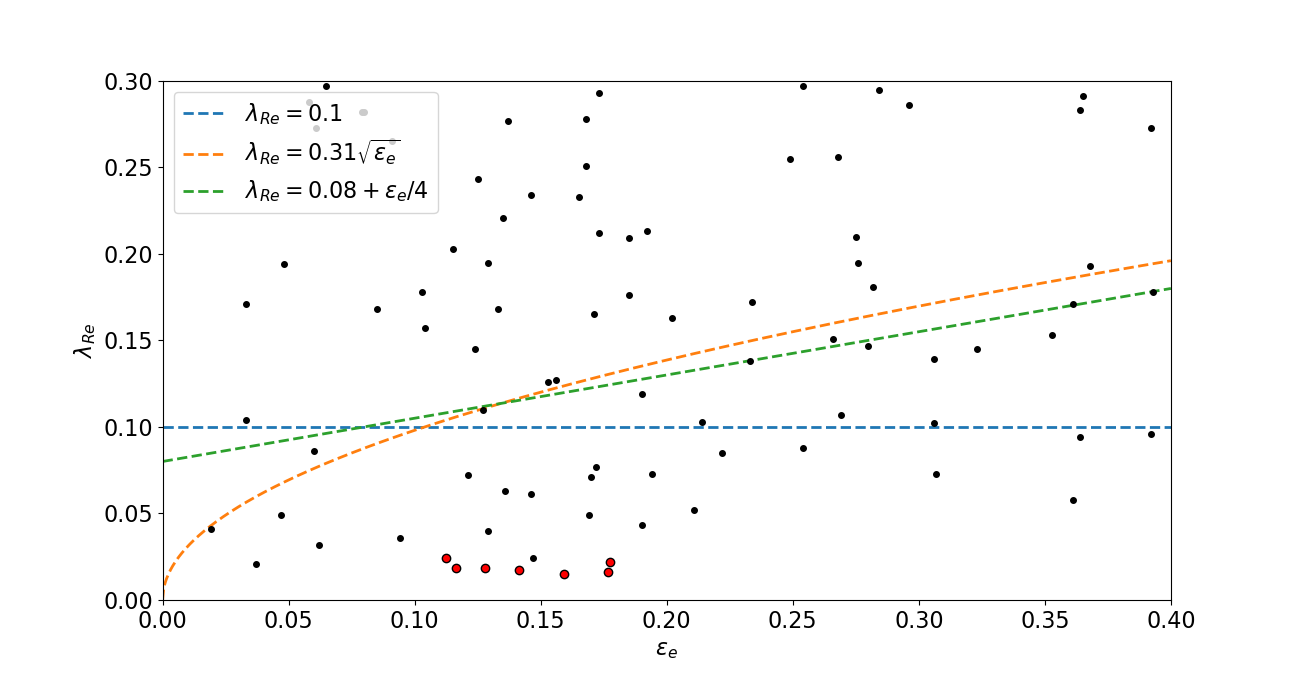
\includegraphics[width=\textwidth]{lambda_epsilon.png}
	\caption{Values of the $\lambda_{\mathrm{Re}}$-parameter of galaxies, plotted against their ellipticity at the effective radius. The red dots correspond to the simulated merger remnants, whereas the black dots correspond to galaxies observed in the $\mathrm{ATLAS^{3D}}$-survey \citep{Cappellari2011, Emsellem2011}. The dashed lines display different slow rotator thresholds as a function of ellipticity \citep{Emsellem2007, Emsellem2011, Cappellari2016}.}
	\label{figure:lambda_epsilon}
\end{figure}

Regardless of the threshold used for differentiating between slow and fast rotators, figure \ref{figure:lambda_epsilon} shows us that, all of the simulated merger remnants are clearly classified as slow rotators. This agrees well with the kinematic anisotropies seen in the IFU maps, which also implied a slow rotator classification for the remnants.

\section{Comparison to Observations}

As the physical properties of the merger progenitors are modelled after NGC 1600, it is interesting to see how the results from the simulations compare with actual observations of the galaxy. While I will be comparing the observations mainly to the BH-6 merger remnant, as the mass of the SMBH binary in the simulated galaxy is equivalent to the observed and modelled mass of the central SMBH in NGC 1600 ($M_\bullet = 1.7 \times 10^{10} M_\odot$) \citep{Thomas2016}; I will also be comparing the observed properties of the cored massive elliptical galaxy NGC 4472 to the simulated BH-1 merger remnant. Both of the latter galaxies have similar central black hole masses (or in the case of the simulated remnant, black hole binary mass), as well as similar total stellar masses. Thus, comparing their other physical properties could provide some interesting insight into the formation of cores.

Figure \ref{figure:profile_comparison} shows core-Sérsic profile fits of the surface brightness profiles from the BH-1 and BH-6 mergers, and compares them to the profile fits from the observed core galaxies NGC 4472 and NGC 1600 respectively. Not only do the shapes of the compared photometric profiles follow each other closely in both cases, the best-fit parameters are also quite closely related (table \ref{table:bestfit_parameter_comparison}). 

\begin{table}
	\begin{center}
		\scriptsize
		\begin{tabular}{| c | c c | c c |}
		\hline
		 & BH-1 merger & NGC 4472 & BH-6 merger & NGC 1600 \\
		\hline
		$r_b \; \mathrm{[kpc]}$ & $0.137$ & $0.151$ & $0.579$ & $0.667$ \\
		$\mu_b \; \mathrm{[mag \, arcsec^{-2}]}$ & $16.29$ & $16.48$ & $17.68$ & $18.00$ \\
		$R_e \; \mathrm{[kpc]}$ & $9.717$ & $16$ & $9.304$ & $16.04$ \\
		$n$ & $4$ & $5.6$ & $4$ & $5.83$ \\
		$\alpha$ & $1.45$ & $3.05$ & $1.22$ & $2.09$ \\
		$\gamma$ & $0.00$ & $0.06$ & $-0.04$ & $0.03$ \\
		\hline
		\end{tabular}
	\end{center}
	\caption{Best-fit parameters of the core-Sérsic profile fits seen in figure \ref{figure:profile_comparison}. The best-fit parameters of NGC 4472 are from \cite{Rusli2013}, while the parameters for NGC 1600 are given in \cite{Thomas2016}. $n$ is the Sérsic index, $\alpha$ controls the sharpness of the transition between the inner and outer profiles, and $\gamma$ is the slope of the inner profile.}
	\label{table:bestfit_parameter_comparison}
\end{table}

Another comparison between some of the properties of the four galaxies can be seen in table \ref{table:snap6_vs_NGC1600}. Most importantly, the table shows that the kinematic properties of the simulated merger remnants and the kinematic properties of NGC 1600 are very similar. On the other hand, compared to the three other galaxies, the spin parameter and line-of-sight velocity of NGC 4472 are almost an order of magnitude larger. Furthermore, like the simulated galaxies, NGC 1600 can easily be identified as a slow rotator by its $\lambda_e$ parameter and ellipticity, while NGC 4472 seems to be classified as a fast rotator. 

Before drawing conclusion from these results, it is important to know that, whether NGC 4472 is in fact classified as a fast rotator is not known for certain. \cite{Emsellem2011} found a significantly lower value for its spin parameter ($\lambda_e = 0.077$), which would easily classify the object as a slow rotator. The value used in this analysis comes from the more recent MASSIVE-survey \citep{Ma2014MASSIVE, Veale2017veldisp}, in which some of the inaccuracies of the previous observations were shown (e.g. not taking into account a large enough region of the observed galaxy). Conceding to some possible biases in their own calculations, \cite{Veale2017veldisp} ultimately classify NGC 4472 as an intermediate case between slow and fast rotators.

It is impressive, that the simulation of the BH-6 merger is able to reproduce both the kinematic properties and the shape of the surface brightness profile of NGC 1600 so well. Since the simulation describes a dry major merger event between two massive ETG with central SMBHs, the results imply that this process could be the formation mechanism behind core galaxies. 

Interestingly, since the BH-6 merger has extremely similar kinematic properties with the BH-1 merger and NGC 1600, it can be assumed that the mass of the central SMBH binary does not affect the rotation of its host galaxy in any significant way. This suggests that, as far as the merger progenitors are concerned, it is the properties other than their central SMBH mass (i.e. them being massive gas-poor ETGs) that determine the stellar kinematics in the final merger remnant. As for NGC 4472, since both its $\lambda_e$ and LOS velocity are about an order of magnitude larger compared to the three other galaxies, it can be argued that its formation history must be quite different when compare to the other galaxies. However, due to the ambiguity of whether NGC 4472 is a fast rotator and whether its spin parameter is biased towards large values, the possibility that the galaxy has also formed through a dry ETG merger, should not be ruled out.

Earlier in this chapter it was shown that there is a clear positive correlation between the central SMBH binary masses and the size of the core radii. However, the fact that the core radius sizes for the BH-1 merger remnant and NGC 4472 are comparable, and that many of their other properties are quite different; imply that, not only is there a correlation, the SMBH binary mass might be the only property that affects the size of the core in any significant way. If this is true, it is very strong evidence, that the cores are formed through a scouring process by binary SMBHs.


\begin{table}
	\begin{center}
		\scriptsize
		\begin{tabular}{c c c c c c c c c c}
		\hline
		\hline
		Galaxy & $M_\star$ & $M_\bullet$ & $R_e$ & $\mu_e$ & $n$ & 
		$V_\mathrm{LOS}$ & $\sigma_e$ & $\lambda_e$ &
		$\epsilon_e$ \\
		& $[\times 10^{11} M_\odot]$ & $[\times 10^{10} M_\odot]$ &
		[kpc] & [$\mathrm{mag/arcsec^2}$] & & [km/s] & [km/s] & & \\
		(1) & (2) & (3) & (4) & (5) & (6) & (7) & (8) & (9) & (10) \\
		\hline
		BH-6 merger & $8.3$ & $1.7$ & $10.722$ & $21.54$ & $4$ & $5.61$ & $278$ & $0.0213$ & $0.15$ \\
		NGC 1600 & $8.3$ & $1.7$ & $\sim 16$ & $\sim 22.8$ & $5.83$ & $7.1$ & $293$ & $0.026$ & $0.32$ \\
		\hdashline
		BH-1 merger & $8.3$ & $0.17$ & $9.879$ & $21.42$ & $4$ & $5.49$ & $274$ & $0.021$ & $0.195$ \\
		NGC 4472 & $6.03$ & $0.25$ & $14.33$ & $22.72$ & $5.6$ & $45.4$ & 
		$258$ & $0.197$ & $0.172$ \\
		\hline
		\end{tabular}
	\end{center}
	\caption{Comparisons between the physical properties of the simulated BH-1 and BH-6 merger remnants and the observed galaxies NGC 1600 and NGC 4472 respectively. The properties described in the columns are explained below, alongside the sources for their values in NGC 1600 and NGC 4472. \\
	(1) Name of the galaxy. \\
	(2) Total stellar mass. NGC 1600: \cite{Thomas2016}, NGC 4472: \cite{Veale2018lambda}. \\
	(3) Central SMBH / central SMBH binary mass. NGC 1600:  \cite{Thomas2016}, NGC 4472: \cite{Rusli2013_BHmass}. \\
	(4) Effective radius. The values used for the simulated mergers are estimated by calculating the half-mass radius in three dimensions, and using equation \ref{eq:projection_approximation} to get the approximate two dimensional effective radius. This is done instead of using the core-Sérsic profile best-fit parameter, since the core-Sérsic $R_e$ only takes into account the specific fitting radius. NGC 1600: \cite{Thomas2016}, where the value is changed from arc seconds to kpc by assuming that the galaxy is located at the distance of $D = 64 \; \mathrm{Mpc}$; NGC 4472: \cite{Veale2017veldisp}. \\
	(5) Surface brightness at the effective radius. The values for all of the galaxies are calculated from the core-Sérsic fits. The profile fits best-fit parameters are from table \ref{table:bestfit_parameter_comparison}. \\
	(6) Sérsic index. NGC 1600: \cite{Thomas2016}, NGC 4472: \cite{Rusli2013}. \\
	(7) Mean line-of-sight velocity inside the effective radius. For the the simulated mergers these values are calculated from their respective IFU maps as the mean of the $V_{LOS}$-values from the Voronoi-bins inside the effective radius. NGC 1600 and NGC 4472: \cite{Bender1994}. \\
	(8) Velocity dispersion inside the effective radius. As with $V_{LOS}$, this value comes from the mean velocity dispersion of the Voronoi bins inside the effective radius in the IFU-maps for the simulated mergers. NGC 1600 and NGC 4472: \cite{Veale2017veldisp}.\\
	(9) Spin parameter at the effective radius. NGC 1600 and NGC 4472: \citep{Veale2018lambda}. \\
	(10) For the simulated mergers and NGC 4472: ellipticity of the galaxy at the effective radius. For NGC 1600: luminosity weighted ellipticity. NGC 1600: \cite{Goullaud2018}, NGC 4472: \cite{Emsellem2011}.
	}
	\label{table:snap6_vs_NGC1600}
\end{table}

\begin{figure}
	\centering
	\begin{subfigure}[b]{0.49\textwidth}
		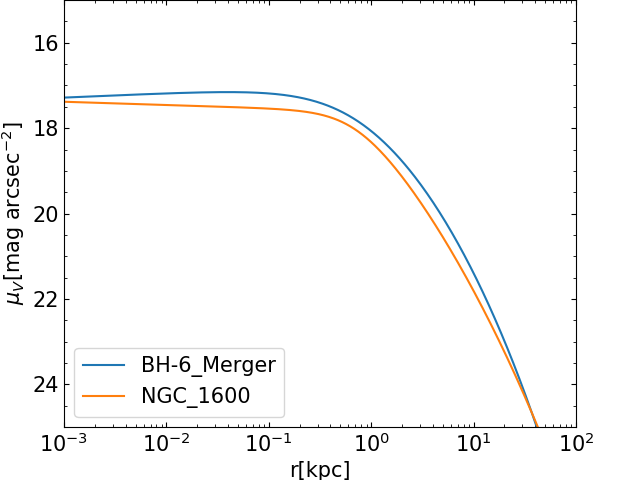
\includegraphics[width=\textwidth]{BH-6_NGC1600.png}
	\end{subfigure}
	\begin{subfigure}[b]{0.49\textwidth}
		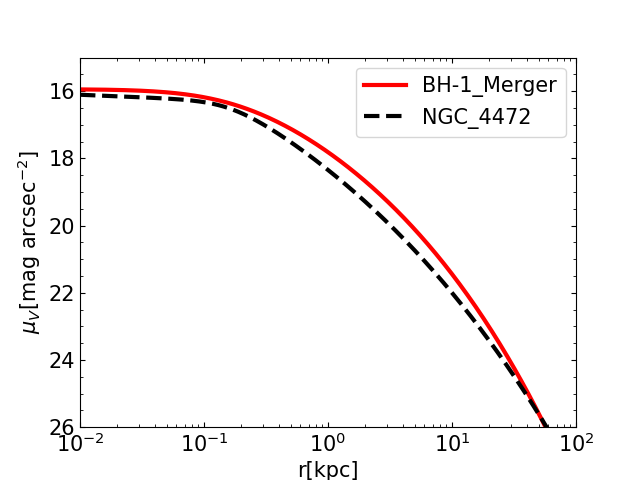
\includegraphics[width=\textwidth]{BH-1_NGC4472.png}
	\end{subfigure}
	\caption{Comparison between core-Sérsic profile fits from observed galaxies and simulated merger remnants, where the surface brightness is given in V-band magnitudes. The figure on the left compares the profile of the BH-6 merger remnant (the merger remnant whose progenitors containing the largest central SMBH masses) to NGC 1600; while the figure on the right compares the profiles of the BH-1 merger remnant (the remnant with progenitors that had the smallest SMBH masses) and NGC 4472. The parameters for plotting the core-Sérsic profile of NGC 1600 were taken from \cite{Thomas2016}, with the units being changed to the above, by assuming $V - R = 0.5$ (the same assumption being done in \cite{Lauer2007}), and by using the distance $D = 64 \mathrm{Mpc}$ \citep{Thomas2016} to define the relation between arc seconds and parsecs. The parameters for the profile of NGC 4472 were from \cite{Rusli2013}. All of the best-fit parameters can be found in table \ref{table:bestfit_parameter_comparison}}
	\label{figure:profile_comparison}
\end{figure}


\chapter{Conclusions}

\appendix

\chapter{Figures}

\begin{figure}
	\centering
	\begin{subfigure}[b]{0.49\textwidth}
		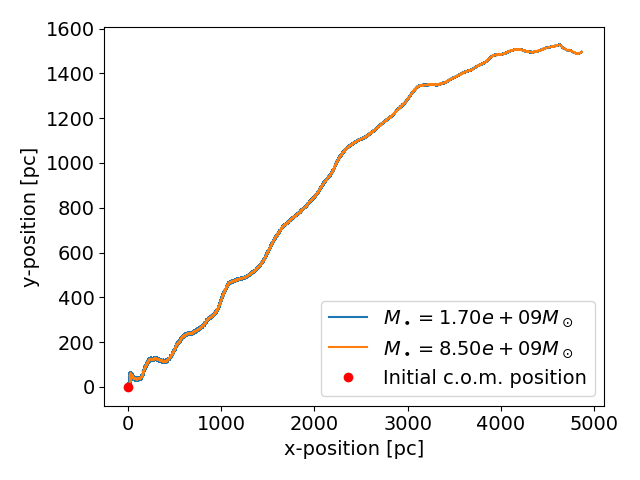
\includegraphics[width=\textwidth]{Run1_Trajectory_small.png}
		\caption{Run 1}
	\end{subfigure}
	\begin{subfigure}[b]{0.49\textwidth}
		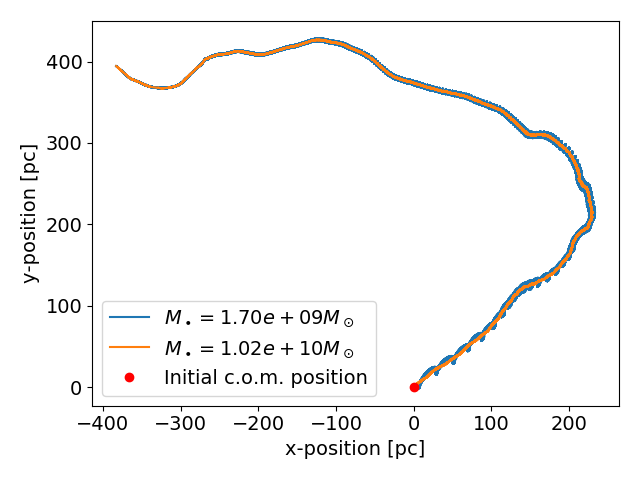
\includegraphics[width=\textwidth]{Run2_Trajectory_small.png}
		\caption{Run 2}
	\end{subfigure}
	\begin{subfigure}[b]{0.49\textwidth}
		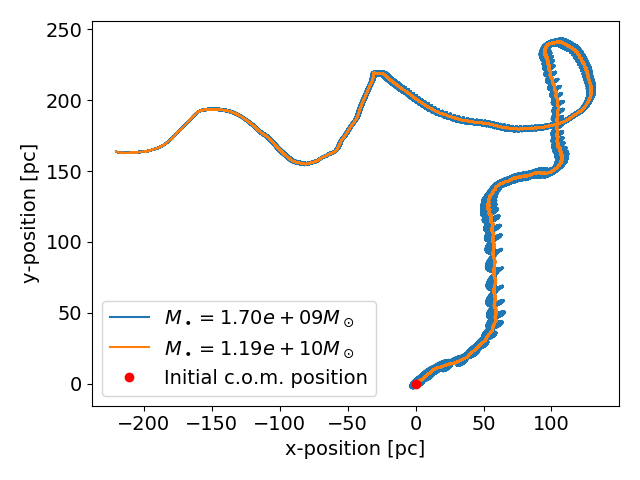
\includegraphics[width=\textwidth]{Run3_Trajectory_small.png}
		\caption{Run 3}
	\end{subfigure}
	\begin{subfigure}[b]{0.49\textwidth}
		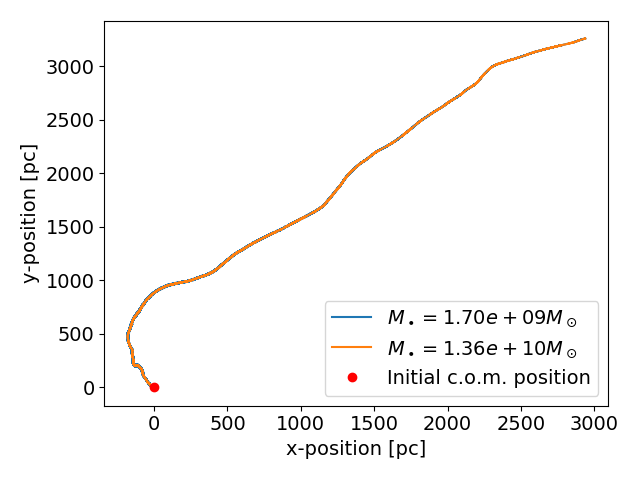
\includegraphics[width=\textwidth]{Run4_Trajectory_small.png}
		\caption{Run 4}
	\end{subfigure}
	\caption{The trajectories of the black holes from simulation runs by \cite{Mannerkoski2019}. The coordinates are centred on the initial location of the centre-of-mass of the black hole system. The orange and blue lines show the paths taken by the smaller and larger black holes respectively during the simulation.}
	\label{figure:all_traj}
\end{figure}

% STEP 5:
% Uncomment the following lines and set your .bib file and desired bibliography style
% to make a bibliography with BibTeX.
% Alternatively you can use the thebibliography environment if you want to add all
% references by hand.


% Define journal names
\newcommand{\apj}{The Astrophysical Journal}
\newcommand{\mnras}{Monthly Notices of the Royal Astronomical Society}
\newcommand{\apjs}{The Astrophysical Journal Supplement}
\newcommand{\nat}{Nature}
\newcommand{\aj}{The Astronomical Journal}
\newcommand{\na}{New Astronomy}
\newcommand{\araa}{Annual Review of Astronomy and Astrophysics}
\newcommand{\aap}{Astronomy and Astrophysics}
\newcommand{\apjl}{The Astrophysical Journal Letters}
\newcommand{\prl}{Physical Review Letters}
\newcommand{\ssr}{Space Science Reviews}
\newcommand{\prd}{Physical Review D}

\clearpage
\addcontentsline{toc}{chapter}{Bibliography} % This lines adds the bibliography to the ToC
\bibliographystyle{plainnat}
\bibliography{bibliography.bib}


\end{document}

